\newcommand*{\pth}{$p^{H}_{\text{T}}$\xspace}
\newcommand*{\htautau}{$H \to \tau \tau$\xspace}
\newcommand*{\ztautau}{$Z \to \tau \tau$\xspace}
\newcommand*{\pt}{$p_{\text{T}}$\xspace}
\newcommand*{\taul}{$\tau$-lepton\xspace}
\newcommand*{\tauhadvis}{\ensuremath{\tauhad}\xspace}
\newcommand*{\mmc}{\ensuremath{m^\text{MMC}_{\tau\tau}}\xspace}
\newcommand*{\taulephad}{$\tau_{\text{lep}}\tau_{\text{had}}$\xspace}
\newcommand*{\tauhadhad}{$\tau_{\text{had}}\tau_{\text{had}}$\xspace}
\newcommand*{\tauemu}{$\tau_{e}\tau_{\mu}$\xspace}
\newcommand*{\mtt}{\ensuremath{m_{\tau\tau}}\xspace}


This chapter presents the core analysis developed in the context of this thesis, focusing on the study of the Higgs boson decay into a pair of $\tau$-leptons produced in association with top-quark pairs. This \ttHtt final state is of particular importance, both because of its experimental challenges and because it provides unique sensitivity to the top-Higgs Yukawa interaction. The following sections describe the motivation behind this measurement, the general and specific strategy pursued in ATLAS, the definition of physics objects and event selection, and the improvements introduced during this work with respect to earlier iterations of the analysis. Special emphasis is given to the implementation of MVA for event categorization.


%%%%%%%%%%%%%%%%%%%%%%%%%%%%%%%%%%%%%%%%%%%%%%%%%%%%%%%%%%%%%%%%%%%%%%%%%%%%%%%%%%%%%%%%%%%%%%%%%%%%%%%%%%%%%%%%%%%%%%%%%%%%%%%%%%%%%%%%%%%%%%%%%%%%%%%%%%%%%%%%%%%%%%%%%%%%%%%%%%%%
\section{Motivation}
\label{sec:analysis_motivation}

The production of the Higgs boson in association with a top-quark pair provides a privileged way to probe the Yukawa coupling between the two particles, $y_{t}$, since the production cross-section of this process is proportional to the square of this coupling, as already discussed in Section~\ref{sec:ttH}. A direct measurement of this parameter is of particular importance both for confirming the properties of the Higgs boson within the SM and for exploring the nature of the EWSB mechanism and potential effects of BSM physics.

As previously mentioned, the $t\bar{t}H$ production mode was first established by ATLAS and CMS in 2018, combining the Higgs boson decays $H \to VV^{*}$, $H \to \tau\tau$, $H \to b\bar{b}$, and $H \to \gamma\gamma$, as illustrated in Figure~\ref{fig:tth_obs}. The results were obtained in terms of the signal strength, $\mu_{t\bar{t}H}$, with an observed excess of $6.3\sigma$ above the SM expectation in ATLAS and $5.2\sigma$ in CMS.

\begin{figure}[htbp]
  \centering
  \begin{subfigure}[b]{0.495\textwidth}
    \centering
    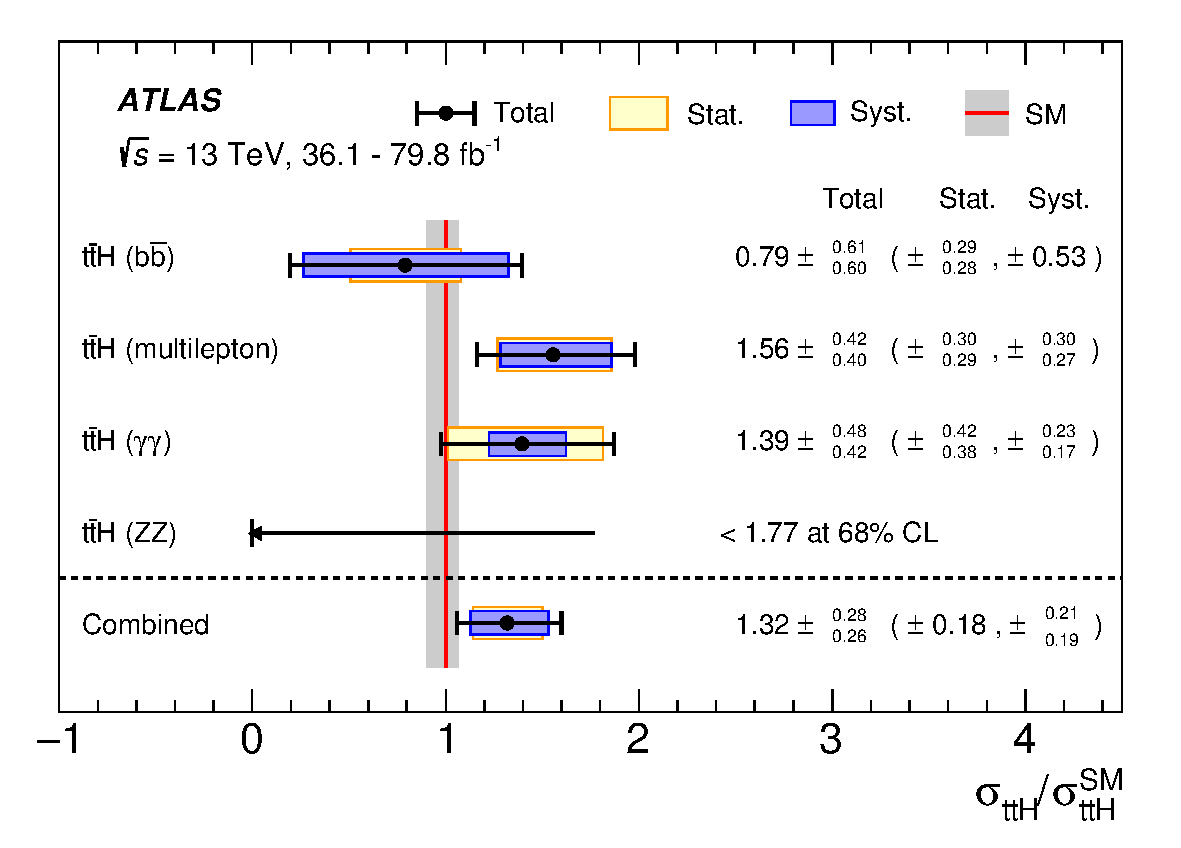
\includegraphics[height=0.55\textwidth]{desv_atlas}
    \caption{}
    \label{fig:tth_obs_atlas}
  \end{subfigure}%
  \hfill
  \begin{subfigure}[b]{0.495\textwidth}
    \centering
    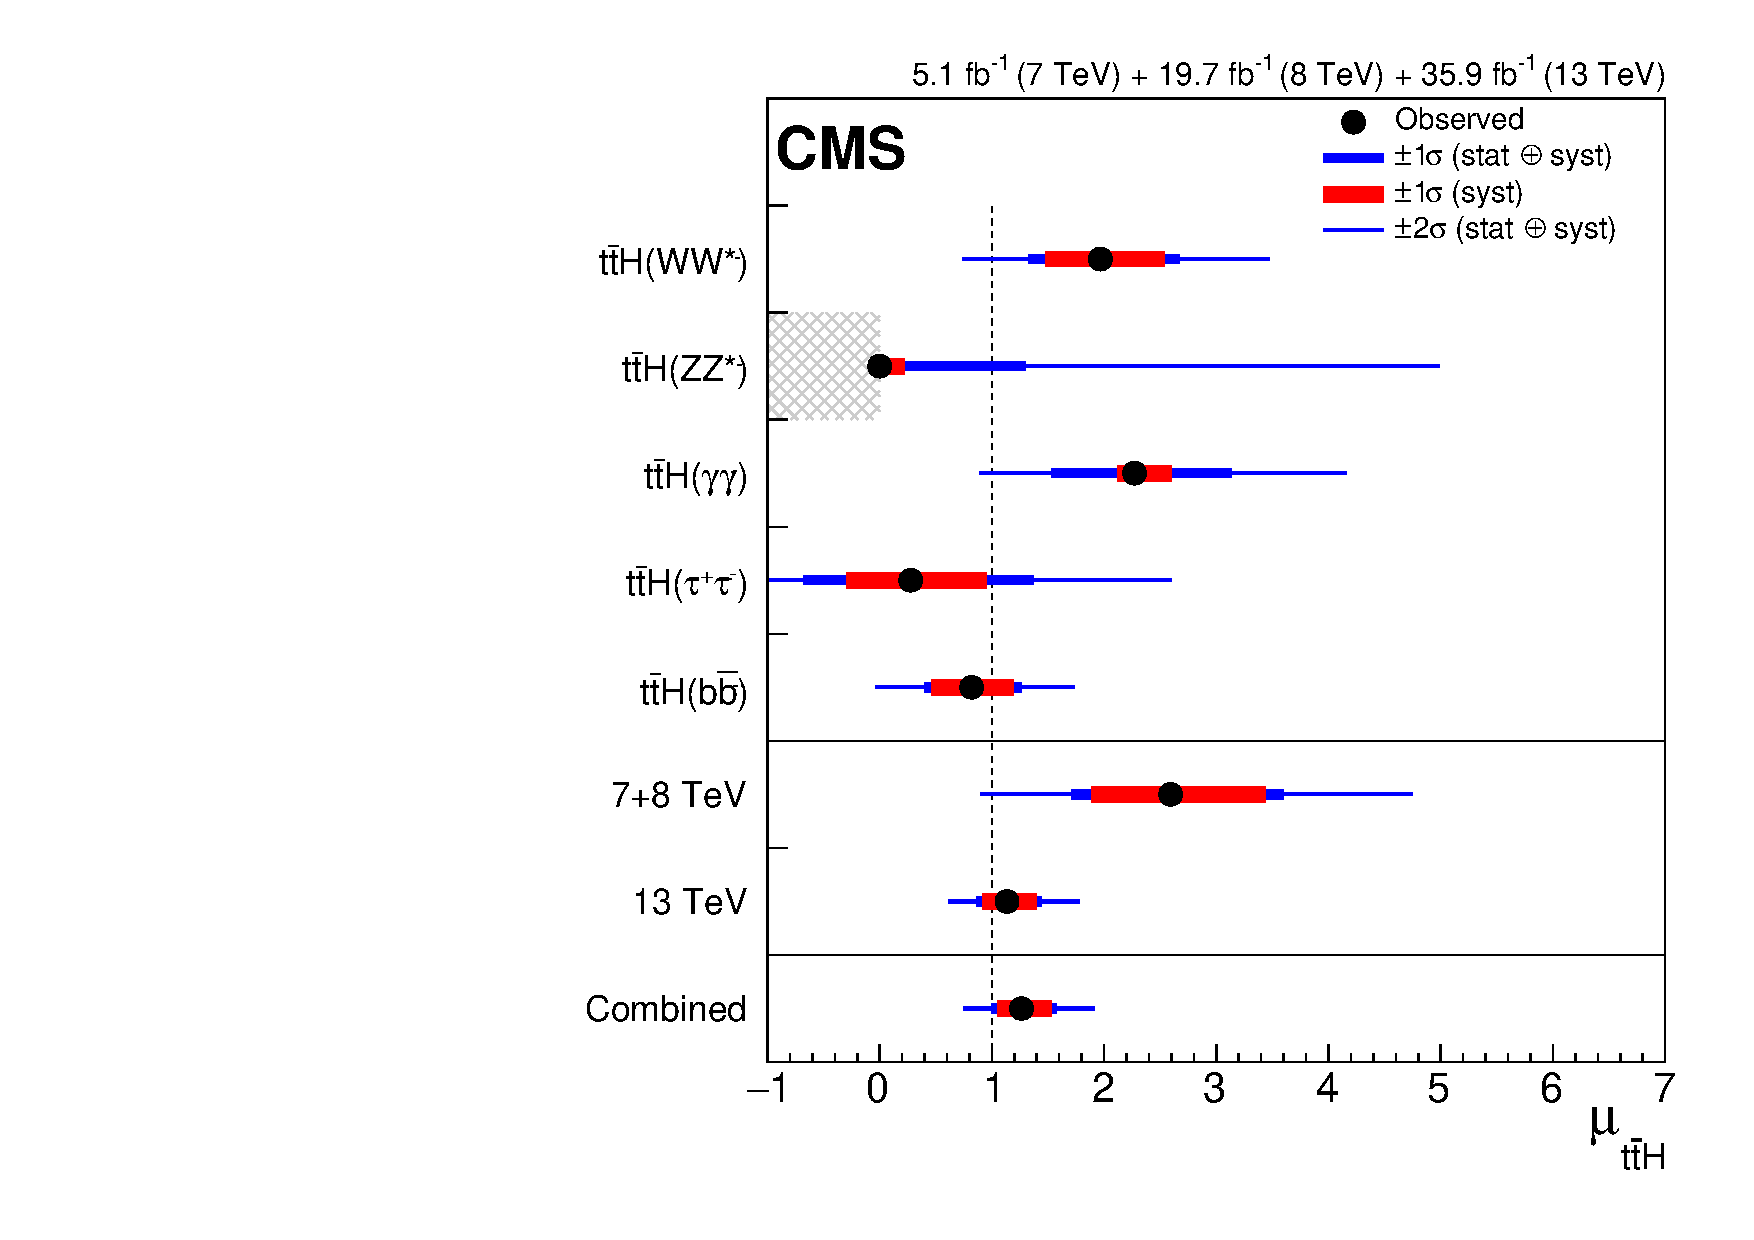
\includegraphics[height=0.55\textwidth]{desv_cms}
    \caption{}
    \label{fig:tth_obs_cms}
  \end{subfigure}
  
  \caption{(a) Combined $t\bar{t}H$ production cross-section together with the individual ATLAS measurements, shown as ratios to the SM prediction~\cite{ATLAS:2018mme}. Black lines represent the total uncertainties, while the bands indicate the statistical and systematic components. (b) Best-fit value of the signal strength $\mu_{t\bar{t}H}$ measured by CMS, including the one- and two-standard-deviation confidence intervals~\cite{CMS:2018uxb}.}
  \label{fig:tth_obs}
\end{figure}


  The \ttH production mode contributes only about 1\% to the total effective Higgs boson production cross-section at the LHC, as indicated in Section~\ref{sec:higgs_production}, with a predicted value of $0.507^{+5.8}_{-9.2} \text{ (QCD scale)} \pm 3.6 \text{ (PDF}+\alpha_{s})$~pb at $\sqrt{s}=13$~TeV~\cite{https://doi.org/10.23731/cyrm-2017-002}. For this reason, the design of a \ttH analysis requires a careful balance between selecting a decay channel with a sufficiently large branching ratio and ensuring good control over the different background contributions.  

  Following the observation of this production mode, subsequent analyses using the Run-2 dataset focused on improving the precision of the measured cross-section by targeting specific regions of phase space and exploiting decay modes that either maximize sensitivity to the signal or provide enhanced sensitivity to possible BSM effects, either individually or in combination with other Higgs production modes. Among the possible decay channels, $H \to b\bar{b}$ appears particularly attractive due to its large Higgs boson branching ratio. However, \ttH analyses in this channel are strongly affected by the overwhelming background from $t\bar{t}b\bar{b}$ production, which is both large and difficult to model~\cite{Aad:2904447}.  
  
  In this thesis, the \htautau decay channel is considered as it offers a balanced compromise between signal yield and background control together with fully hadronic decays of the \ttbar system. Moreover, the reconstruction of the di-$\tau$ system in \htautau events provides additional discrimination power against the dominant backgrounds. As already mentioned, the \ttH analysis with \htautau decays is not grouped together with other multilepton final states, but instead constitutes a dedicated category within the broader \htautau analysis, restricted to the case where both $\tau$-leptons decay hadronically. The remaining $\tau$-decay channels and/or \ttbar decays involving leptons are covered by other ATLAS studies~\cite{PhysRevD.97.072003}.  
  
  The first evidence for the \htautau decay channel was established during Run~1. ATLAS reported a significance of $4.5\sigma$~\cite{htau_2015}, and the combination of ATLAS and CMS confirmed the channel with a significance of $5.5\sigma$~\cite{htau_cms_atlas_2016}. Subsequently, Run-2 analyses concentrated on more precise measurements of the total cross-section as well as on the individual contributions of the main production modes. Differential measurements based on kinematic observables such as the transverse momentum of the Higgs boson (\pth) or the jet multiplicity were also performed, as described in Section~\ref{sec:stxs_yukawa}.  
  
  Among the four main Higgs boson production modes, \htautau has provided the most precise results for the VBF production. The measurement obtained in the first study using the full Run-2 dataset yielded a cross-section of $0.90^{+0.20}_{-0.17}$ times the SM prediction~\cite{2022}, in good agreement with the CMS result of $0.81 \pm 0.17$ times the SM expectation~\cite{Tumasyan_2023}. For \ttH production, the precision was more limited, but still provided sensitivity, with an inclusive measured production cross-section of $1.06^{+1.28}_{-1.08}$ times the SM prediction. These results were originally derived within the STXS framework, with granularity adapted in \pth, the dijet invariant mass ($m_{jj}$), and jet multiplicity, resulting in a total of nine fiducial STXS bins: six targeting ggF production and three devoted to VBF, $VH$, and \ttH, respectively, as shown in Figure~\ref{fig:atlas_htautau_stxs}.
  
\begin{figure}[htbp]
    \centering
    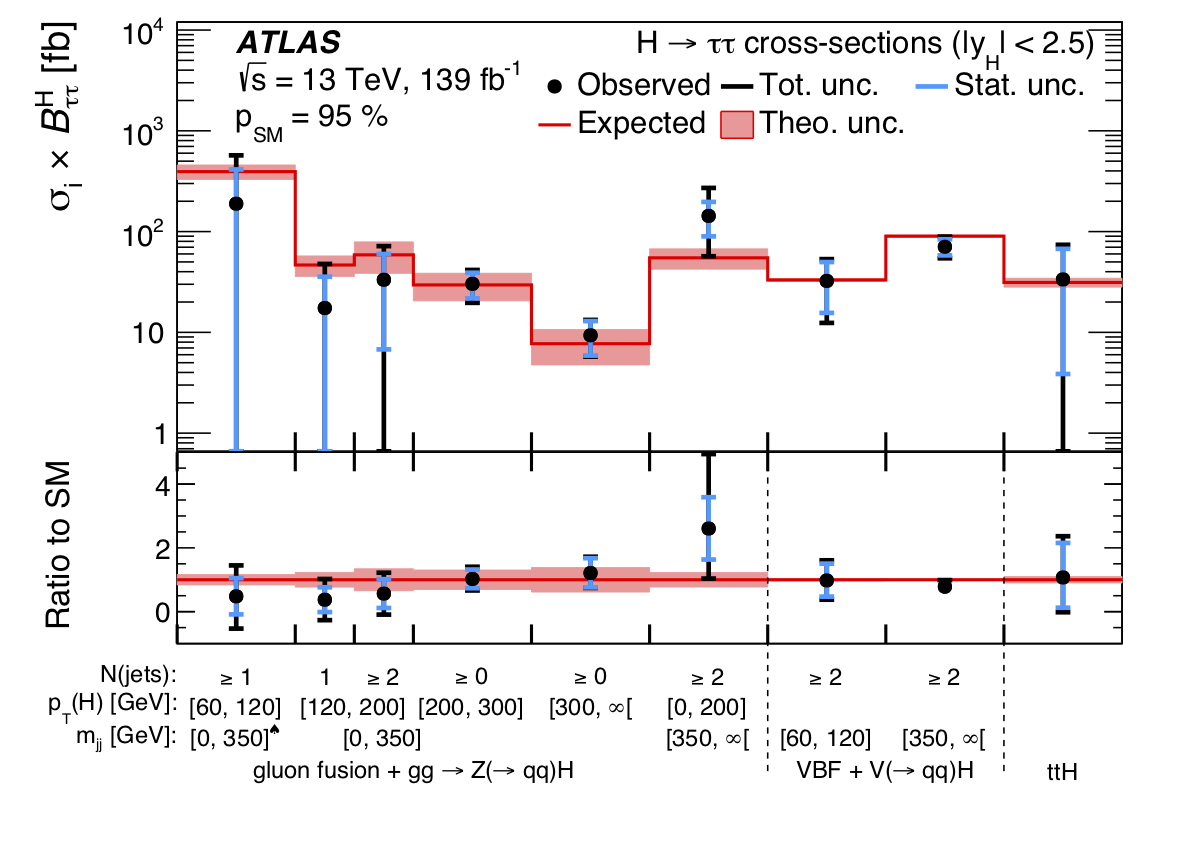
\includegraphics[width=0.7\textwidth]{images/pois_9pois.png}
    \caption{Measured values of $\sigma \times \mathcal{B}(H \to \tau\tau)$ in the nine fiducial regions defined by the STXS framework, from the first ATLAS analysis of $H \to \tau\tau$ using the full Run-2 dataset. Black (blue) error bars represent the total (statistical) uncertainties, while the continuous lines correspond to the SM predictions~\cite{2022}.}
    \label{fig:atlas_htautau_stxs}
\end{figure}

This chapter presents the measurements obtained in the most recent published iteration of the \htautau analysis using the full Run-2 dataset. This new round extends the scope of the STXS results from the previous analysis, including additional STXS bins for both VBF and \ttH.  

In particular, this thesis focuses on the extension of the \ttH analysis within this framework, moving from an inclusive measurement in the fully hadronic final state to the determination of the cross-section in three separate STXS bins in \pth. This strategy potentially increases the sensitivity to deviations from the SM in the high-\pt\ regions.  

Moreover, a more precise measurement of the $t\bar{t}H(H\to\tau\tau)$ channel is of particular importance in the context of the combined Higgs boson measurements performed at ATLAS, where all accessible production and decay modes are simultaneously fitted. In these combinations, significant (anti)correlations have been observed between $t\bar{t}H(H\to\tau\tau)$ and other channels, most notably $t\bar{t}H(H\to WW^*)$, with values reaching up to $-0.45$ in Run-2 fits~\cite{Aad_2020_combined}. Such correlations reduce the overall sensitivity of the combined analyses and limit the ability to disentangle the different Higgs boson production and decay modes. The most recent ATLAS results~\cite{ATLAS-CONF-2025-006} confirm this effect, with updated correlation coefficients of about $-0.30$ between the $H\to\tau\tau$ and $H\to WW^*$ channels in the global signal strength fits.

%%%%%%%%%%%%%%%%%%%%%%%%%%%%%%%%%%%%%%%%%%%%%%%%%%%%%%%%%%%%%%%%%%%%%%%%%%%%%%%%%%%%%%%%%%%%%%%%%%%%%%%%%%%%%%%%%%%%%%%%%%%%%%%%%%%%%%%%%%%%%%%%%%%%%%%%%%%%%%%%%%%%%%%%%%%%%%%%%%%%

\section{Analysis strategy}
\label{sec:analysis_strategy}

The new measurements presented in this thesis are obtained from the analysis of the full Run-2 dataset, corresponding to an integrated luminosity of $140~\text{fb}^{-1}$ at a centre-of-mass energy of $\sqrt{s}=13$~TeV, using the \textsc{athena} rel.21. Although it is a promising channel, \htautau also presents a number of challenges. The final state can be obscured by irreducible background processes, most notably \ztautau, which has a cross-section much larger than that of the Higgs boson, and whose mass peak lies not far from the Higgs boson resonance.  

In addition, while the presence of $\tau$-leptons allows for a good reconstruction of the Higgs boson, it must be taken into account that $\tau$-leptons decay before reaching the detector. The resulting final states are therefore complex, containing neutrinos that escape detection. This complicates the reconstruction of the Higgs boson mass and \pt compared with other cleaner channels such as $H \to \gamma\gamma$.  

Another difficulty arises from the fact that certain reconstructed objects can be misidentified as $\tau$-leptons, which must be carefully controlled. The following sections describe the strategy developed to address these issues in this analysis, focusing on the \ttH production mode. 

Within the global \htautau analysis, events are first categorised according to the decay modes of the $\tau$-leptons into three channels: $\tau_{e}\tau_{\mu}$, $\tau_{\text{lep}}\tau_{\text{had}}$, and $\tau_{\text{had}}\tau_{\text{had}}$. Channels with two electrons or two muons are excluded from the analysis due to their much smaller branching ratios and sensitivity, as they are heavily contaminated by $Z \to \ell\ell$ decays.  

As already mentioned, in \ttHtt only the $\tau_{\text{had}}\tau_{\text{had}}$ final state is considered. In this channel, the dominant background is \ztautau, followed by processes where hadronic $\tau$-lepton decays (\tauhad) are misidentified (referred to as ``Fakes'' or fake background), in which jets are reconstructed as $\tau_{\text{had}}$ candidates.  These fake background events are derived with data-driven techniques to reduce the dependence on simulations.

The $Z+$jets background is estimated with MC simulations and normalised to collision data. The \ttH channel also suffers from large backgrounds originating from \ttbar events, which are considered in cases with zero, one, or two $\tau_{\text{had}}$, the latter being the dominant contribution. These \ttbar background events are also extracted from MC simulations and normalised in dedicated data control regions (CRs). 
Other minor background contributions, such as diboson production and $t\bar{t}+W/Z$, are found to be negligible.  
These are therefore taken directly from simulation, with normalization uncertainties applied.  
Given their very small impact across all the regions considered, the fit cannot meaningfully constrain their normalization, so a conservative treatment is adopted. 

The cross-section measurements are performed within the STXS framework, requiring the definition of signal regions (SRs) targeting the different bins of Stage~1.2 of the STXS strategy (Section~\ref{sec:results_ttH}). In this new round of the \htautau analysis, the six ggF and the $VH$ bins measured in the previous iteration are maintained. The $t\bar{t}H$ production mode is now probed in three $p_{\text{T}}^H$ bins, while VBF production is studied in eight kinematic regions defined by $p_{\text{T}}^H$ and $m_{jj}$. Multivariate analysis techniques are employed in the $VH$, $t\bar{t}H$, and VBF signal regions to enhance the sensitivity to the $H \to \tau\tau$ signal. In addition, inclusive measurements of the total cross-section times branching ratio for $H \to \tau\tau$, as well as of the production-mode cross-sections, are performed.  

The following sections will therefore focus on the new strategy for event categorisation in the \ttH channel using MVA techniques, culminating with the presentation of the \ttHtt results. A general overview of the remaining measurements, including the other production modes in the \htautau analysis, will also be presented, summarising the legacy results of the ATLAS collaboration for this decay channel using the full Run-2 dataset. All these results are published in Ref.~\cite{differential_htautau}.

%%%%%%%%%%%%%%%%%%%%%%%%%%%%%%%%%%%%%%%%%%%%%%%%%%%%%%%%%%%%%%%%%%%%%%%%%%%%%%%%%%%%%%%%%%%%%%%%%%%%%%%%%%%%%%%%%%%%%%%%%%%%%%%%%%%%%%%%%%%%%%%%%%%%%%%%%%%%%%%%%%%%%%%%%%%%%%%%%%%%
\section{Event selection}
\label{sec:object_definiton}

As a standard procedure, the selection of candidate events in this analysis relies on the reconstruction and identification of the main physics objects in the detector: electrons, muons, hadronically decaying $\tau$-leptons, jets, and missing transverse momentum. Based on the number and type of these objects, events can be classified into different final states. The analysis presented here focuses exclusively on the channel with two \tauhad, producing narrow hadronic jets together with neutrinos.  

In the following discussion, electrons and muons appearing in the final state will be collectively referred to as light leptons ($\ell$).

\subsection{Trigger criteria}
\label{subsec:trigger_tth}

The first step in defining the events of interest for the analysis is the trigger selections to be applied. The corresponding trigger efficiencies in MC are corrected to match those observed in data using scale factors.  

For the $\tau_{\text{had}}\tau_{\text{had}}$ channel, di-$\tau$ triggers are employed. The two $\tau_{\text{had-vis}}$ candidates reconstructed offline are required to match the corresponding legs of the online di-$\tau$ trigger objects, within $\Delta R < 0.6$. The offline \pt requirements are chosen to ensure that the selected $\tau_{\text{had}}$ candidates lie within the trigger efficiency plateau. Specifically, the leading $\tau_{\text{had}}$ candidate must satisfy an online (offline) requirement of $p_{\text{T}} > 35~(40)$~GeV, while the subleading one must exceed $p_{\text{T}} > 25~(30)$~GeV.  

Due to the increased instantaneous luminosity during the 2016--2018 data-taking period, an additional Level-1 calorimeter jet trigger with online $p_{\text{T}} > 25$~GeV and $|\eta| < 3.2$ was introduced. To guarantee that the trigger operates consistently within its efficiency plateau, the leading jet in the event is required to have $p_{\text{T}} > 70$~GeV and $|\eta| < 3.2$. The impact of this condition on the signal efficiency has been verified to be below $0.3\%$.

\subsection{Physics objects definition}
\label{subsec:object_def}

The procedure followed for the reconstruction and identification of the physics objects used in this analysis closely follows what has already been described in Chapter~\ref{chap:object_rec}.  
In the \ttHtt analysis, only jets with \pt$>20$~GeV are considered. The JVT requirement is applied to jets with \pt$ < 60$~GeV and $|\eta| < 2.5$ in order to suppress those not associated with the primary vertex, while for jets with \pt$ < 60$~GeV in the forward region ($|\eta| > 2.5$) the fJVT is applied. In the \ttHtt process, the most relevant jets, such as $b$-jets from the top-quark decays and the $\tau_{\text{had}}$ candidates, are predominantly located in the central region of the detector. This is in contrast to processes such as VBF, where the characteristic signature involves forward jets. Figure~\ref{fig:tth_topo} shows two examples of tree-level Feynman diagrams for the \ttHtt process.
\begin{figure}[htbp]
    \centering
    \begin{subfigure}[b]{0.48\textwidth}
        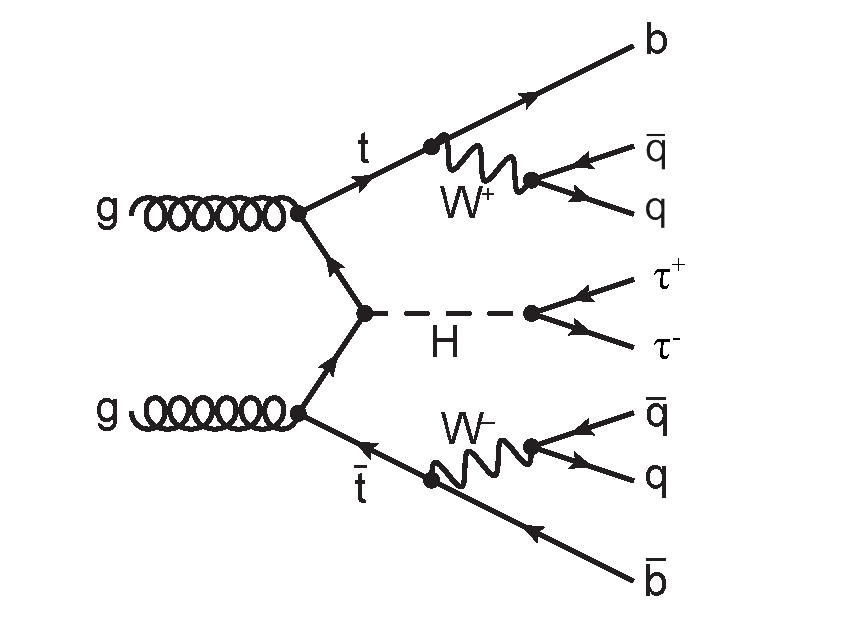
\includegraphics[width=\textwidth]{tth_diagram_1}
    \end{subfigure}
    \hfill
    \begin{subfigure}[b]{0.48\textwidth}
        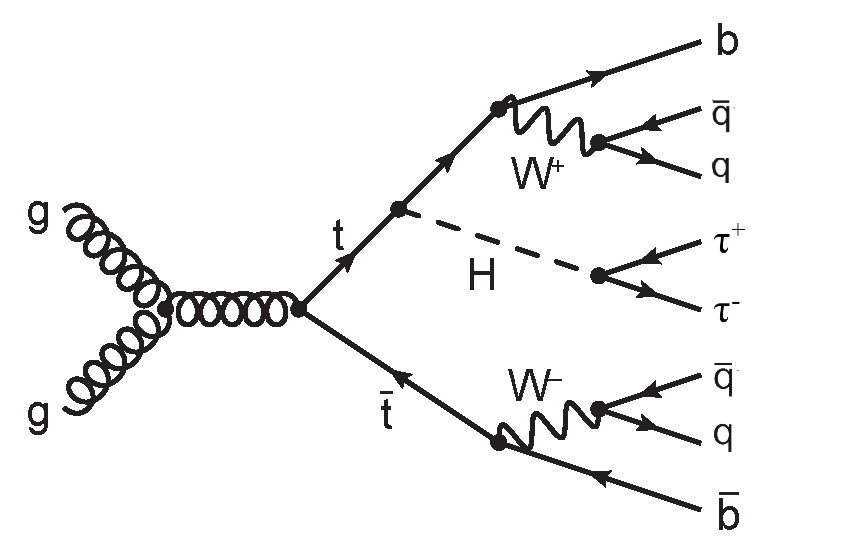
\includegraphics[width=\textwidth]{tth_diagram_2}
    \end{subfigure}
    \hfill
    \caption{Example of tree level diagrams for the \ttHtt process considered in this analyisis.}
    \label{fig:tth_topo}
\end{figure}
\FloatBarrier
The $b$-tagged jets are identified using the DL1r algorithm, with a working point corresponding to a fixed efficiency of $70\%$.  

Referring to $\tau_{\text{had-vis}}$ as the detectable products of \tauhad decays, the selected $\tau_{\text{had-vis}}$ candidates are required to have \pt$ > 20$~GeV and $|\eta| < 2.47$, excluding the transition region between the barrel and end-cap calorimeters. The charge of the $\tau_{\text{had-vis}}$ candidates is computed as the sum of the charges of the associated tracks, and is required to be $\pm 1$. Candidates are further classified as 1-prong or 3-prong, depending on the number of associated tracks. As discussed in Section~\ref{sec:tauhad}, an RNN is employed to discriminate $\tau_{\text{had-vis}}$ from quark- or gluon-initiated jets, while the dedicated eBDT is used to suppress electrons misidentified as $\tau_{\text{had-vis}}$. For this analysis, the Medium identification working point is adopted, providing efficiencies of about $75\%$ and $60\%$ for 1-prong and 3-prong $\tau_{\text{had-vis}}$, respectively.  

Finally, the missing transverse momentum, \etmiss, in the events considered for this study is reconstructed as defined in Section~\ref{sec:met}.

%%%%%%%%%%%%%%%%%%%%%%%%%%%%%%%%%%%%%%%%%%%%%%%%%%%%%%%%%%%%%%%%%%%%%%%%%%%%%%%%%%%%%%%%%%%%%%%%%%%%%%%%%%%%%%%%%%%%%%%%%%%%%%%%%%%%%%%%%%%%%%%%%%%%%%%%%%%%%%%%%%%%%%%%%%%%%%%%%%%%
\section{Higgs boson reconstruction}
\label{sec:higgs_reconstruction}

A crucial ingredient of the \htautau analysis, and in particular for \ttHtt, is the reconstruction of the Higgs boson system from the two $\tau$-leptons. In particular, the di-$\tau$ invariant mass constitutes the primary discriminating variable between the Higgs boson signal and the dominant irreducible background $Z\to\tau\tau$, as well as from reducible contributions such as $t\bar{t}$ events with misidentified $\tau_{\text{had}}$ candidates. 

As mentioned above, the Higgs boson \pt is used to define the \ttH STXS bins that will be used.

\subsection{Higgs boson mass reconstruction}
\label{subsec:higgs_pt}

Since each $\tau$-lepton decay involves one or more neutrinos that escape detection, the full invariant mass cannot be reconstructed directly, and dedicated algorithms are required. In this analysis two approaches are employed: the collinear approximation and the Missing Mass Calculator (MMC).  

The collinear approximation assumes that the neutrinos are emitted in the same direction as the visible $\tau$-lepton decay products. Under this hypothesis, the missing transverse momentum is entirely attributed to the neutrinos, and the momentum fractions $x_1$ and $x_2$ carried by each \taul's visible decay products can be expressed as: 
\begin{align}
    x_{1} &= 
    \frac{p_{x,2}^{\text{vis}} p_{y,1}^{\text{vis}} - p_{y,2}^{\text{vis}} p_{x,1}^{\text{vis}}}
         {p_{x,2}^{\text{vis}} p_{y,1}^{\text{vis}} - p_{y,2}^{\text{vis}} p_{x,1}^{\text{vis}} 
          + E_{x}^{\text{miss}} p_{y,1}^{\text{vis}} - E_{y}^{\text{miss}} p_{x,1}^{\text{vis}}}, \nonumber \\[8pt]
    x_{2} &= 
    \frac{p_{x,2}^{\text{vis}} p_{y,1}^{\text{vis}} - p_{y,2}^{\text{vis}} p_{x,1}^{\text{vis}}}
         {p_{x,2}^{\text{vis}} p_{y,1}^{\text{vis}} - p_{y,2}^{\text{vis}} p_{x,1}^{\text{vis}} 
          - E_{x}^{\text{miss}} p_{y,2}^{\text{vis}} + E_{y}^{\text{miss}} p_{x,2}^{\text{vis}}}.
    \end{align}
being the $x$ and $y$ subscripts the cartesian components of the missing tranverse momentum in the transverse plane. Once the momentum fractions are determined from there, the reconstructed collinear di-$\tau$ mass is
\begin{equation}
m_{\tau\tau}^{\text{coll}} = \frac{m_{\text{vis}}}{\sqrt{x_{1}x_{2}}},
\label{eq:mcoll}
\end{equation}
where $m_{\text{vis}}$ is the visible invariant mass of the two $\tau_{\text{had-vis}}$ candidates, obtained considering only the visible decay products of the \taul. This method provides reasonable resolution in boosted topologies, but can yield unphysical solutions or large overestimates when the collinearity assumption is not valid.  

The Missing Mass Calculator (MMC)~\cite{Elagin_2011} is a more advanced approach designed to overcome the limitations of the collinear approximation. It aims to reconstruct the most probable kinematic configuration of the full di-$\tau$ system, including the invisible neutrinos, by maximizing a likelihood function built from probability density functions derived from $\tau$-decay kinematics. In this framework, six to eight unknown parameters are required to fully describe the event, depending on the $\tau$-lepton decay mode. These variables include the components of the invisible neutrino momenta $\vec{p}^{\,\text{miss}}_{1(2)}$ from each $\tau$ decay, as well as the invariant mass of the invisible system $m^{\text{miss}}_{1(2)}$ for each leptonically decaying $\tau$-lepton. The estimation of these quantities relies on the following mass-shell constraints:
\begin{align}
E_x^{\text{miss}} &= p_1^{\text{miss}} \sin \theta^{\text{miss}}_1 \cos \phi^{\text{miss}}_1 + p_2^{\text{miss}} \sin \theta^{\text{miss}}_2 \cos \phi^{\text{miss}}_2 , \nonumber \\
E_y^{\text{miss}} &= p_1^{\text{miss}} \sin \theta^{\text{miss}}_1 \sin \phi^{\text{miss}}_1 + p_2^{\text{miss}} \sin \theta^{\text{miss}}_2 \sin \phi^{\text{miss}}_2 , \nonumber \\
m_{\tau_1}^2 &= \left(m_1^{\text{miss}}\right)^2 + \left(m_1^{\text{vis}}\right)^2 + 2 E_1^{\text{vis}} E_1^{\text{miss}}
- 2 p_1^{\text{vis}} p_1^{\text{miss}} \cos\left(\theta_1^{\text{vis}} - \theta_1^{\text{miss}}\right) ,  \nonumber \\
m_{\tau_2}^2 &= \left(m_2^{\text{miss}}\right)^2 + \left(m_2^{\text{vis}}\right)^2 + 2 E_2^{\text{vis}} E_2^{\text{miss}}
- 2 p_2^{\text{vis}} p_2^{\text{miss}} \cos\left(\theta_2^{\text{vis}} - \theta_2^{\text{miss}}\right) .
\end{align}

Here, $E^{\text{vis}}_{1(2)}$ and $p^{\text{vis}}_{1(2)}$ denote the energies and momenta of the visible $\tau$-decay products, $m^{\text{vis}}_{1(2)}$ their invariant masses, and $m^{\text{miss}}_{1(2)}$ the invariant mass of the neutrino system. The polar (azimuthal) angles of the visible and invisible decay products are given by $\theta^{\text{vis}}_{1(2)}$ ($\phi^{\text{vis}}_{1(2)}$) and $\theta^{\text{miss}}_{1(2)}$ ($\phi^{\text{miss}}_{1(2)}$), respectively. For \tauhad, only one neutrino is produced, so $m^{\text{miss}}_{1(2)}$ is set to zero.  

Even with the above mass-shell constraints, the system remains underdetermined. The MMC addresses this by employing probability density functions derived from $\tau$-lepton decay kinematics, estimated from MC simulations. The algorithm scans over the unknown neutrino parameters and selects the most probable configuration by maximizing a likelihood. To mitigate the impact of the resolution of the missing transverse momentum \etmiss, additional scans over $E_x^{\text{miss}}$ and $E_y^{\text{miss}}$ are performed, with each point weighted according to a Gaussian probability based on the calorimeter’s transverse energy sum.  

The MMC provides different estimators of the di-$\tau$ mass, namely the maximum weight (MAXW), the most likely mass (MLM), and the most likely neutrino momenta (MLNU3P), all obtained through Markov Chain Monte Carlo sampling. Among these, the MLM~\cite{mlm_thesis} method is adopted as the nominal choice, as it defines the reconstructed di-$\tau$ mass from the maximum of the likelihood-weighted histogram of sampled points, yielding the most stable estimate across a wide range of topologies.  

The MMC fails to converge in a small fraction of events (about $1\%$ for the $\tau_{\text{had}}\tau_{\text{had}}$ channel). To avoid losing these events, the $m_{\tau\tau}^{\text{coll}}$ mass from Eq.~(\ref{eq:mcoll}) is used as a fallback. In this way, the MMC–MLM combined with the collinear approximation (\mmc) serves as the primary invariant mass estimator throughout the analysis, ensuring both accuracy and completeness of the event sample. 

\subsection{Reconstruction of \pth}
\label{subsec:higgs_mass}

In the $H \to \tau\tau$ analysis, the transverse momentum of the Higgs boson, $p_{\text{T}}^H$, plays a central role in the categorization of events within the STXS framework. Traditionally, this observable was reconstructed the four-momenta of the visible $\tau$-leptons together with the \etmiss.

In this analysis, a novel neural network (NN) regression is employed to enhance the reconstruction of $p_{\text{T}}^H$. The NN is trained on simulated Higgs events and uses four input variables: the angular separation $\Delta R_{\tau\tau}$, the azimuthal angle difference $\Delta \phi_{\tau\tau}$ between the two $\tau$-leptons, the transverse momentum of the system formed by their four-momenta and \etmiss, and the collinear mass $m_{\tau\tau}^{\text{coll}}$. Although the network is trained using ggF production events, it can be directly applied to the \ttHtt channel or other production modes like VBF without requiring retraining, while still yielding a significant improvement in resolution compared to the traditional method.
This enhancement can be directly observed in Figure~\ref{fig:ptH_resolution}, where the resolution of both reconstruction methods is compared in VBF-produced Higgs boson events. The distribution is significantly narrower, yielding an improvement of approximately $50\%$.

The improved reconstruction of $p_{\text{T}}^H$ reduces bin-to-bin migrations in the STXS framework, thereby providing a more faithful mapping between reconstructed and truth-level distributions. This improvement is particularly exploited in the design of the MVA strategy used to discriminate $t\bar{t}H$ signal events from background, by splitting the training into two $p_{\text{T}}^H$ regions, which increases the sensitivity of the STXS measurement. The NN-based reconstruction therefore not only improves the intrinsic resolution of the observable but also strengthens the overall categorization strategy by enabling a more precise separation of events across the $p_{\text{T}}^H$ spectrum.

\begin{figure}[htbp]
    \centering
    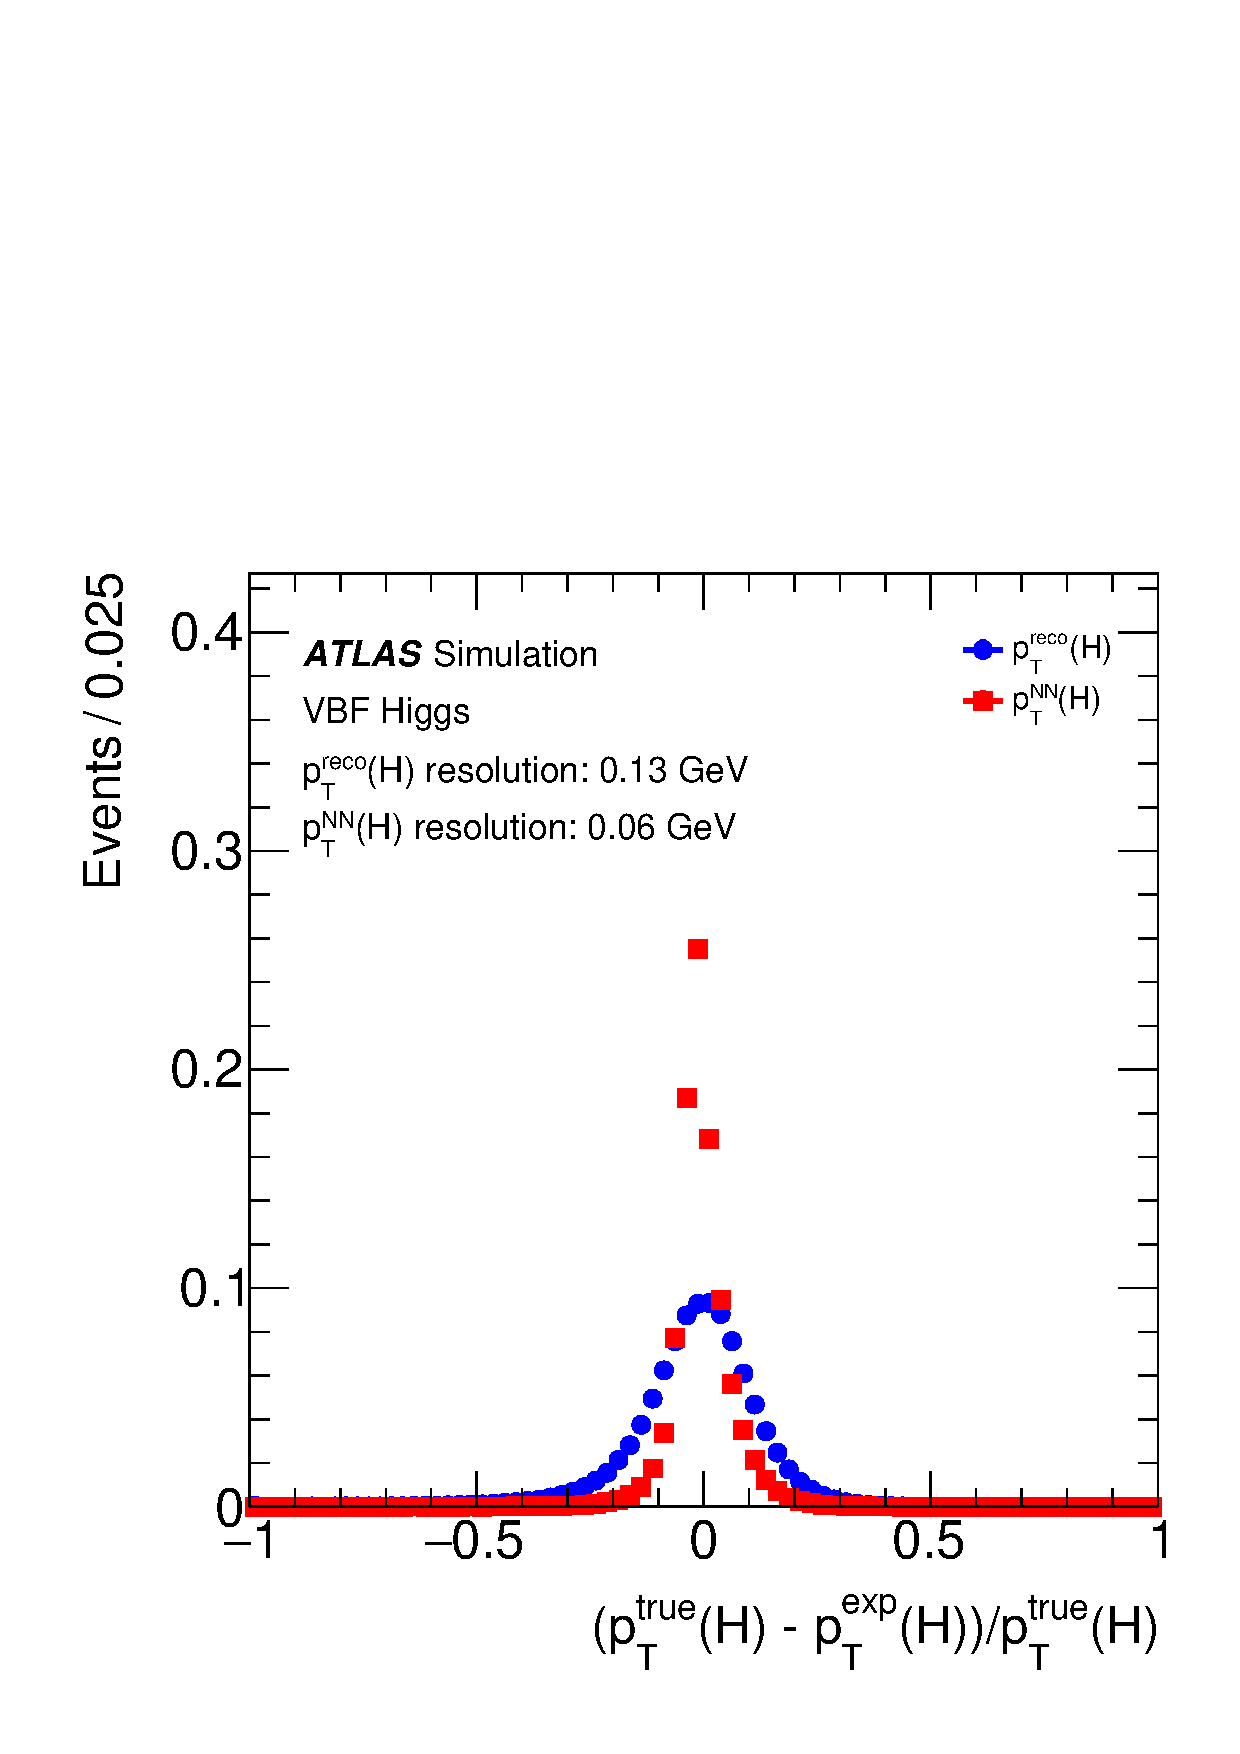
\includegraphics[width=0.55\textwidth]{NN_1.pdf}
    \caption{Resolution of $p_{\text{T}}^{H}$ with respect to truth simulation, comparing the reconstruction from the sum of the $\tau$-lepton four-momenta and \etmiss with the NN-based regression for simulated VBF Higgs boson events~\cite{differential_htautau}.}
    \label{fig:ptH_resolution}
\end{figure}

%%%%%%%%%%%%%%%%%%%%%%%%%%%%%%%%%%%%%%%%%%%%%%%%%%%%%%%%%%%%%%%%%%%%%%%%%%%%%%%%%%%%%%%%%%%%%%%%%%%%%%%%%%%%%%%%%%%%%%%%%%%%%%%%%%%%%%%%%%%%%%%%%%%%%%%%%%%%%%%%%%%%%%%%%%%%%%%%%%%%
\section{Event classification and background definition}
\label{sec:event_selection_background}

The event selection in the \htautau\ analysis can be regarded as a two-stage procedure. 
After the channel classification (\tauemu, \taulephad, \tauhadhad), each channel is further classified into event categories specifically designed to isolate a given Higgs boson production mode considered as signal. 
The goal is to maximize the sensitivity to the SM Higgs boson signal, while ensuring a robust estimation of the Higgs observables reconstructed from the $\tau$-leptons, and to match as closely as possible the phase space binning defined by the STXS framework.

In \ttHtt, the selection requires exactly two reconstructed $\tau_{\text{had-vis}}$ objects, with the \pt requirements detailed in Section~\ref{sec:object_definiton}. 
Additional requirements are applied to suppress background contributions, particularly at low-$p_{\text{T}}$: the angular separation between the two $\tau_{\text{had-vis}}$ candidates is required to satisfy $\Delta R > 0.6$ in order to avoid overlaps, and at least one additional central jet ($|\eta| < 3.2$) with $p_{\text{T}} > 70$~GeV is required, which reduces the contribution from dijet background processes.

Furthermore, the two $\tau_{\text{had-vis}}$ candidates are required to have opposite electric charge. 
Unlike other production modes considered in the \htautau\ analysis, at least one $b$-jet is requiered, as $b$-jets are expected from the top-quark decays produced together with the Higgs boson in \ttH\. 
Finally, to enhance the reconstruction efficiency of the invariant mass of the system, additional requirements are imposed on the missing transverse momentum \etmiss and on the visible momentum fractions of the $\tau$-leptons ($x_0$ and $x_1$). 
All selection requirements, hereafter referred to as preselection or \ttH preselection requirements, are summarised in Table~\ref{tab:tth_hadhad_selection}.

\begin{table}[htbp]
    \centering
    \caption{Summary of the event selection for the $\tau_{\text{had}}\tau_{\text{had}}$ channel and the dedicated $t\bar{t}(0\ell)H \to \tau_{\text{had}}\tau_{\text{had}}$ category.}
    \renewcommand{\arraystretch}{1.6} % más espacio vertical
    \scriptsize % letra un poco más pequeña
    \begin{tabular}{l c}
    \hline
    \textbf{Preselection} & $\tau_{\text{had}}\tau_{\text{had}}$ \\
    \hline
    Object counting & \# of $e/\mu = 0$, \# of $\tau_{\text{had-vis}} = 2$ \\
    $p_{\text{T}}$ cut & $\tau_{\text{had-vis}}$: $p_{\text{T}} > 40, 30$~GeV \\
    Identification & $\tau_{\text{had-vis}}$: RNN Medium \\
    Charge product & Opposite charge \\
    $b$-tagging & DL1r 70\%
    \etmiss & \etmiss $> 20$~GeV \\
    Leading jet & $p_{\text{T}} > 70$~GeV, $|\eta| < 3.2$ \\
    Angular & $0.6 < \Delta R_{\tau_{\text{had-vis}}\tau_{\text{had-vis}}} < 2.5$, 
               $|\Delta\eta_{\tau_{\text{had-vis}}\tau_{\text{had-vis}}}| < 1.5$ \\
    Coll. app. $x_1, x_2$ & $0.1 < x_1 < 1.4$, $0.1 < x_2 < 1.4$ \\
    \hline
    \end{tabular}
    
    \vspace{0.6cm}
    
    \begin{tabular}{l c}
    \hline
    \textbf{Category} & $\tau_{\text{had}}\tau_{\text{had}}$ \\
    \hline
    $t\bar{t}(0\ell)H \to \tau_{\text{had}}\tau_{\text{had}}$ & 
    \# of jets $\geq 6$ and \# of $b$-jets $\geq 1$ \\
    & or \# of jets $\geq 5$ and \# of $b$-jets $\geq 2$ \\
    \hline
    \end{tabular}
    
    \label{tab:tth_hadhad_selection}
    \end{table}
    
The prerequisites described above apply mainly to the \tauhadhad channel. 
For the \ttH\ production mode under study, the final state is further characterized by the presence of six jets, two of which are expected to be tagged as $b$-jets, as illustrated in Fig.~\ref{fig:tth_topo}. 

To increase the signal acceptance, this selection is slightly relaxed. Events with four or fewer jets are dominated by background, while a significant fraction of the signal appears in events with at least five jets. 
Given the large background contribution observed in events with exactly five jets and only one $b$-jet, the final requirement is defined as either more than five jets with at least two $b$-tags, or more than six jets with at least one $b$-tag.

\begin{figure}[htbp]
    \centering
    \begin{subfigure}[b]{0.48\textwidth}
        \centering
        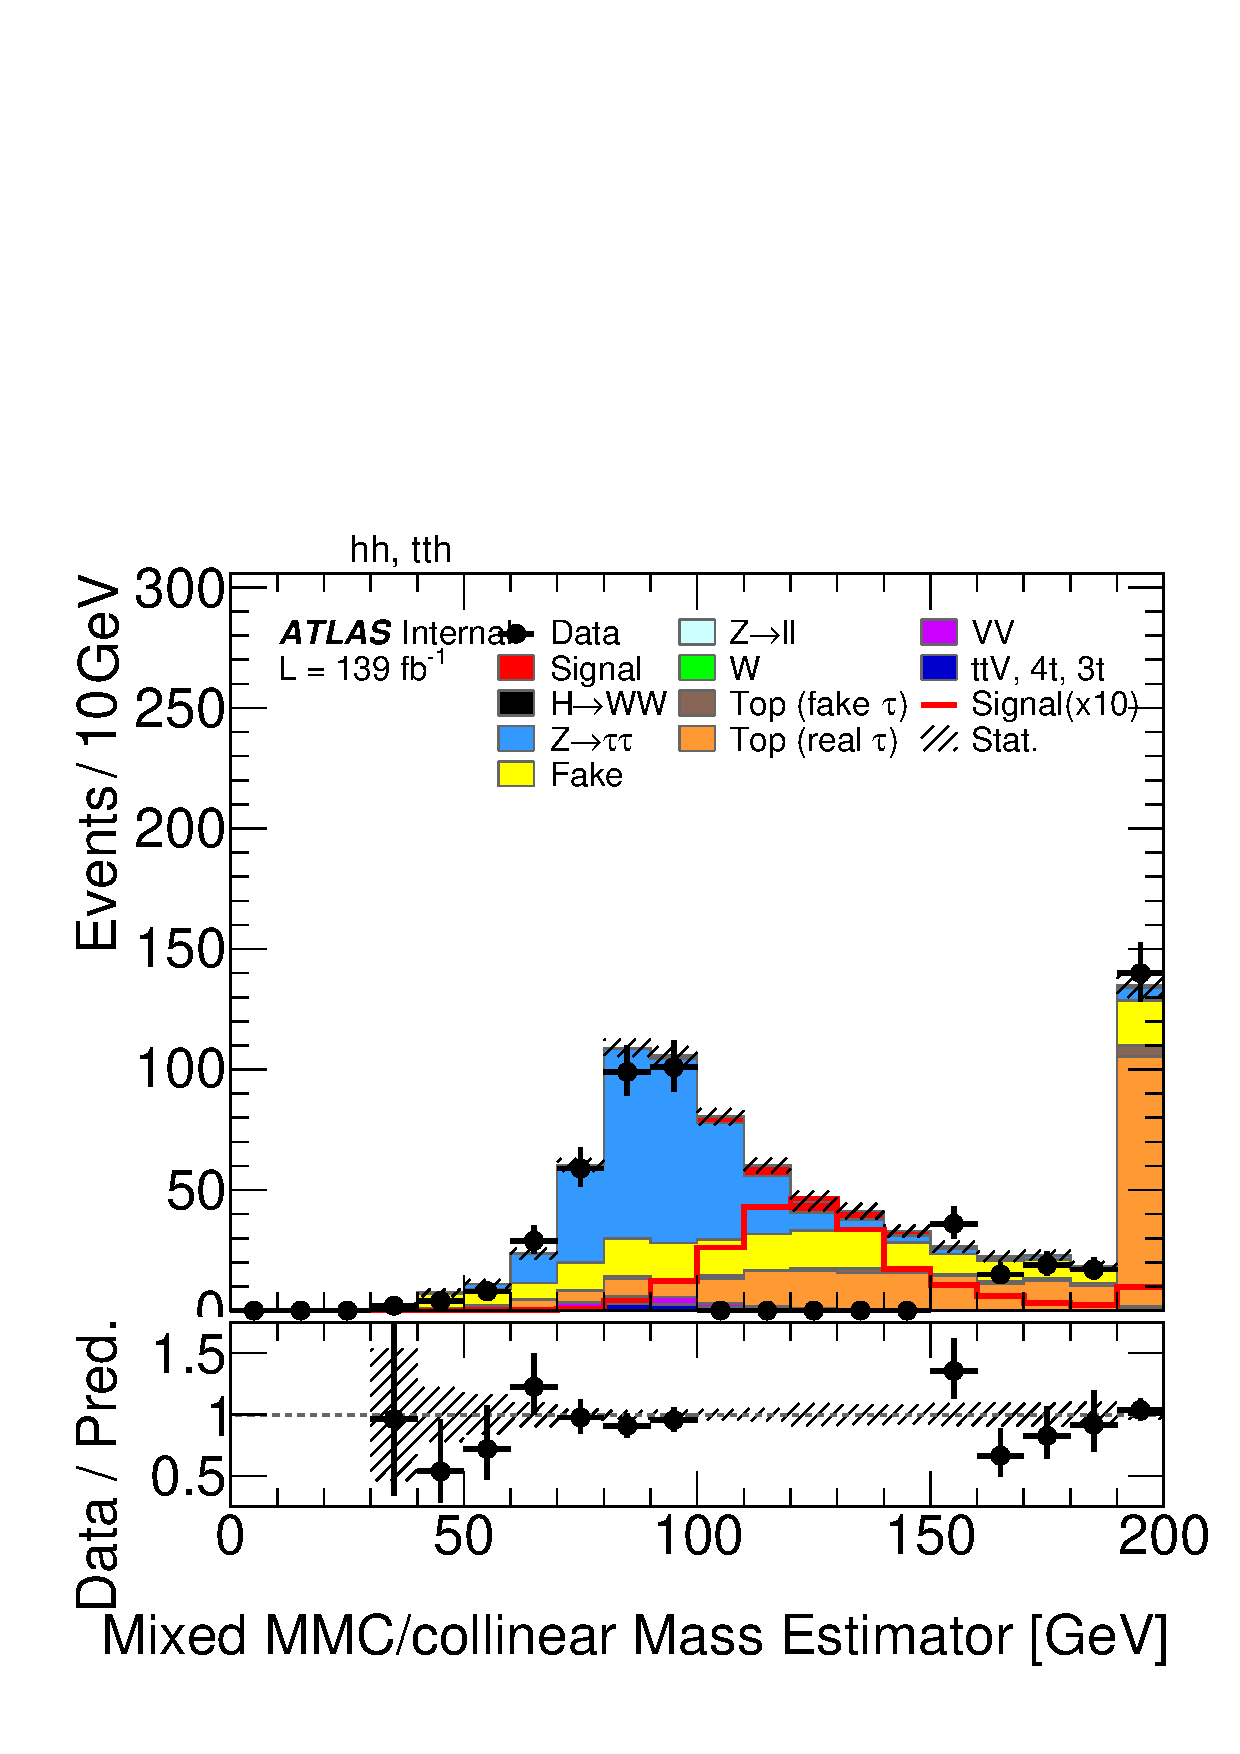
\includegraphics[width=\textwidth]{plot_ditau_mmc_mlm_m_fix_hh_tth.pdf}
        \caption{}
        \label{reconstructed_preselection_a}
    \end{subfigure}
    \hfill
    \begin{subfigure}[b]{0.48\textwidth}
        \centering
        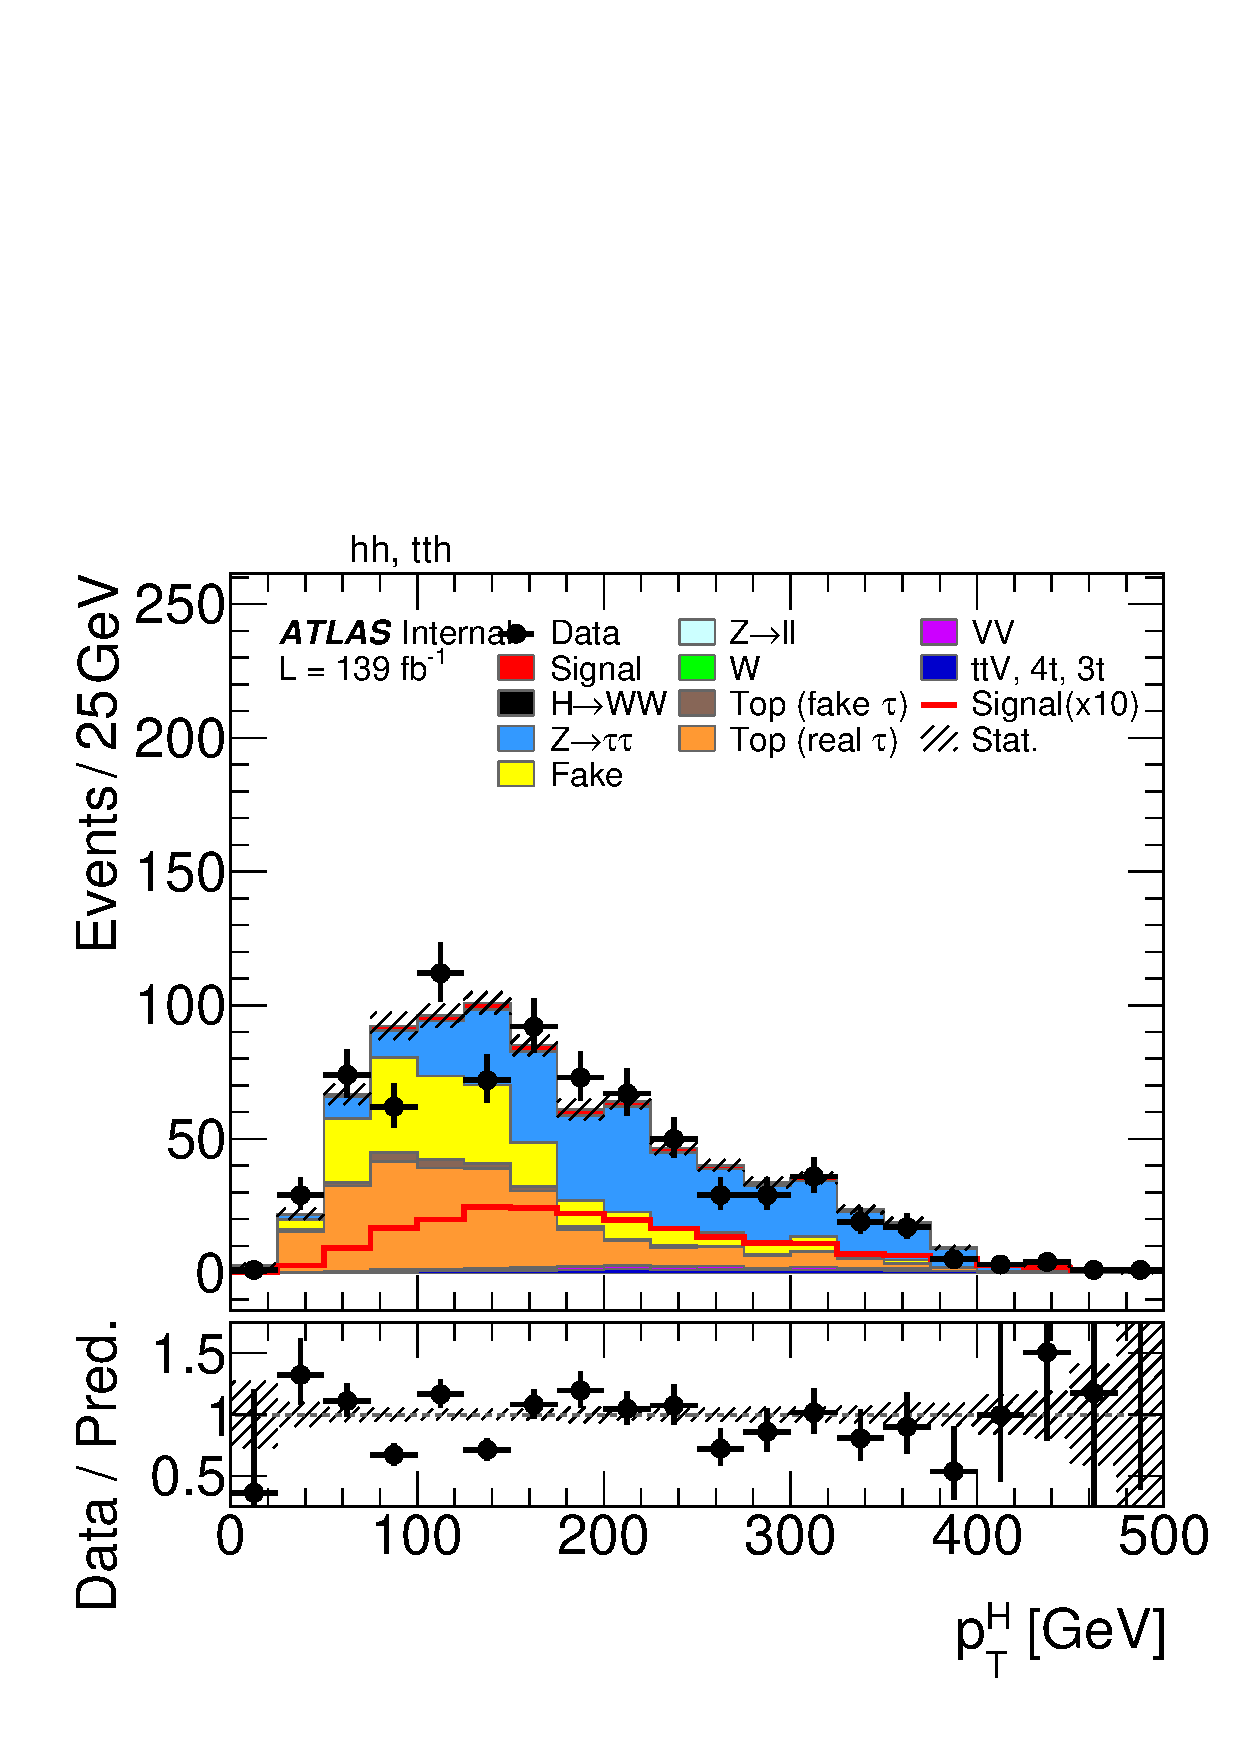
\includegraphics[width=\textwidth]{plot_ditau_pt_NN_kin_hh_tth.pdf}
        \caption{}
        \label{reconstructed_preselection_b}
    \end{subfigure}
    \caption{Distributions of (a) the Higgs boson mass, reconstructed with the mixed MMC/collinear estimator with the range $100-150$~GeV blinded, and (b) the Higgs transverse momentum $p_{\text{T}}^H$, shown at the $t\bar{t}H$ preselection level. Only statistical uncertainties are included.}
    \label{reconstructed_preselection}
\end{figure}


Figure~\ref{reconstructed_preselection} shows the reconstructed Higgs boson candidate mass and \pth distributions in data and MC simulation after applying the preselection. 
From the invariant mass distribution in Fig.~\ref{reconstructed_preselection_a}, the main backgrounds affecting the analysis can be clearly identified. 
Already with this single variable, a first signal-to-background discrimination can be achieved by defining appropriate cuts. 

The dominant background arises from \ztautau$+$jets events, which peak below the Higgs boson signal, around the $Z$ boson mass of 90~GeV. 
A flatter contribution comes from \ttbar production, since the $\tau$ leptons originate from different particles. 
These events populate the high-mass tail, reflecting the higher energy scale of the process. In addition, a non-negligible contribution is given by fakes backgrounds from QCD multijet events where one or two jets are misidentified as \tauhad candidates. 

After applying the preselection, the expected yields are $309.0 \pm 5.6$ \ztautau events, $266.3 \pm 6.7$ \ttbar events, $184.5 \pm 8.6$ fakes, and $19.5 \pm 0.3$ \ttHtt signal events (all uncertainties statistical only). The \mmc variable therefore allows the definition of three regions:
\begin{itemize}
    \small
    \item Higgs $\mmc$ window ($100~\text{GeV} < \mmc < 150~\text{GeV}$): Signal enhanced region.
    \item High $\mmc$ sideband ($\mmc > 150~\text{GeV}$): Dominated by $t\bar{t}$ events.
    \item Low $\mmc$ sideband ($0 < \mmc < 100~\text{GeV}$): Dominated by $Z(\tau\tau)$ production, since its distribution will peak around the $Z$ boson mass.
\end{itemize}

In practice, the final categorization of events into multiple signal and control regions targeting the different STXS bins is not performed using the \mmc variable, since its distribution is exploited directly in the likelihood fit used to extract the signal, as discussed in Section~\ref{sec:statistical_tth}. 
Instead, dedicated multivariate discriminants are trained to enhance the signal contribution over the backgrounds in specific signal regions and to define control regions that constrain and validate the background components in the final statistical fit. 
Further details on these classifiers are provided in Section~\ref{sec:tth_mva}.  

Regarding the estimation of the main backgrounds in the \ttHtt analysis, as explained in Section~\ref{sec:analysis_strategy},
the dominant background arises from \ztautau+jets processes, contributing more than $40\%$ of the total background yield. 
These events are modeled with the MC simulations described in Section~\ref{subsec:higgs_mc}, and their modeling and normalization are validated against data in dedicated control regions enriched in this background, defined using the MVA discriminants as detailed in Section~\ref{sec:tth_categories}. 
Similarly, \ttbar production is modeled with MC and validated in data using dedicated control regions within the analysis phase space.

The third major background contribution comes from fakes, i.e.\ multijet events in which one or two jets are misidentified as \tauhadvis candidates. 
This background is estimated with a data-driven fake-factor method~\cite{fakes_paper}. 
The contribution of fakes to the signal regions is derived from dedicated control regions, one of which is the anti-ID region, where one of the \tauhad candidates fails the Medium identification WP but passes the Loose WP, such that the event is still kept in the derivations~\footnote{``Derivations'' denote datasets containing MC simulations or data that have already been processed, with certain selection and trigger requirements applied to reduce their size and make them more manageable for the analyses.} datasets used. 
In this region, a template for the fake contribution is obtained by subtracting simulated prompt-\tauhadvis backgrounds from the data distribution. 
This template is then scaled by a transfer factor, the fake factor (FF), correcting for the different selection efficiencies between \tauhadvis candidates passing or failing the Medium selection.

Two sets of FFs are used, derived in $W$+jets control regions of the \taulephad channel enriched in jets faking \tauhadvis.
The need for two sets arises because, as mentioned, the analysis derivations do not contain events without at least Loose \tauhadvis candidates, so FFs are combined from regions defined with a Loose requirement and from regions without it.

The FFs are therefore computed in three distinct regions for the two sets under consideration, differing only in the applied identification requirement. 
In both cases, the numerator is given by the number of data events in the $W$+jets CR with the Medium WP applied. In order to define this CR, the further cuts are applied:
\begin{itemize}
  \small
  \item Matching of the \tauhadvis candidate to the \texttt{tau25\_medium1\_tracktwo(EF)} trigger
  \item Leading jet \pt cut kept at 20~GeV in order to increase the sample size
  \item Requiring $\Delta\eta(\ell,\tau_{\text{had-vis}}) > 0.6$ in order to remove overlap
\end{itemize}
On the other hand, the denominator corresponds to the anti-\tauhadvis region, defined by inverting the requirement in the not-medium (nm) case, or by requiring at least the Loose WP in the loose-not-medium (lnm) case. 
Events with genuine \tauhadvis are subtracted in all regions using MC simulation. 
The resulting FFs, which encapsulate the probability for jets faking \tauhadvis to pass the identification relative to those rejected, are thus defined as:
\begin{align}
    FF_{nm} &= 
    \frac{(\text{Data} - \text{MC})^{\text{WCR}}_{\text{medium } \tau_{\text{had-vis}}}}
         {(\text{Data} - \text{MC})^{\text{WCR}}_{\text{not-medium } \tau_{\text{had-vis}}}}, \nonumber \\[6pt]
    FF_{lnm} &= 
    \frac{(\text{Data} - \text{MC})^{\text{WCR}}_{\text{medium } \tau_{\text{had-vis}}}}
         {(\text{Data} - \text{MC})^{\text{WCR}}_{\text{loose-not-medium } \tau_{\text{had-vis}}}},
\label{eq_fakes}
\end{align}
where fake factors are derived in bins of \pt and $|\eta|$ of the \tauhadvis candidates, as they exhibit a significant dependence on these variables. 
Ultimately, the smaller the FFs, the better the performance of the \tauhad identification algorithm, since this indicates a lower probability for jets to mimic \tauhadvis candidates.

The estimation of the fake background is obtained by weighting the \tauhadhad anti-ID events with the corresponding FFs, which provides the predicted number of jets misidentified as \tauhadvis in the signal region. 
The set of regions used for the application of FFs depends on the identification criteria adopted. 
Further details on the FF application can be found in earlier rounds of the \Htautau analysis~\cite{couplings} and in Chapter~\ref{chap:run3_tth}, where a direct contribution was made to the re-estimation of fakes using the rel.22 Run-2 and Run-3 data, including the implementation of new $\tau$-lepton identification techniques.  

Although the full discussion of systematic uncertainties is deferred to Section~\ref{sec:tth_systematics}, here the specific uncertainties associated with the estimation of this background are introduced, which are evaluated through three types of variations. 
The differences observed with respect to the nominal procedure are taken as the systematic uncertainty assigned to the fake background estimate.  

The first group corresponds to the statistical uncertainties of the fake factors derived in the $W+$jets CRs.  
These are evaluated by varying the fake factors within one standard deviation of their statistical uncertainty.
Independent variations are assigned for 1-prong and 3-prong \tauhadvis candidates, and for the \textit{nm} and \textit{lnm} categories, resulting in four separate uncertainties.  

The second group addresses potential differences in the background composition between the regions where the fake factors are measured and those where they are applied.  
Since the relative fractions of light-quark, gluon, and heavy-flavour jets may vary significantly, dedicated CRs enriched in fake $\tau$ candidates are used to evaluate this effect.  
In addition to the nominal \taulephad $W+$jets CR, alternative \tauhadhad regions are considered: one defined by the separation $\Delta\eta(\tauhadvis,\tauhadvis)$ and another based on same-sign events.  
Fake factors are re-derived in these regions, and the full background estimation procedure is repeated to compare the results with the nominal prediction.  

The third group concerns the parametrization strategy of the FFs.  
To evaluate this effect, FFs are recalculated in the \tauhadhad same-sign region using coarser binning to ensure sufficient statistics.  
Separate values for leading and subleading \tauhadvis candidates are obtained and then combined to reproduce the nominal parametrization, since the \taulephad $W+$jets CR does not allow them to be distinguished.  
These same-sign fake factors are subsequently applied to the anti-ID region to perform closure tests.  
The $m_{\tau\tau}^{\text{MMC}}$ distribution is used for this purpose, and the ratio of prediction to data is taken as an additional weight on fake events, thereby defining the associated systematic uncertainty.  

%%%%%%%%%%%%%%%%%%%%%%%%%%%%%%%%%%%%%%%%%%%%%%%%%%%%%%%%%%%%%%%%%%%%%%%%%%%%%%%%%%%%%%%%%%%%%%%%%%%%%%%%%%%%%%%%%%%%%%%%%%%%%%%%%%%%%%%%%%%%%%%%%%%%%%%%%%%%%%%%%%%%%%%%%%%%%%%%%%%%
\section{MVA strategy for \ttHtt}
\label{sec:tth_mva}

Beyond the event selection described in the previous section, the events are further divided into categories designed to optimise the signal-to-background separation, thereby increasing both sensitivity and purity, as will be detailed in Section~\ref{sec:tth_categories}. This categorisation relies on ML techniques, in particular on the use of BDTs introduced in Section~\ref{sec:bdt_general}, to enhance the separation of \ttH signal events from the dominant \ztautau and \ttbar backgrounds.

This strategy improves over the approach adopted in the previous round of this \htautau analysis~\cite{couplings}, where two binary BDTs were trained independently to separate \ttH from \ztautau and \ttH from \ttbar, respectively. The outputs of the two discriminants were then combined by applying selection cuts to define the analysis categories. 

In this work, the strategy of using two independent binary classifiers has been replaced by a multiclass BDT, trained to simultaneously distinguish between \ttH, \ztautau and \ttbar events. The output of this classifier consists of three scores, each associated with one event class, and normalised to fulfil the condition $BDT_{\text{\ttH}} + BDT_{\text{Z}} + BDT_{\text{\ttbar}} = 1$.
The training employs MC simulated events of the three processes, following the procedure described in Section~\ref{subsec:higgs_mc}. In addition, the available statistics of the nominal \ttbar samples, produced with \textsc{powheg+pythia}, are enhanced with alternative samples with modified top-quark masses derived with \textsc{madgraph5}\_a\textsc{mc@nlo} and additional fast simulated samples.

The choice of a multiclass classifier suits particularly well when the classes to be separated are correlated and when the characteristic observables used as inputs are themselves related. This is indeed the case here, as the previous independent binary trainings were largely driven by jet-related features in the final state or by properties of the two \tauhadvis candidates. In such situations, where binary BDTs rely on similar and correlated input variables, the adoption of a multiclass approach can provide an advantage.

\subsection{Multiclass BDT setup}
\label{setup_bdt}
Before presenting the details of the BDT setup, it should be noted that the MC event selection used for the training relies solely on the preselection described in Section~\ref{sec:event_selection_background}. The BDT is trained to distinguish among three event classes, corresponding to the three processes under study. The algorithm is defined and trained using the \textsc{tmva} package of the \textsc{root} framework, as mentioned in Section~\ref{sec:bdt_general}. In that section it is also described the decision tree structure, the choice of hyperparameters, and the additional methods defining the training procedure. The settings that were used are briefly summarised below.
\begin{itemize}
    \small
    \item Number of trees: 1000
    \item Minimum node size: 2.5\%
    \item Maximum depth of a tree: 2
    \item Boosting algorithm used: Grad
    \item Bagging is used with bagged sample fraction of 0.2~\footnote{Bagging is a resampling technique that is commonly used, in which a classifier is repeatedly trained using resampled training
    events such that the final classifier is an average representation of each individual classifier.}
    \item Number of cuts on the variables: 20
\end{itemize}
These hyperparameters were chosen as they provided the best performance, with no significant improvement observed from further optimisation. In order to enhance the sensitivity and to maximise the use of the available statistics, a five-fold cross-validation procedure is also implemented, ensuring that all events are employed for both training and testing.

\subsection{Input variable selection}

Most of the variables used in the training of the multiclass BDT result from merging those already employed in the two previous binary BDT trainings, many of which were common to both. These variables will be detailed below, but it is worth starting by highlighting the new observables included in this work.

The first of these is the minimum angular distance between any pair of jets in the event, $\Delta R^{\text{min}}_{jj}$. This variable helps for discriminating \ttbar from the signal and from \ztautau, since jet pairs in top-antitop production tend to be more widely separated. A related quantity is the minimum distance between a reconstructed \tauhad and a $b$-tagged jet, $\Delta R^{\text{min}}_{(\tau,b\text{-jet})}$. In this case, while in the \ttbar background both \tauhad originate from top-quark decays, in the \ttH signal the $\tau$-leptons come from the Higgs boson. Consequently, the angular separation between a \tauhad and a $b$-jet, considering all possible combinations, carries discriminating power. 

In addition, and primarily with the aim of further improving the classification of \ttbar events, further angular observables associated with jets in the final state are included. Specifically, the pseudorapidity of up to the five leading jets is added to the input set.

Finally, in order to enhance the discrimination against \ztautau events, we exploit the fact that the jets produced in this process exhibit non-trivial correlations. As discussed in Ref.~\cite{ztt_jets}, jets in $Z+\text{jets}$ events mainly originate from QCD radiation, which results in characteristic patterns in their transverse momenta. In contrast, in \ttH events jets predominantly arise from top-quark decays and from the hard matrix element. As a consequence, consecutive jets in the $Z+\text{jets}$ background tend to preserve similar $p_{\text{T}}$ ratios, yielding a roughly flat cross-section distribution as a function of these ratios. This observation motivates the inclusion of jet $p_{\text{T}}$ ratios as discriminating variables for the BDT.  
Several possibilities were explored, such as jet multiplicities above various $p_{\text{T}}$ thresholds and different combinations of $p_{\text{T}}$ ratios up to the fourth leading jet. However, due to strong correlations among them and with already included observables, only three ratios with the highest separation power between signal and background were used:
\begin{itemize}
    \small
    \item \textbf{ratio01} : \pt($\text{jet}_1$)/\pt($\text{jet}_0$),
    \item \textbf{ratio12} : \pt($\text{jet}_2$)/\pt($\text{jet}_1$),
    \item \textbf{ratio13} : \pt($\text{jet}_3$)/\pt($\text{jet}_1$),
\end{itemize}
where $\text{jet}_0$ denotes the leading jet, $\text{jet}_1$ denotes the subleading jet, etc.

The complete list of input variables is listed in Table~\ref{tab:ttH_variables}, and can be grouped into four main categories:  
\begin{itemize}
    \item Jet system properties: as already mentioned, variables such as the jet pseudorapidities are complemented with quantities related to their transverse momenta. These include $H^{\text{jets}}_{\text{T}}$, defined as the scalar sum of the transverse momenta of all jets in the event, and \texttt{SumPtBjet} for the case of $b$-tagged jets. Variables associated with the reconstruction of the top quark are also included in this category, since they involve particles present in the signal process. A $W$-boson candidate, $m^{\text{best}}_{W}$, is reconstructed from pairs of non-$b$-tagged jets by selecting the combination with invariant mass closest to the nominal $W$ mass. This $W$ candidate is then combined with a $b$-tagged jet to build top-quark candidates, with $m^{\text{top}}_{W_{\text{best}}}$ defined as the invariant mass of the candidate lying closest to the expected top-quark mass.
    \item Properties of $\tau$-leptons: variables describing both \tauhad candidates in the final state are included, such as the transverse momentum of the sub-leading \tauhad, $p^{\tau_1}_{\text{T}}$, and the pseudorapidity of the leading one, $\eta_{\tau_0}$. The transverse momentum of the di-$\tau$ system is also considered, since its properties differ significantly across the three processes under study.
    \item Angular distances: a set of variables related to angular separations between objects in the event are included. These comprise the pseudorapidity difference of the two $\tau$ candidates, $\Delta\eta(\tau_0,\tau_1)$, as well as their angular distance $\Delta R(\tau_0,\tau_1)$. The previously introduced minimum angular distances between jets, and between a $b$-tagged jet and a \tauhad candidate, are also considered.
    \item \etmiss description: two additional variables are added to characterise the missing transverse energy, namely the total \etmiss itself and the minimum azimuthal angle between $\vec{E}^{\text{miss}}_{\text{T}}$ and a \tauhad.
\end{itemize}

It should be emphasised that the \mmc, although highly discriminating, is not included as part of the training. Instead, it is used directly in the binned likelihood fit employed to extract the signal. If it were included at the event-selection level of the training (for instance by restricting events to the Higgs boson mass window), a large fraction of the background statistics would be removed, which is not desirable. Moreover, if introduced as an input to the BDT, the classifier would be biased to produce a peak around $125$~GeV also for the background processes, thereby degrading its discriminating power.

\begin{table}[h]
    \small
    \centering
    \caption{Variables used in the multivariate tagger for the $t\bar{t}H$ analysis.}
    \renewcommand{\arraystretch}{1.3}
    \setlength{\tabcolsep}{10pt}
    \begin{tabular}{p{2cm} p{8cm}}
      \toprule
      \textbf{Group} & \textbf{Variable} \\
      \midrule

      \multirow{9}{*}{\rotatebox{90}{Jet properties}} 
      & Invariant mass of the two leading jets $p_{\text{T}}(jj)$ \\
      & Product of $\eta$ of the two leading jets \\
      & Sub-leading jet $p_{\text{T}}$ \\
      & $\eta$ of the 5 leading jets \\
      & Scalar sum of all jets $p_{\text{T}}$ \\
      & Scalar sum of all $b$-tagged jets $p_{\text{T}}$ \\
      & Best $W$-candidate dijet invariant mass \\
      & Best top-quark-candidate three-jet invariant mass \\
      & Ratio of the $p_{\text{T}}$ of jet pairs \\
      \midrule

      \multirow{6}{*}{\rotatebox{90}{Angular distances}} 
      & $\Delta\phi$ between the two leading jets \\
      & $\Delta\eta$ between the two leading jets \\
      & Minimum $\Delta R$ between two jets \\
      & Minimum $\Delta R$ between a $b$-tagged jet and a $\tau$ \\
      & $|\Delta\eta(\tau,\tau)|$ \\
      & $\Delta R(\tau,\tau)$ \\
      \midrule

      \multirow{3}{*}{\rotatebox{90}{$\tau$-lepton}} 
      & $p_{\text{T}}(\tau)$ \\
      & Sub-leading $\tau$ $p_{\text{T}}$ \\
      & Leading $\tau$ $\eta$ \\
      \midrule

      \multirow{2}{*}{\rotatebox{90}{\etmiss}} 
      & Missing transverse momentum $E_{T}^{\text{miss}}$ \\
      & Smallest $\Delta\phi(\tau, \vec{E}_{T}^{\text{miss}})$ \\
      \bottomrule
    \end{tabular}
    \label{tab:ttH_variables}
\end{table}

Figures~\ref{tth_vars_tmva_1} and~\ref{tth_vars_tmva_2} show the distributions of all input variables used for each of the event classes. As already anticipated, these distributions provide a direct indication of which variables are expected to be most discriminating and therefore most effectively exploited by the BDT. Characteristic observables of the di-$\tau$ system exhibit markedly different shapes across the three processes, such as the pseudorapidity difference or the transverse momentum of the system. Jet-related quantities are also highly valuable, in particular the pseudorapidity of the leading and sub-leading jets, as well as their transverse momentum ratio.

\begin{figure}[htbp]
    \centering
    % Primera figura
    \begin{subfigure}{0.95\linewidth}
      \centering
      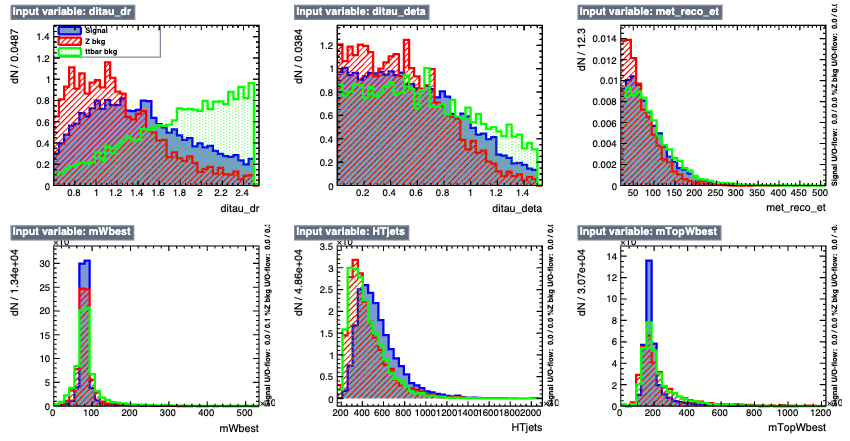
\includegraphics[width=\linewidth]{new_vars_1}
    \end{subfigure}
    \vspace{0.5cm} % Espacio vertical entre las dos
    % Segunda figura
    \begin{subfigure}{0.95\linewidth}
      \centering
      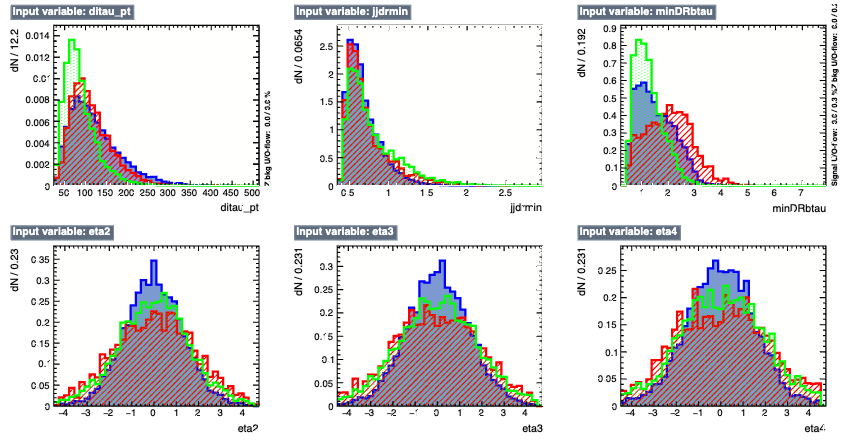
\includegraphics[width=\linewidth]{new_vars_2}
    \end{subfigure}
    \caption{Distribution of the input variables used for the multiclass BDT training for \ttHtt, evaluated on Signal (blue), \ztautau background (red) and \ttbar background (green) events.}
    \label{tth_vars_tmva_1}
  \end{figure}

  \begin{figure}[htbp]
    \centering
    % Primera figura
    \begin{subfigure}{0.95\linewidth}
      \centering
      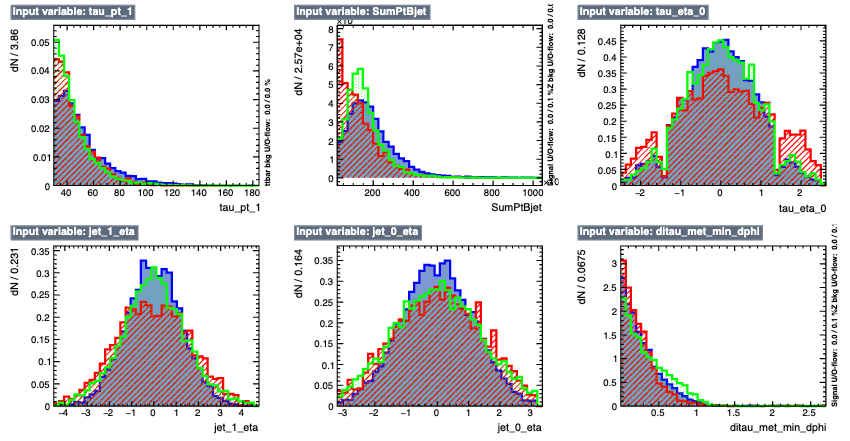
\includegraphics[width=\linewidth]{new_vars_3}
    \end{subfigure}
    \vspace{0.5cm} % Espacio vertical entre las dos
    % Segunda figura
    \begin{subfigure}{0.95\linewidth}
      \centering
      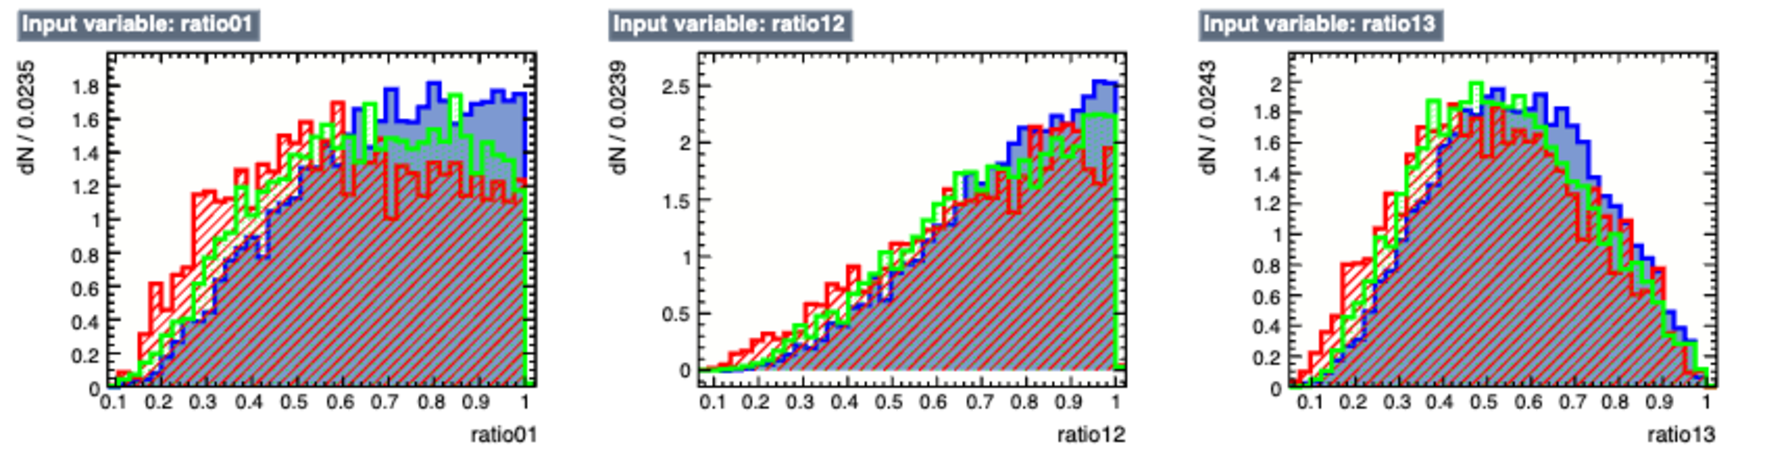
\includegraphics[width=\linewidth]{new_vars_4}
    \end{subfigure}
    \caption{Distribution of the input variables used for the multiclass BDT training for \ttHtt, evaluated on Signal (blue), \ztautau background (red) and \ttbar background (green) events.}
    \label{tth_vars_tmva_2}
  \end{figure}


  It is also important to monitor the correlation coefficients among the input variables for the three processes considered, which are shown in Figure~\ref{tth_vars_corr}.
  \begin{figure}[htbp]
    \centering
    \setlength{\tabcolsep}{2pt}
    \renewcommand{\arraystretch}{0}
  
    \begin{tabular}{@{}c c@{}}
      \multicolumn{2}{c}{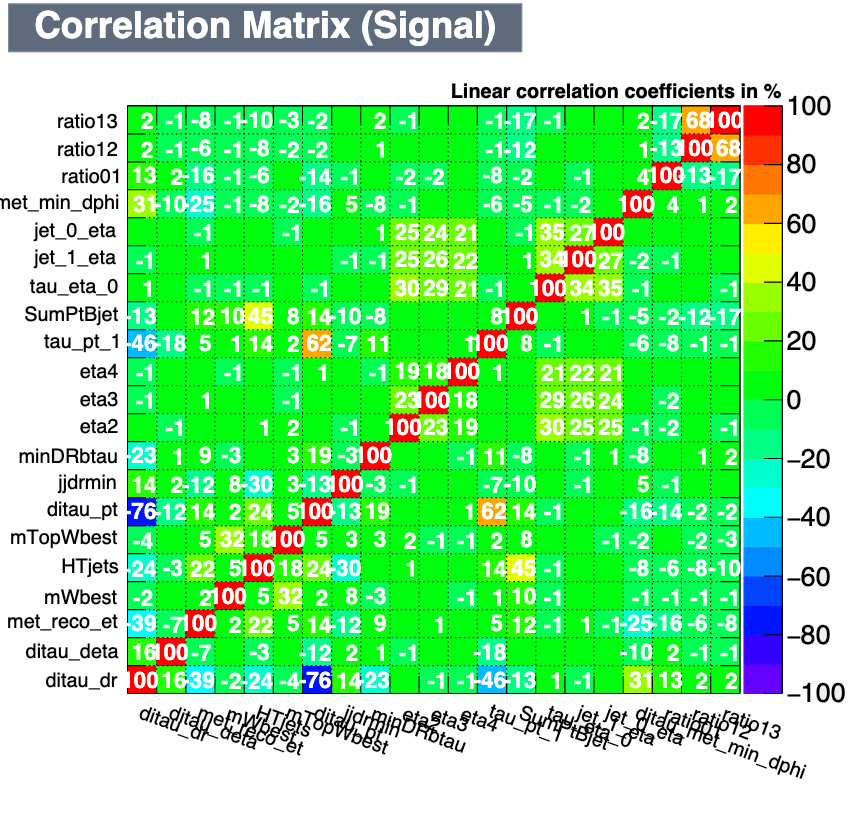
\includegraphics[width=0.48\textwidth]{corr_signal}} \\[6pt]
      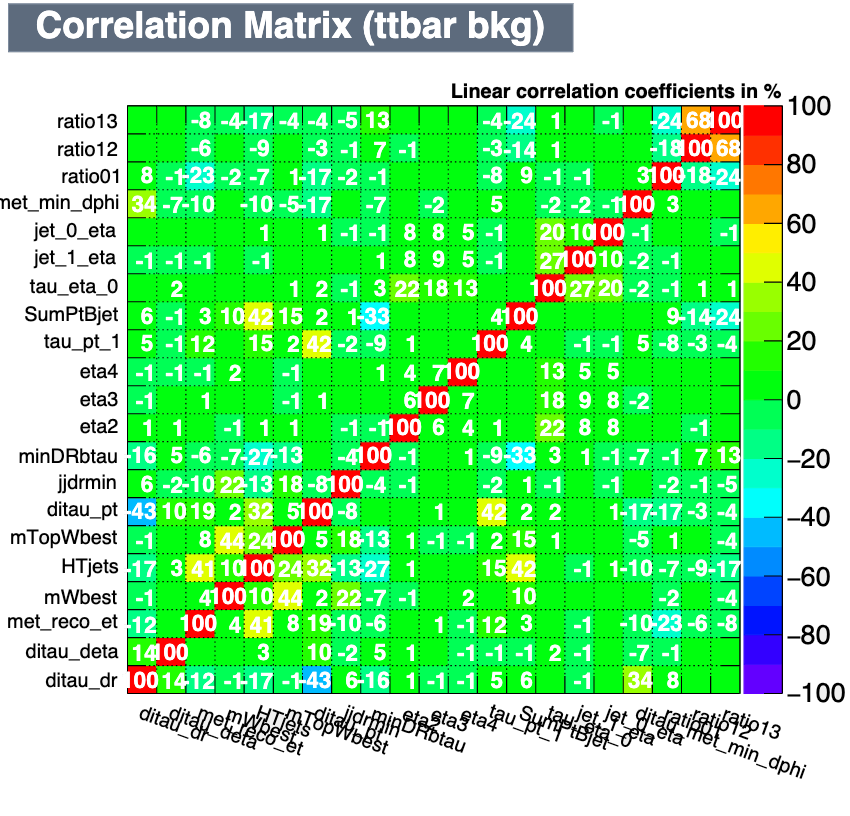
\includegraphics[width=0.48\textwidth]{corr_ttbar} &
      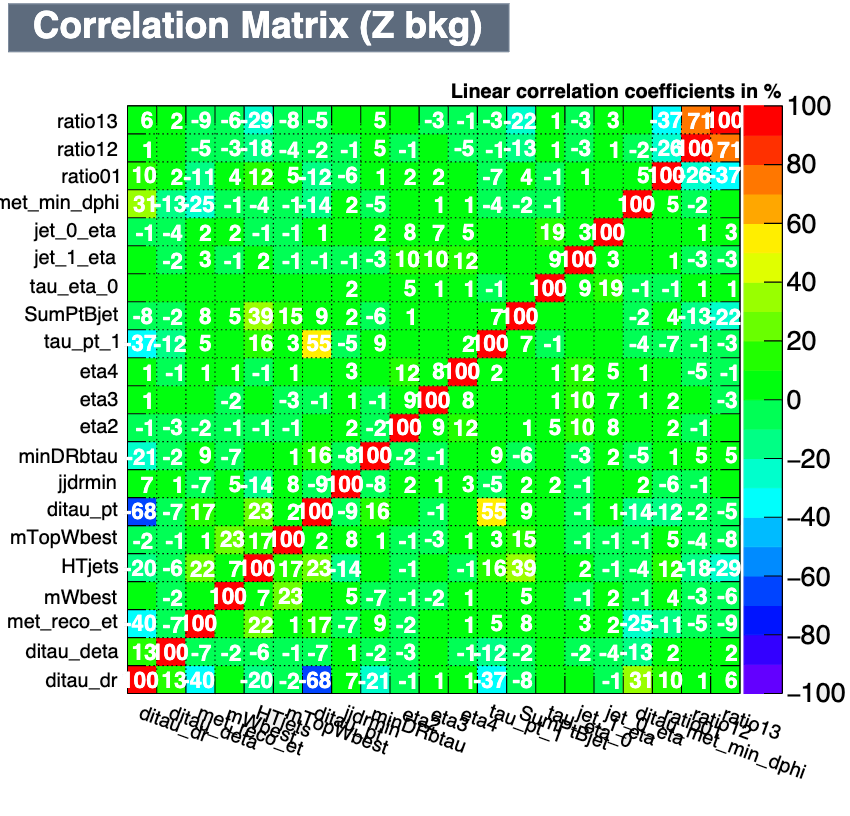
\includegraphics[width=0.48\textwidth]{corr_Z}
    \end{tabular}
  
    \caption{Correlation coefficients among the variables used to train the multiclass BDT for signal (top), \ttbar (bottom left) and \ztautau (bottom right). All events at preselection level are included.}
    \label{tth_vars_corr}
  \end{figure}
  
  As can be seen, the chosen variables are not excessively correlated with each other, and for some of them the correlation coefficients vary depending on the process. This is the case, for instance, for the transverse momentum and the angular distance of the two \tauhad candidates, or for the pseudorapidity of the leading jets with respect to that of the leading \tauhad. Other variables show comparable correlations across the three processes, yet the selected set was found to provide the best performance in the final categorisation, rather than excluding any of them.
  

\subsubsection*{Data-MC modelling}

Beyond evaluating the discriminating power of the variables to justify their inclusion in the training, it is equally important to verify that they are accurately modelled in the MC simulations employed. This is not always trivial, particularly in such restricted and selective regions of phase space as those considered in this analysis. Since the discriminant trained on these simulations will be applied to real collision data, it is essential to guarantee a proper data/MC agreement.  

Figures~\ref{tth_vars_modelling_1}-\ref{tth_vars_modelling_3} illustrate the good data/MC agreement observed for the input variables, by comparing their distributions across all relevant processes in the channel at the \ttH preselection level.

\begin{figure}[htbp]
    \centering
    % Ajusta el espacio horizontal entre paneles (columna a columna)
    \setlength{\tabcolsep}{1.5pt}
    \renewcommand{\arraystretch}{0}
  
    \begin{tabular}{@{}c c c@{}}
      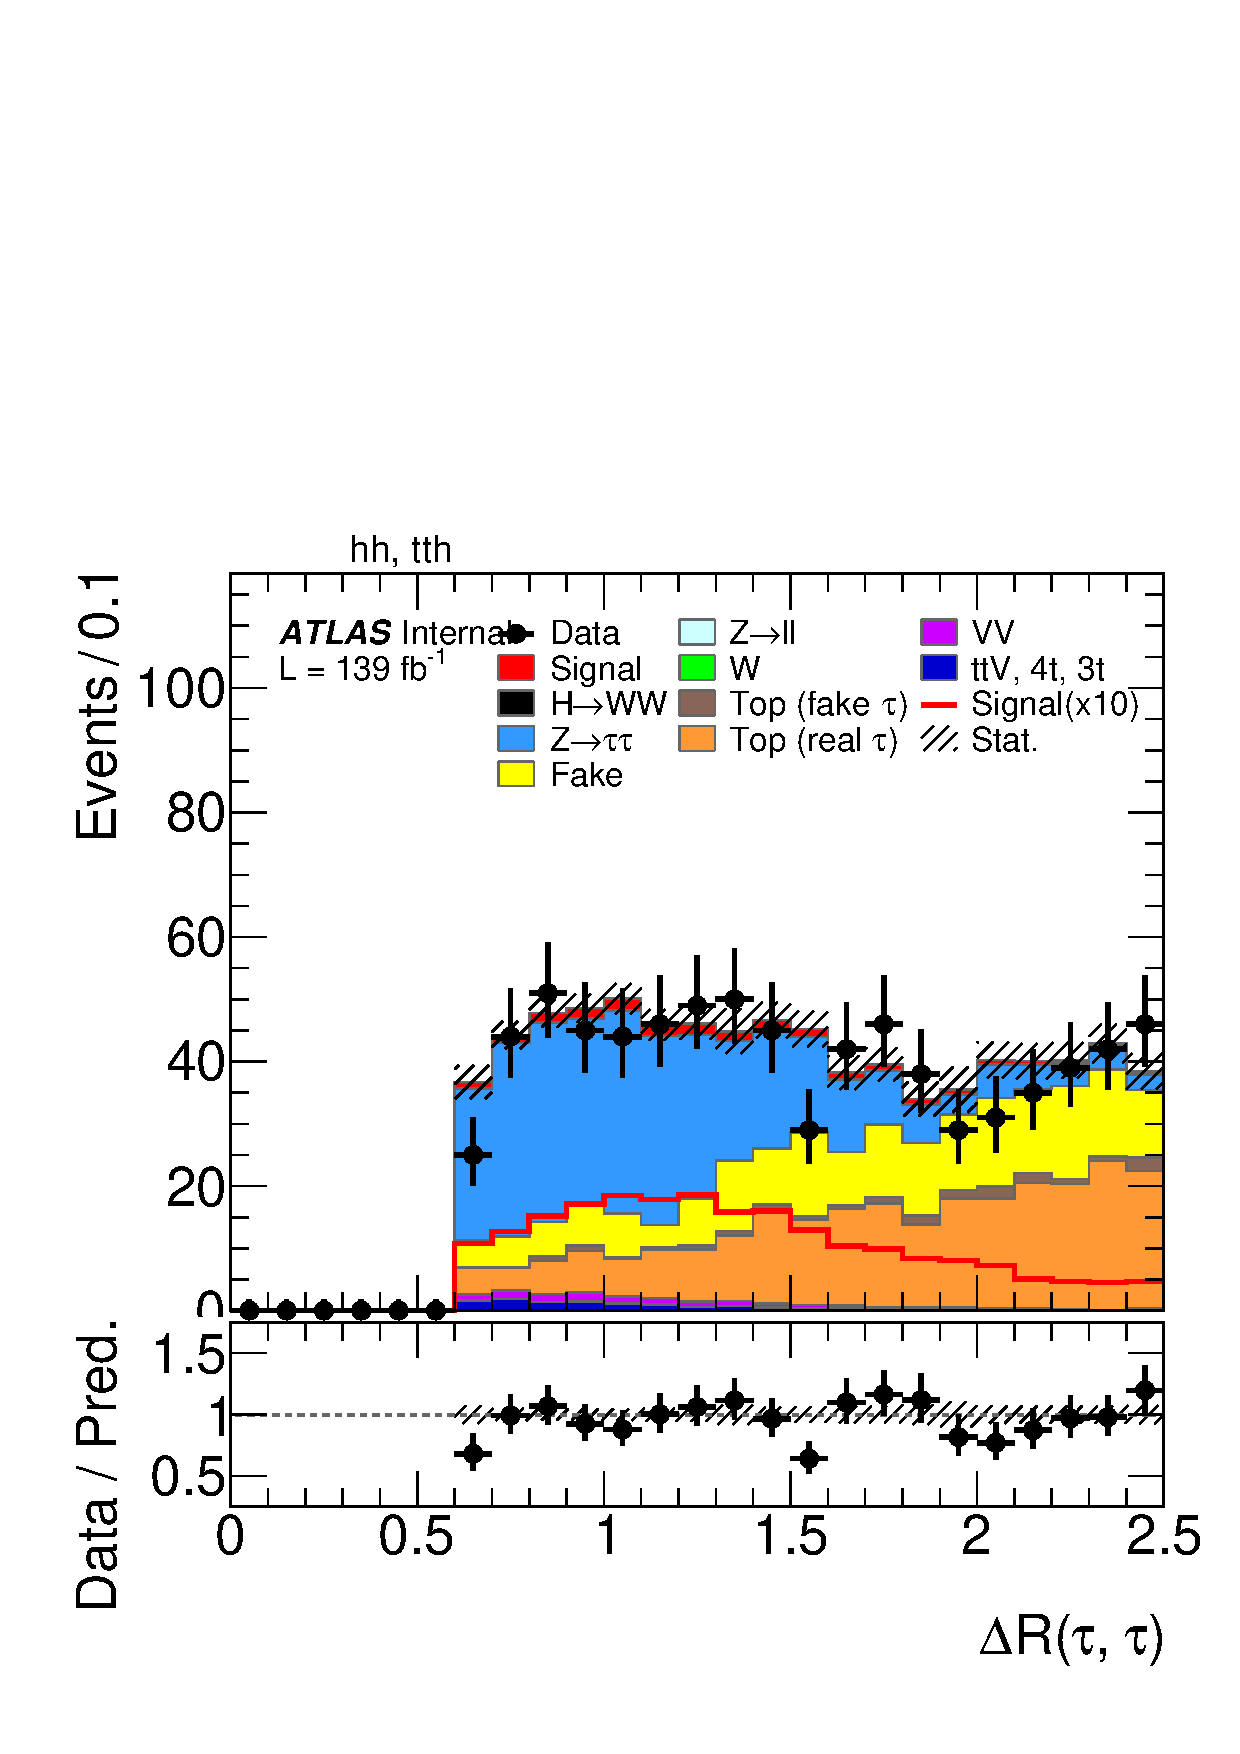
\includegraphics[width=0.33\textwidth]{images/modelling_tmva_vars/plot_ditau_dr_hh_tth.pdf} &
      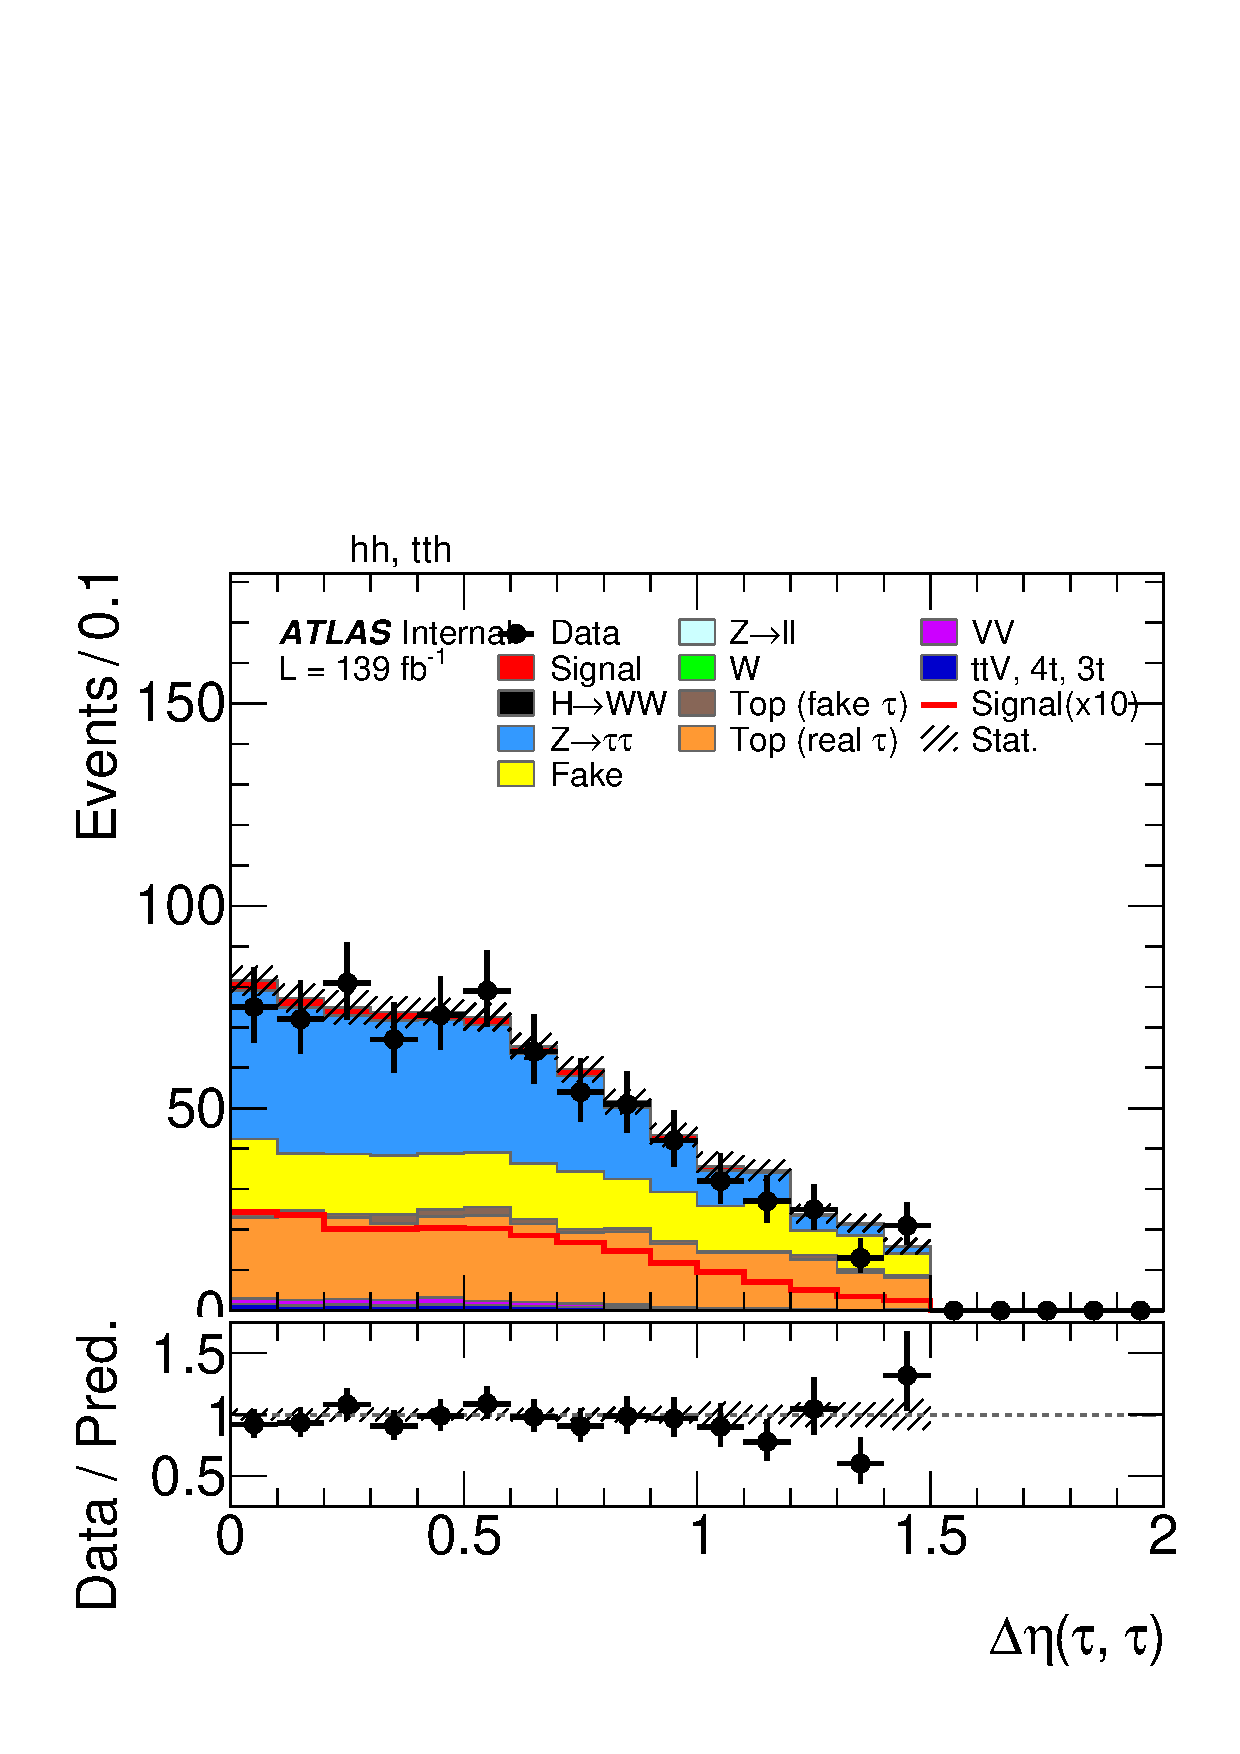
\includegraphics[width=0.33\textwidth]{images/modelling_tmva_vars/plot_ditau_deta_hh_tth.pdf} &
      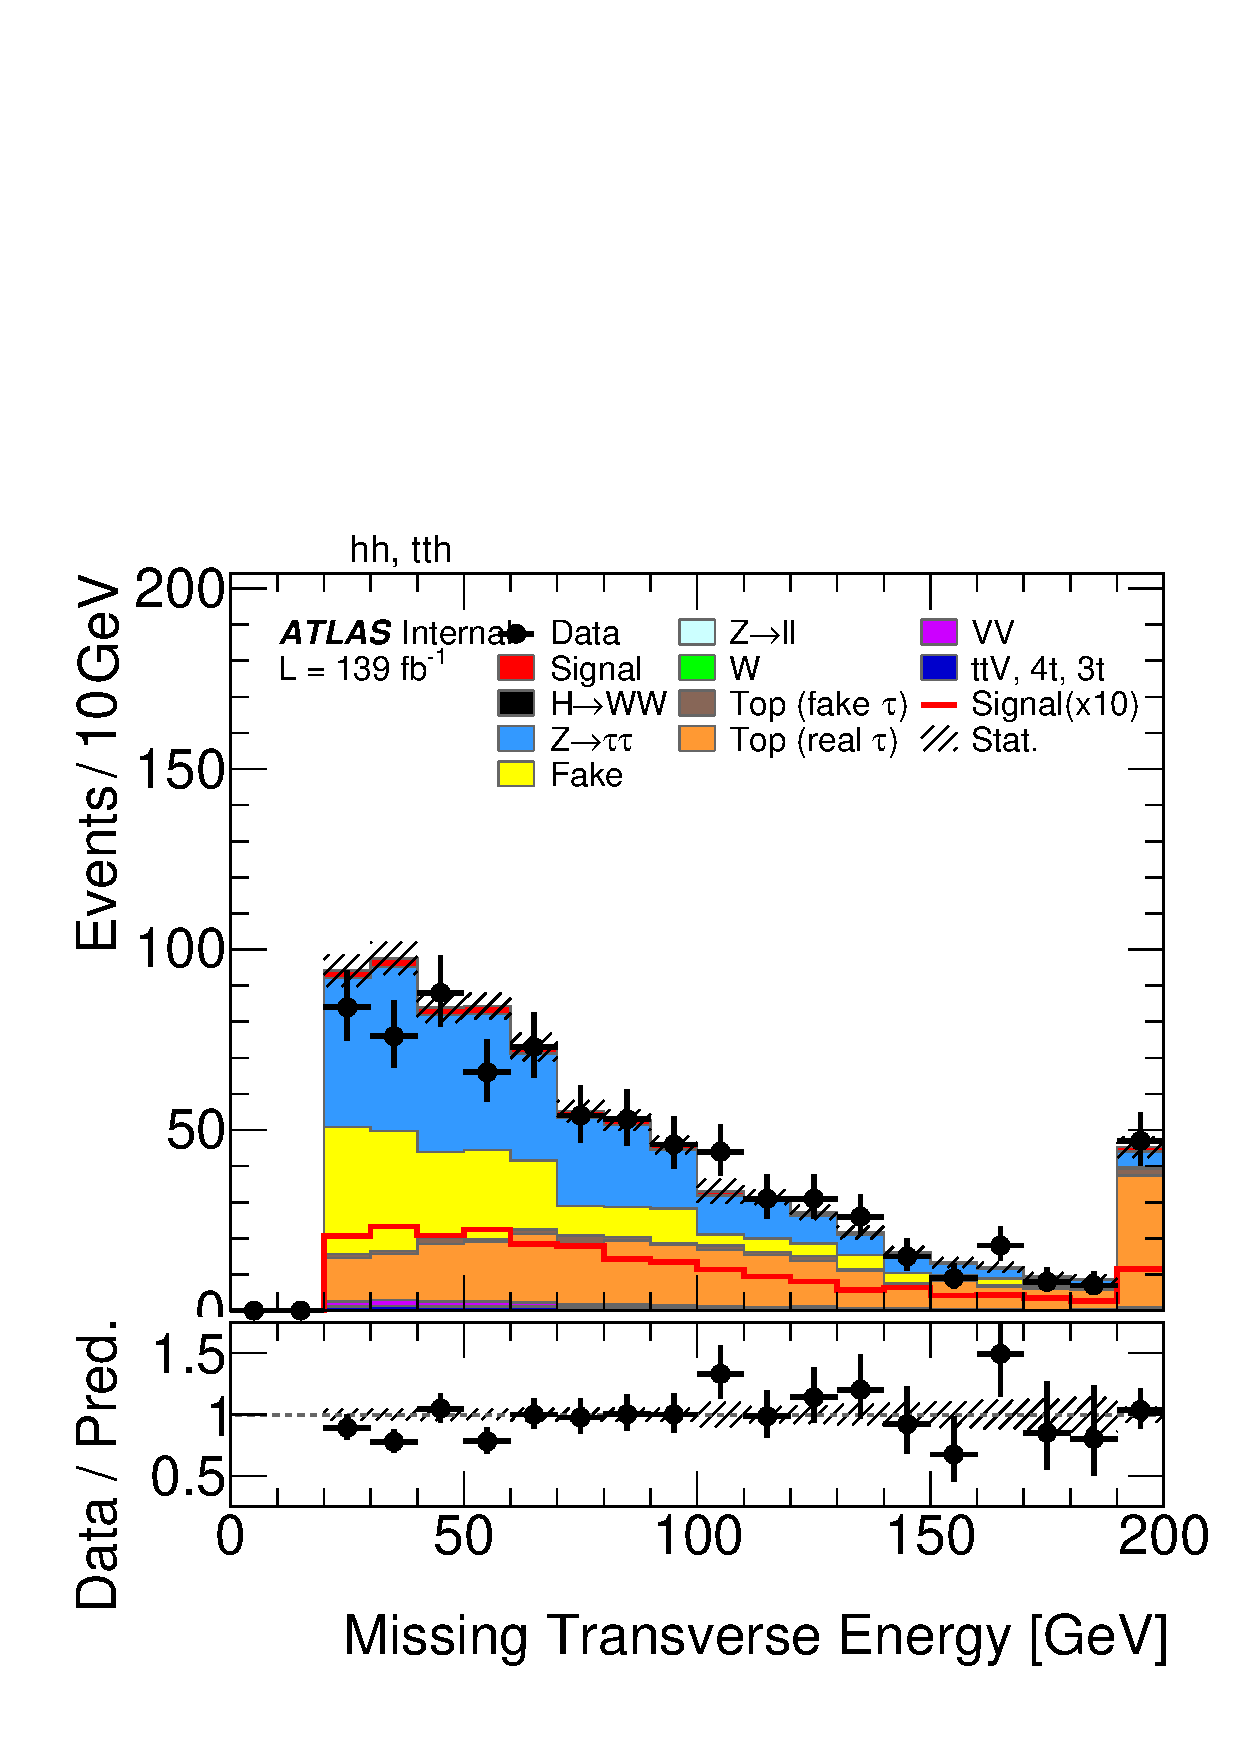
\includegraphics[width=0.33\textwidth]{images/modelling_tmva_vars/plot_met_reco_et_hh_tth.pdf} \\[4pt]
      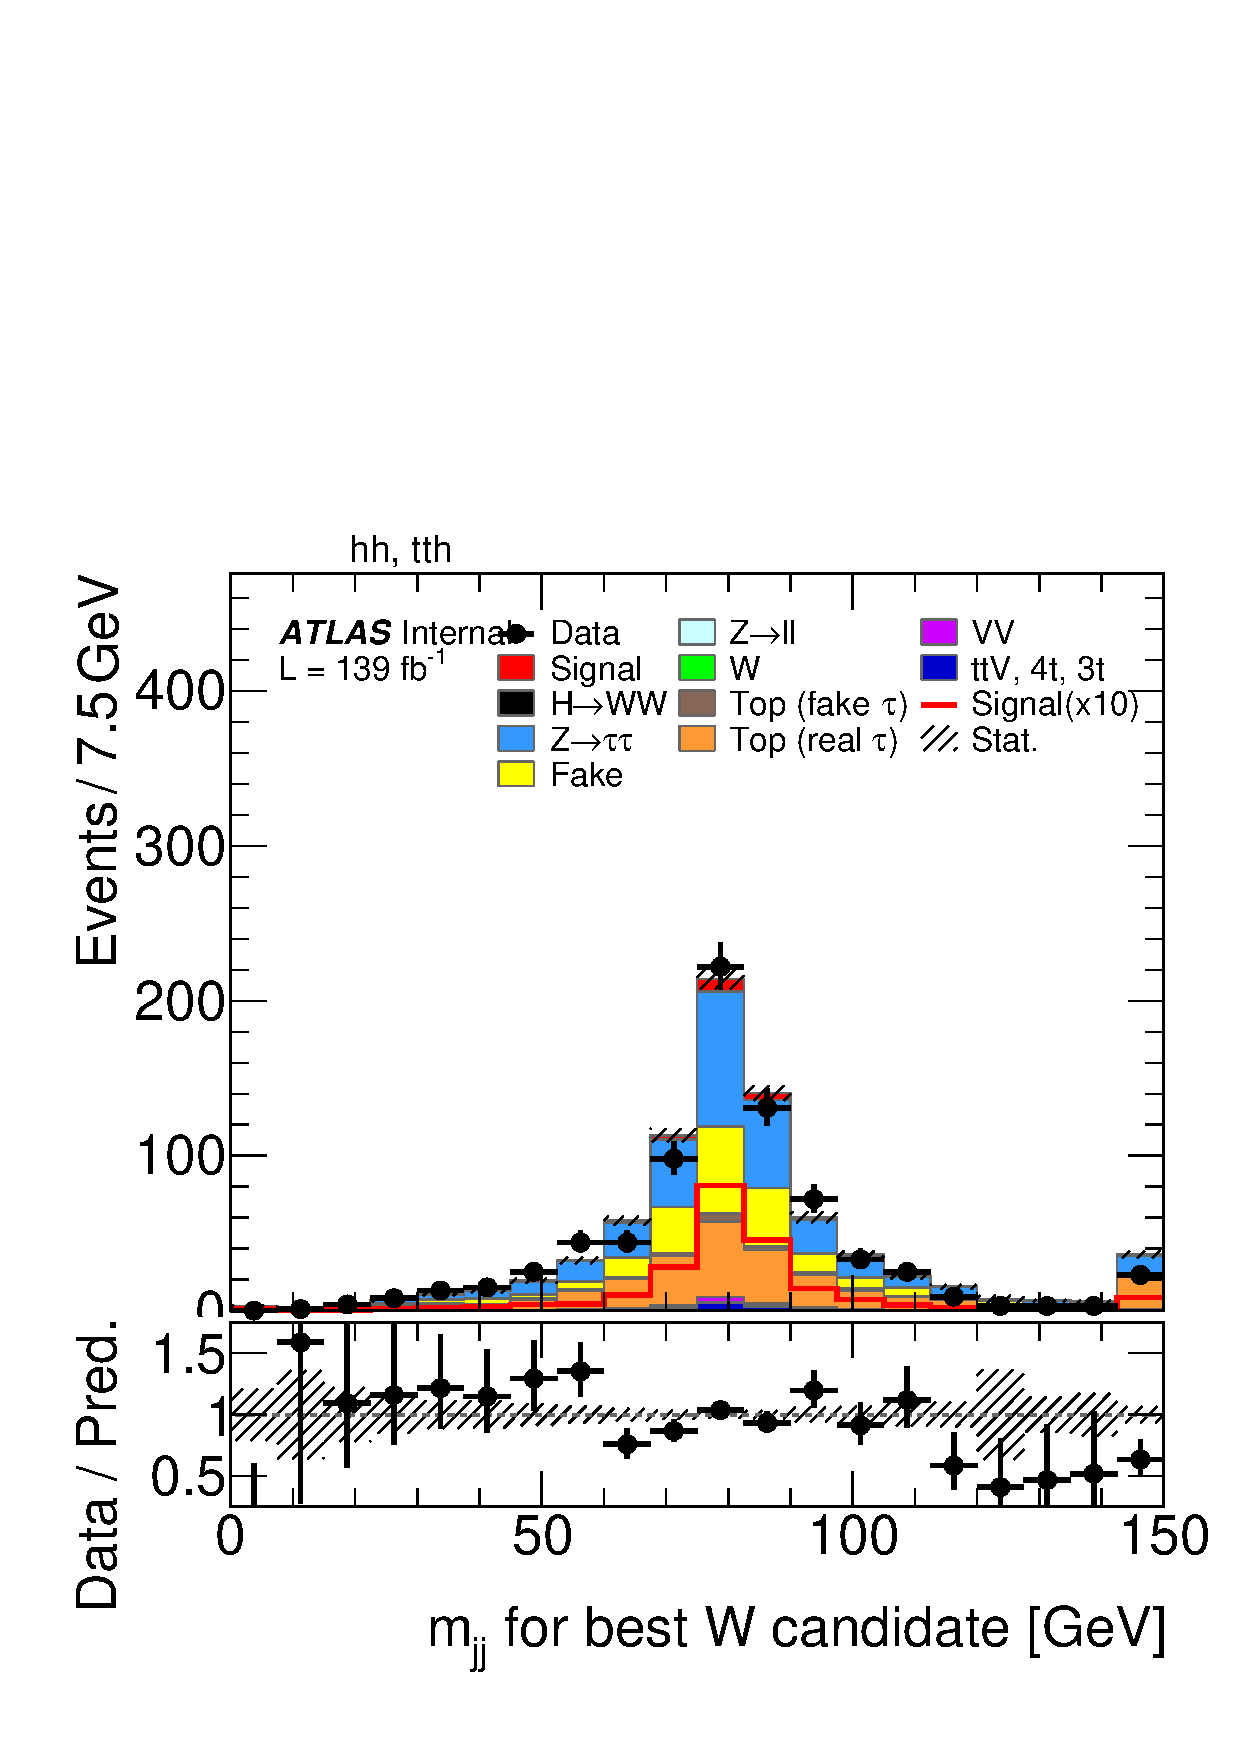
\includegraphics[width=0.33\textwidth]{images/modelling_tmva_vars/plot_mWbest_hh_tth.pdf} &
      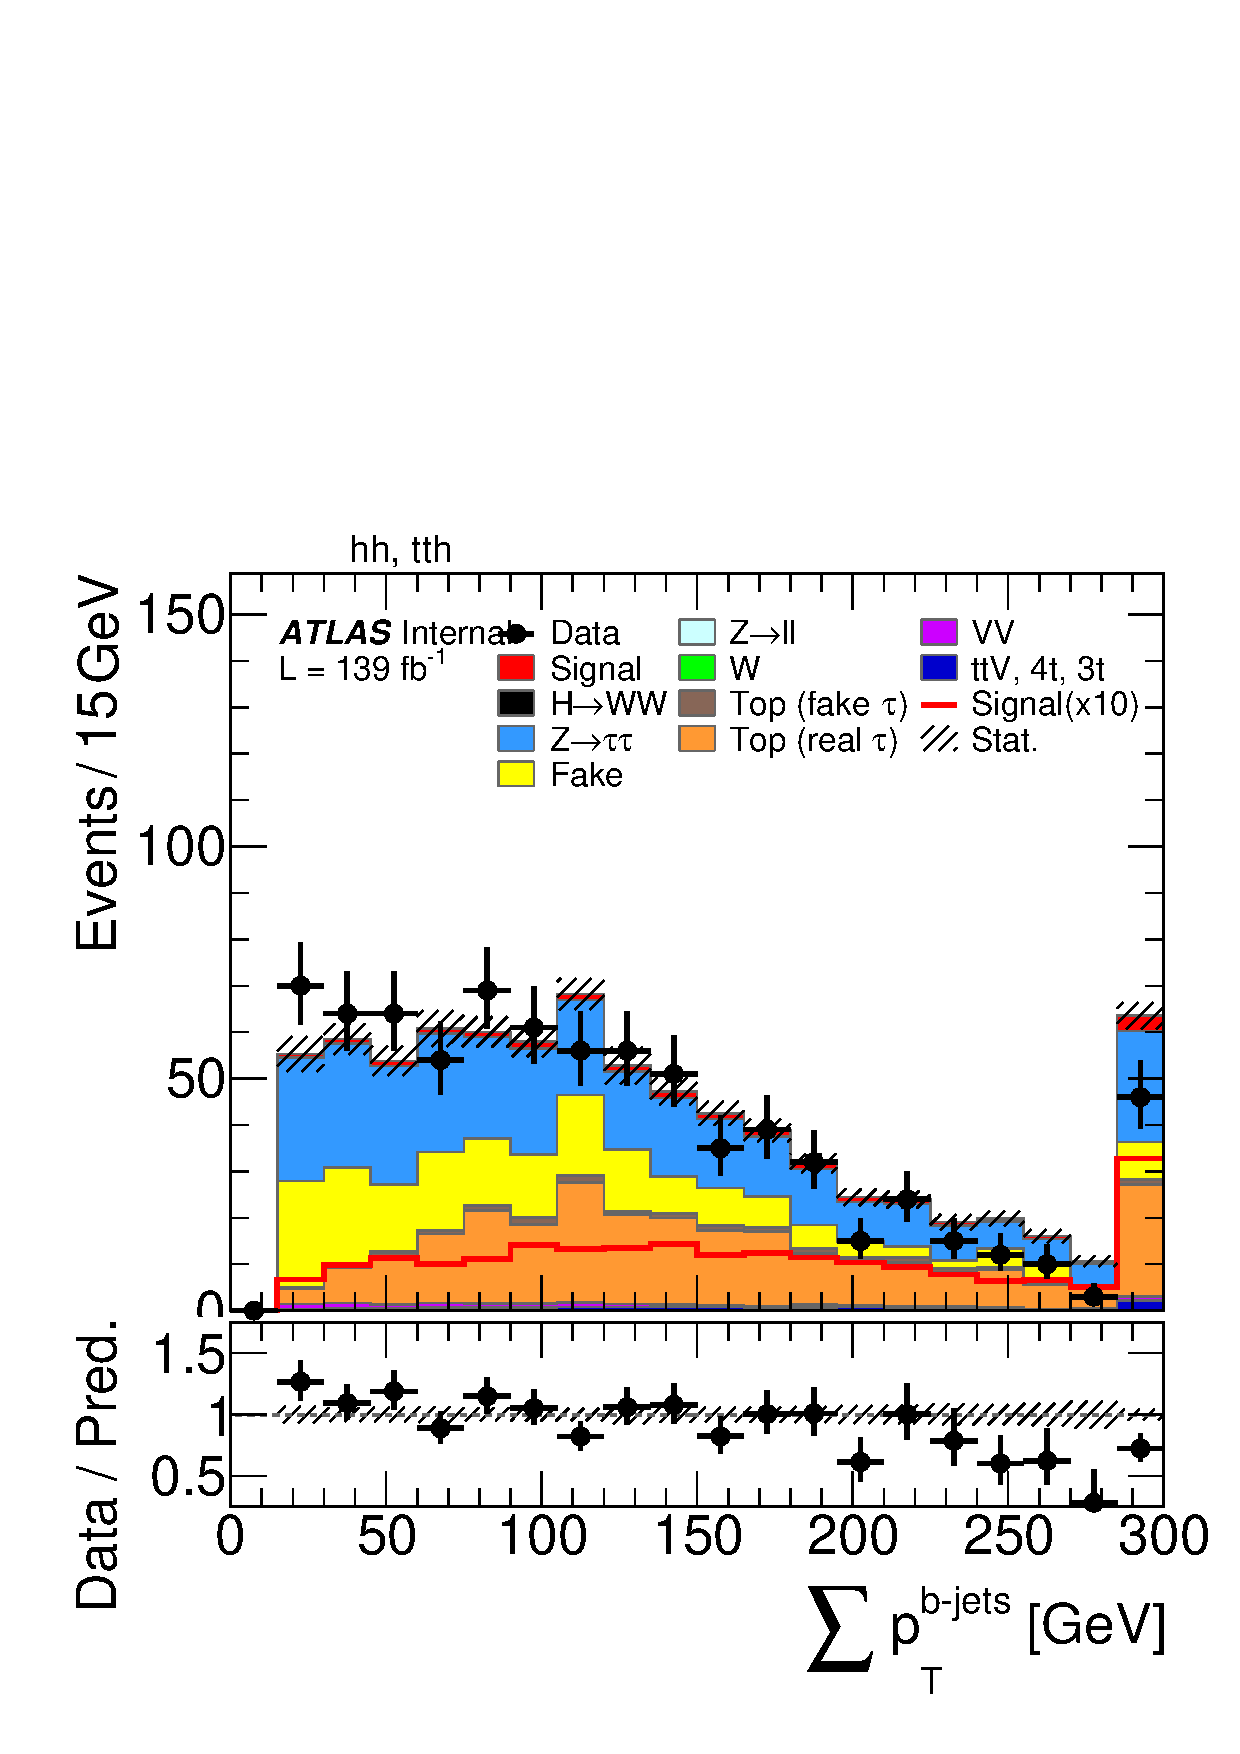
\includegraphics[width=0.33\textwidth]{images/modelling_tmva_vars/plot_SumPtBjet_hh_tth.pdf} &
      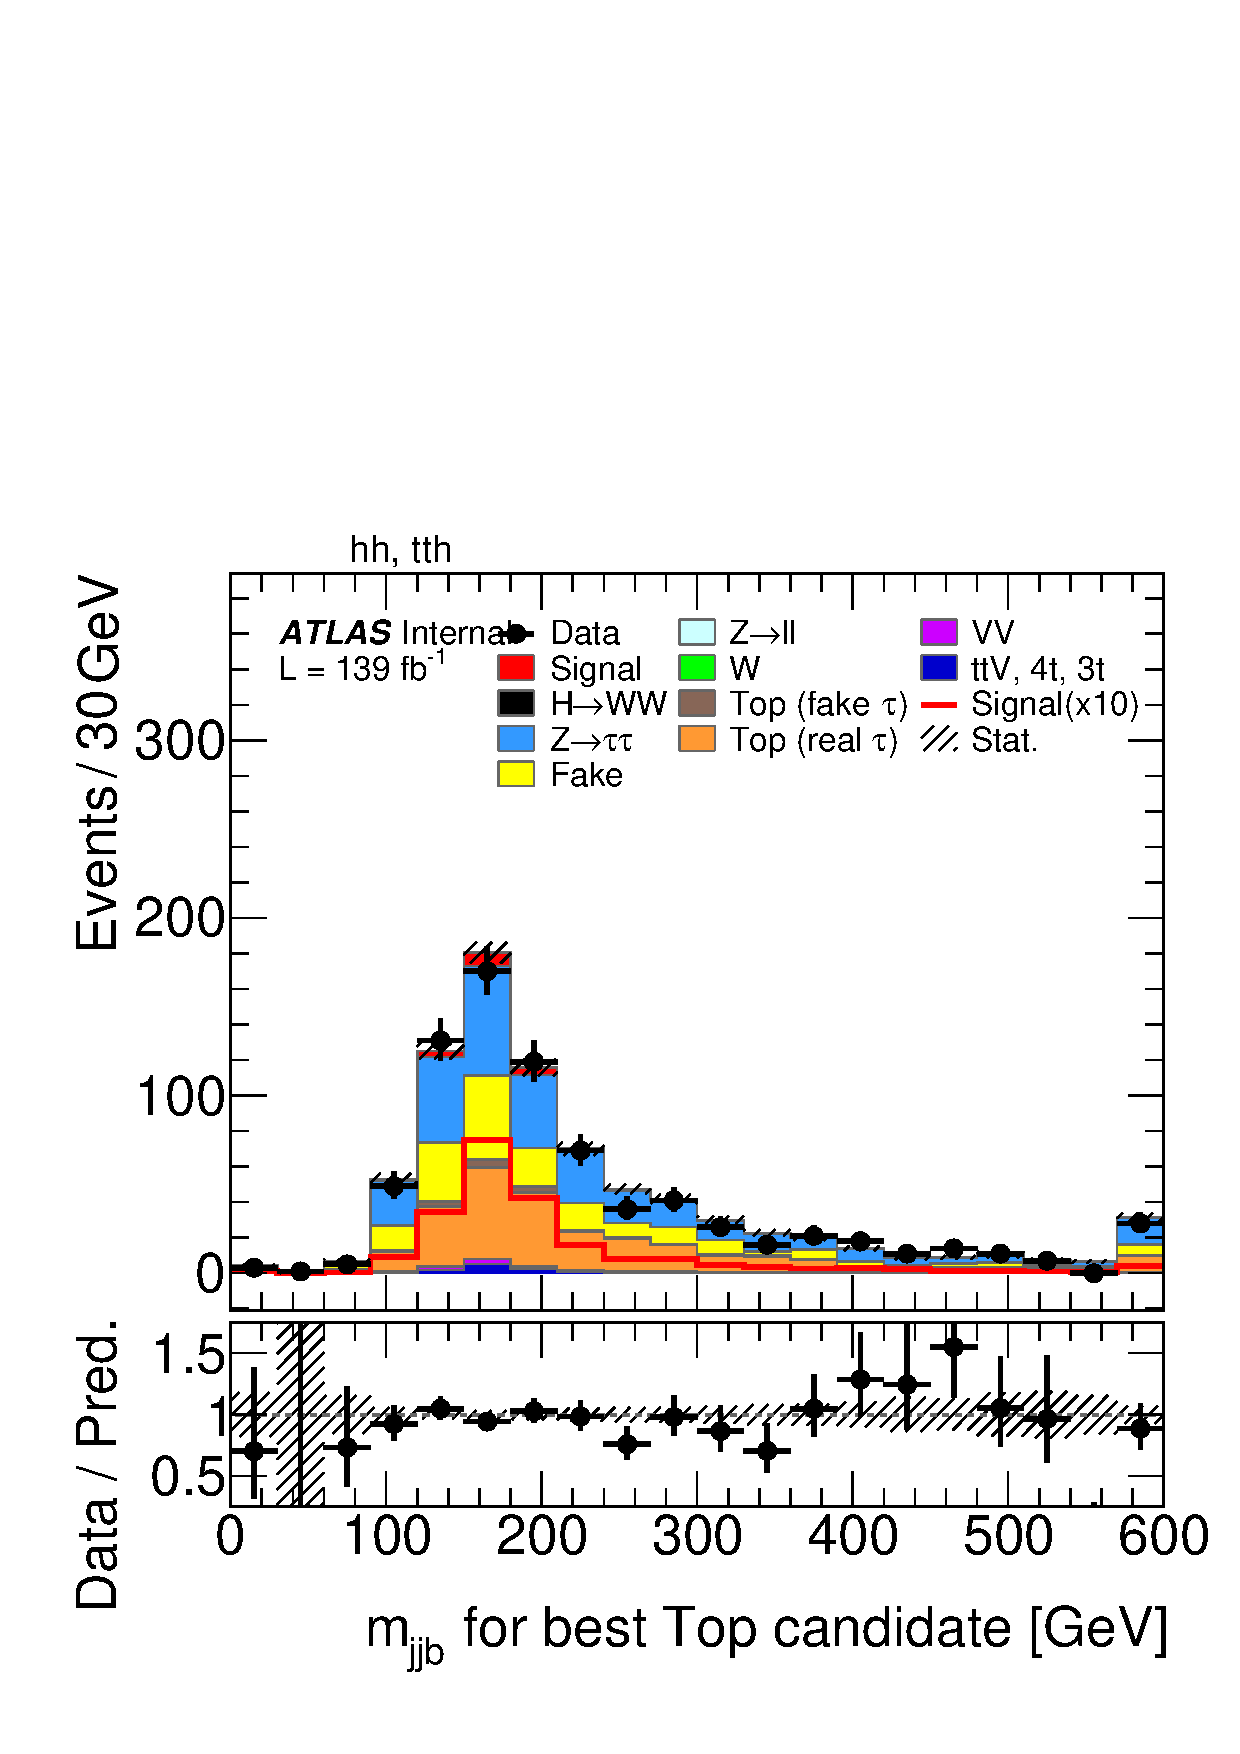
\includegraphics[width=0.33\textwidth]{images/modelling_tmva_vars/plot_mTopWbest_hh_tth.pdf} \\[4pt]
      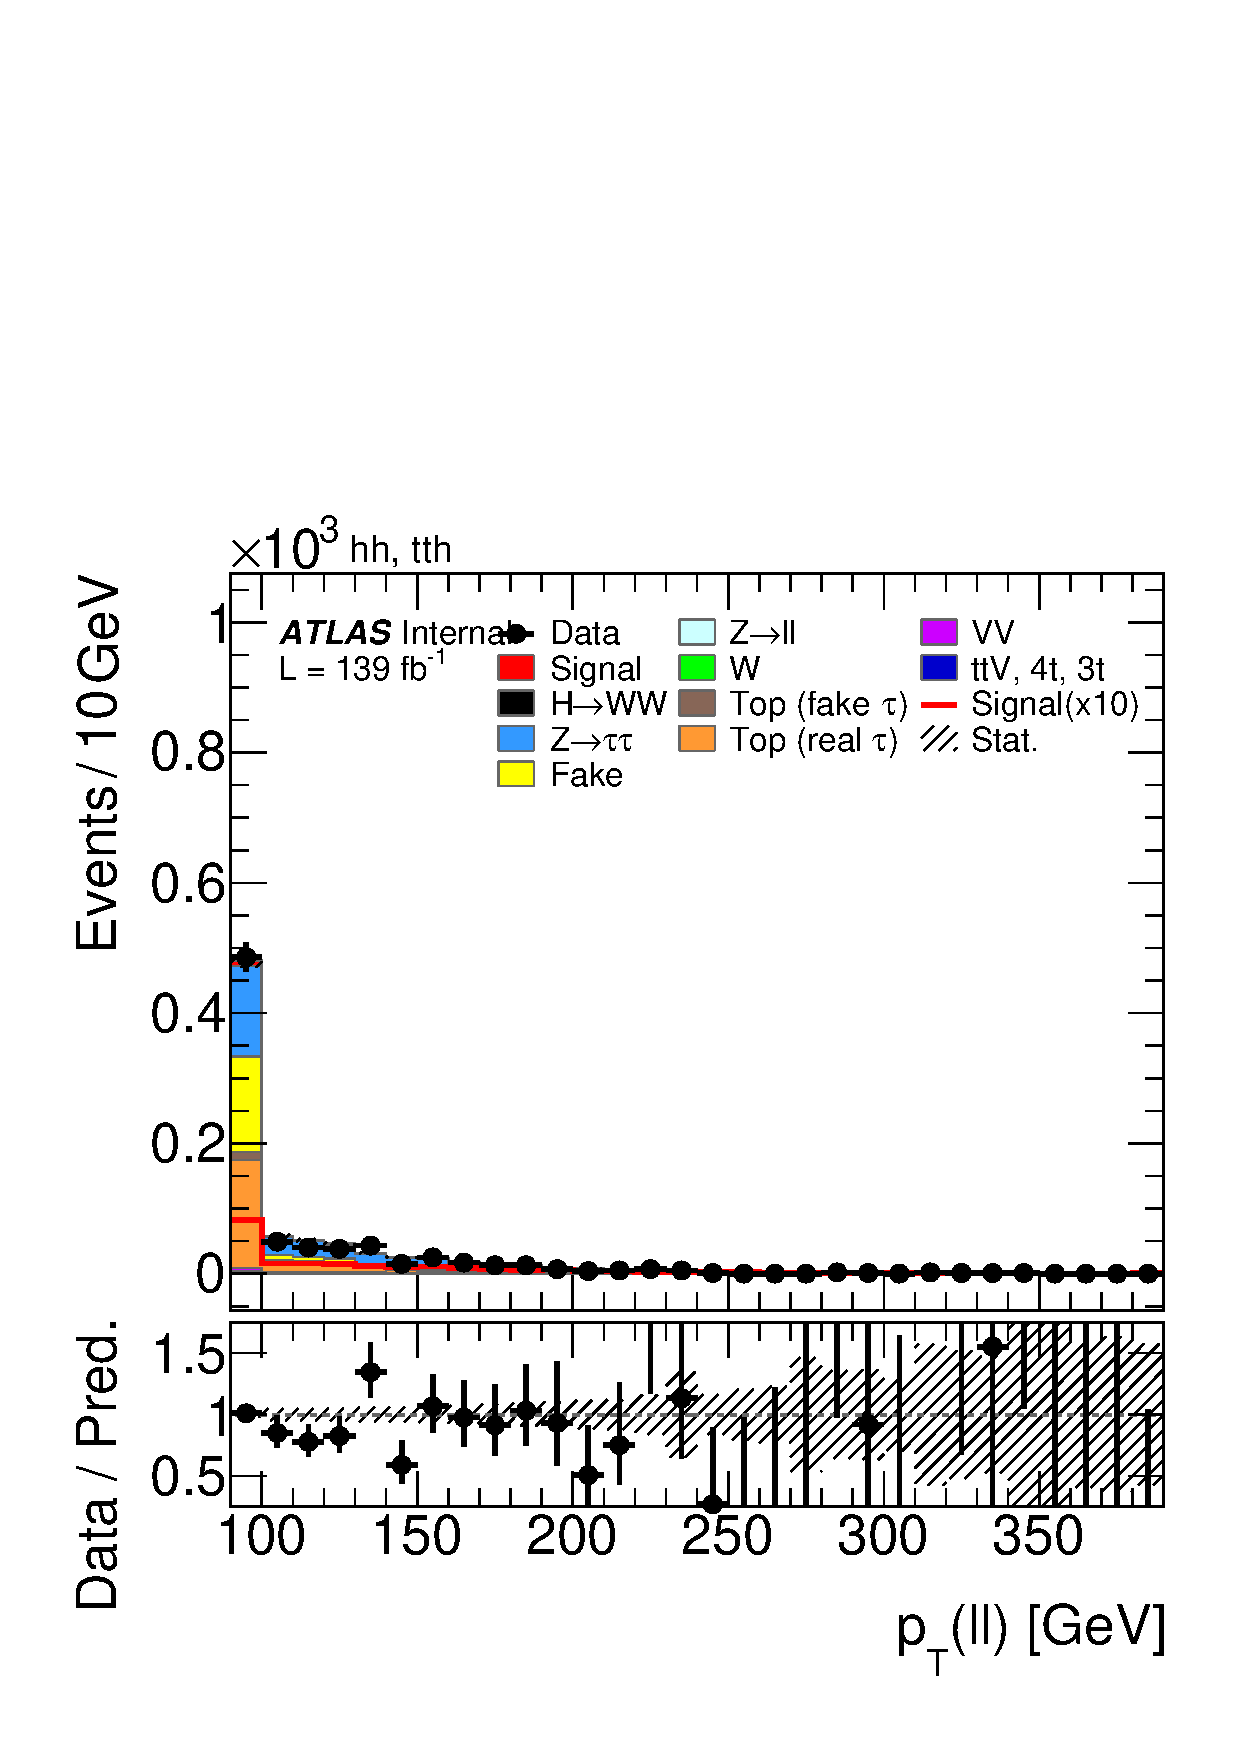
\includegraphics[width=0.33\textwidth]{images/modelling_tmva_vars/plot_ditau_pt_hh_tth.pdf} &
      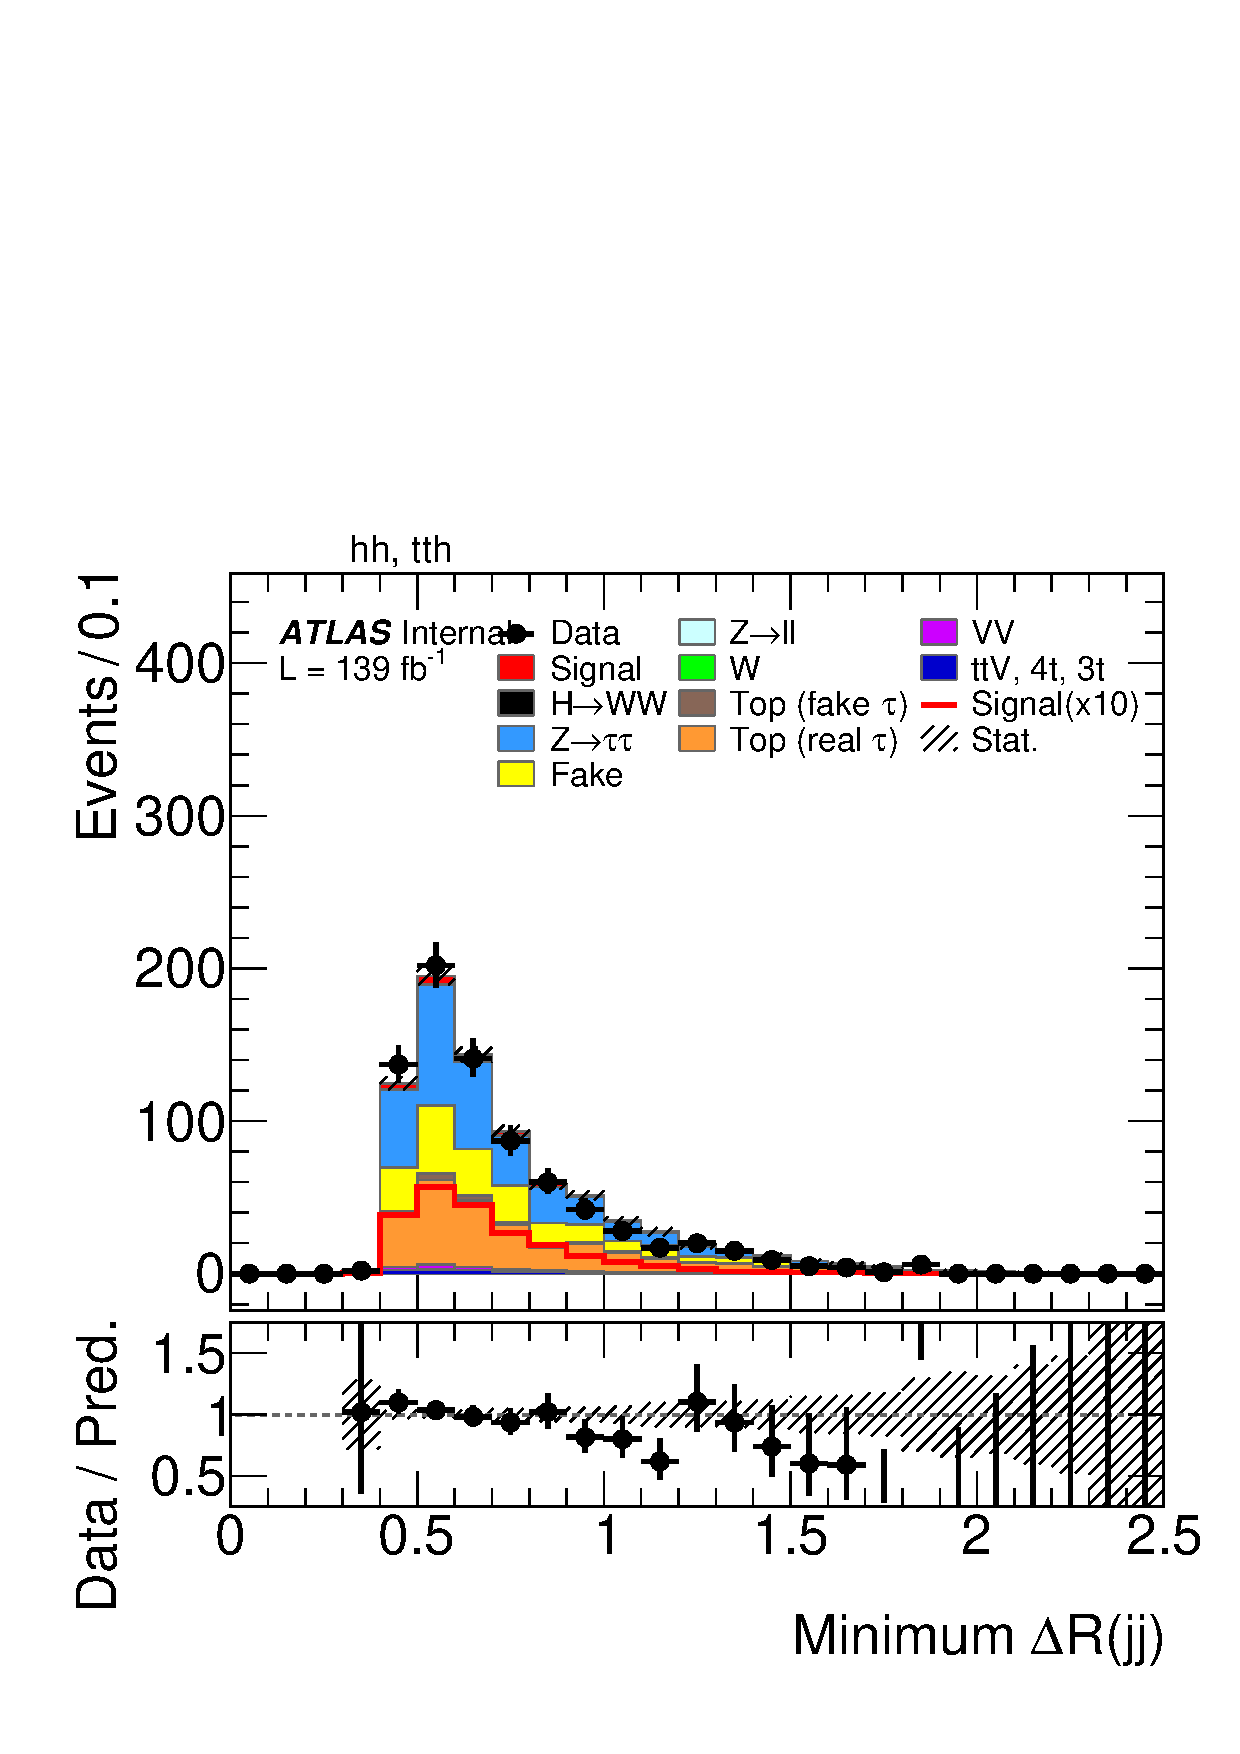
\includegraphics[width=0.33\textwidth]{images/modelling_tmva_vars/plot_jjdrmin_hh_tth.pdf} &
      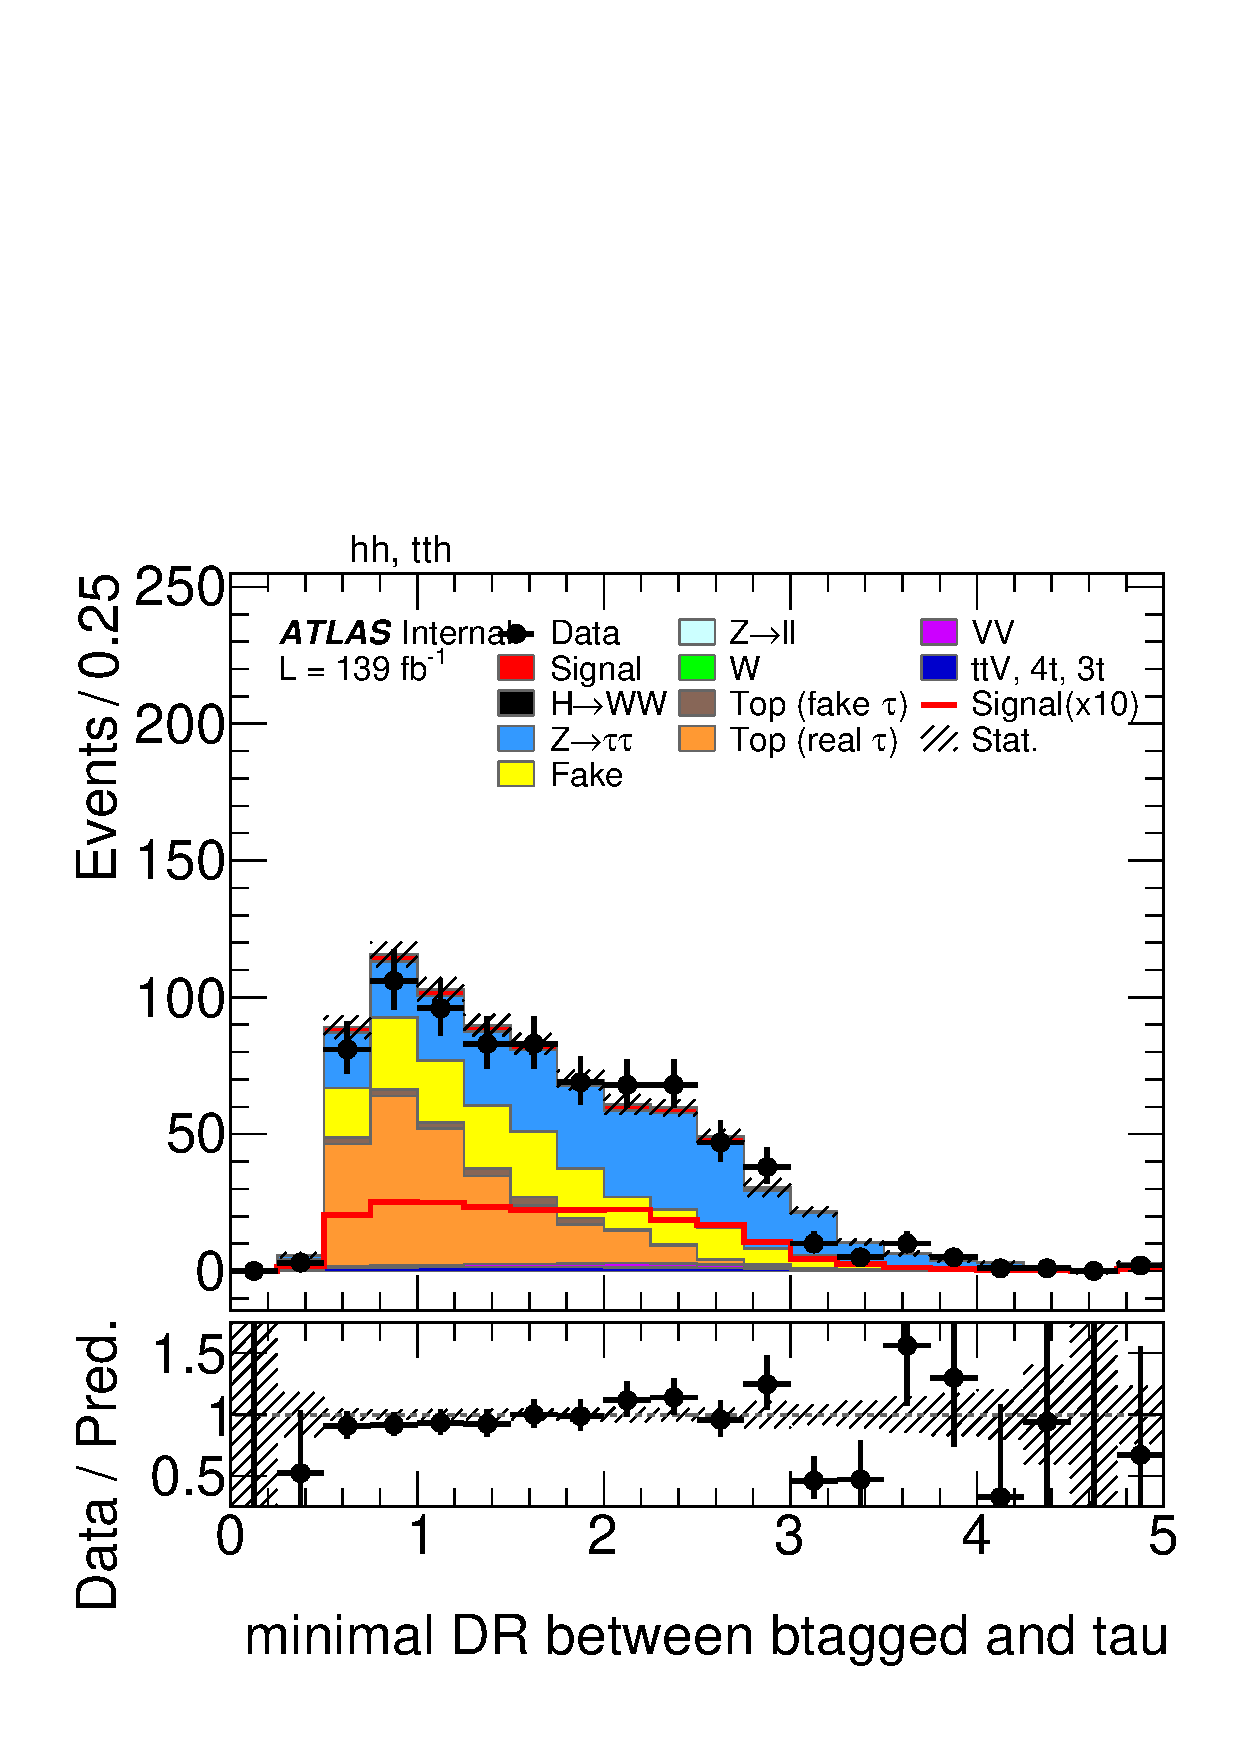
\includegraphics[width=0.33\textwidth]{images/modelling_tmva_vars/plot_minDRbtau_hh_tth.pdf}
    \end{tabular}
  
    \caption{Data/MC modelling for the \ttH BDT input variables at the \ttHtt preselection. Only statistical uncertainties are shown.}
    \label{tth_vars_modelling_1}
\end{figure}

\begin{figure}[htbp]
  \centering
  \setlength{\tabcolsep}{1.5pt}
  \renewcommand{\arraystretch}{0}

  \begin{tabular}{@{}c c c@{}}
    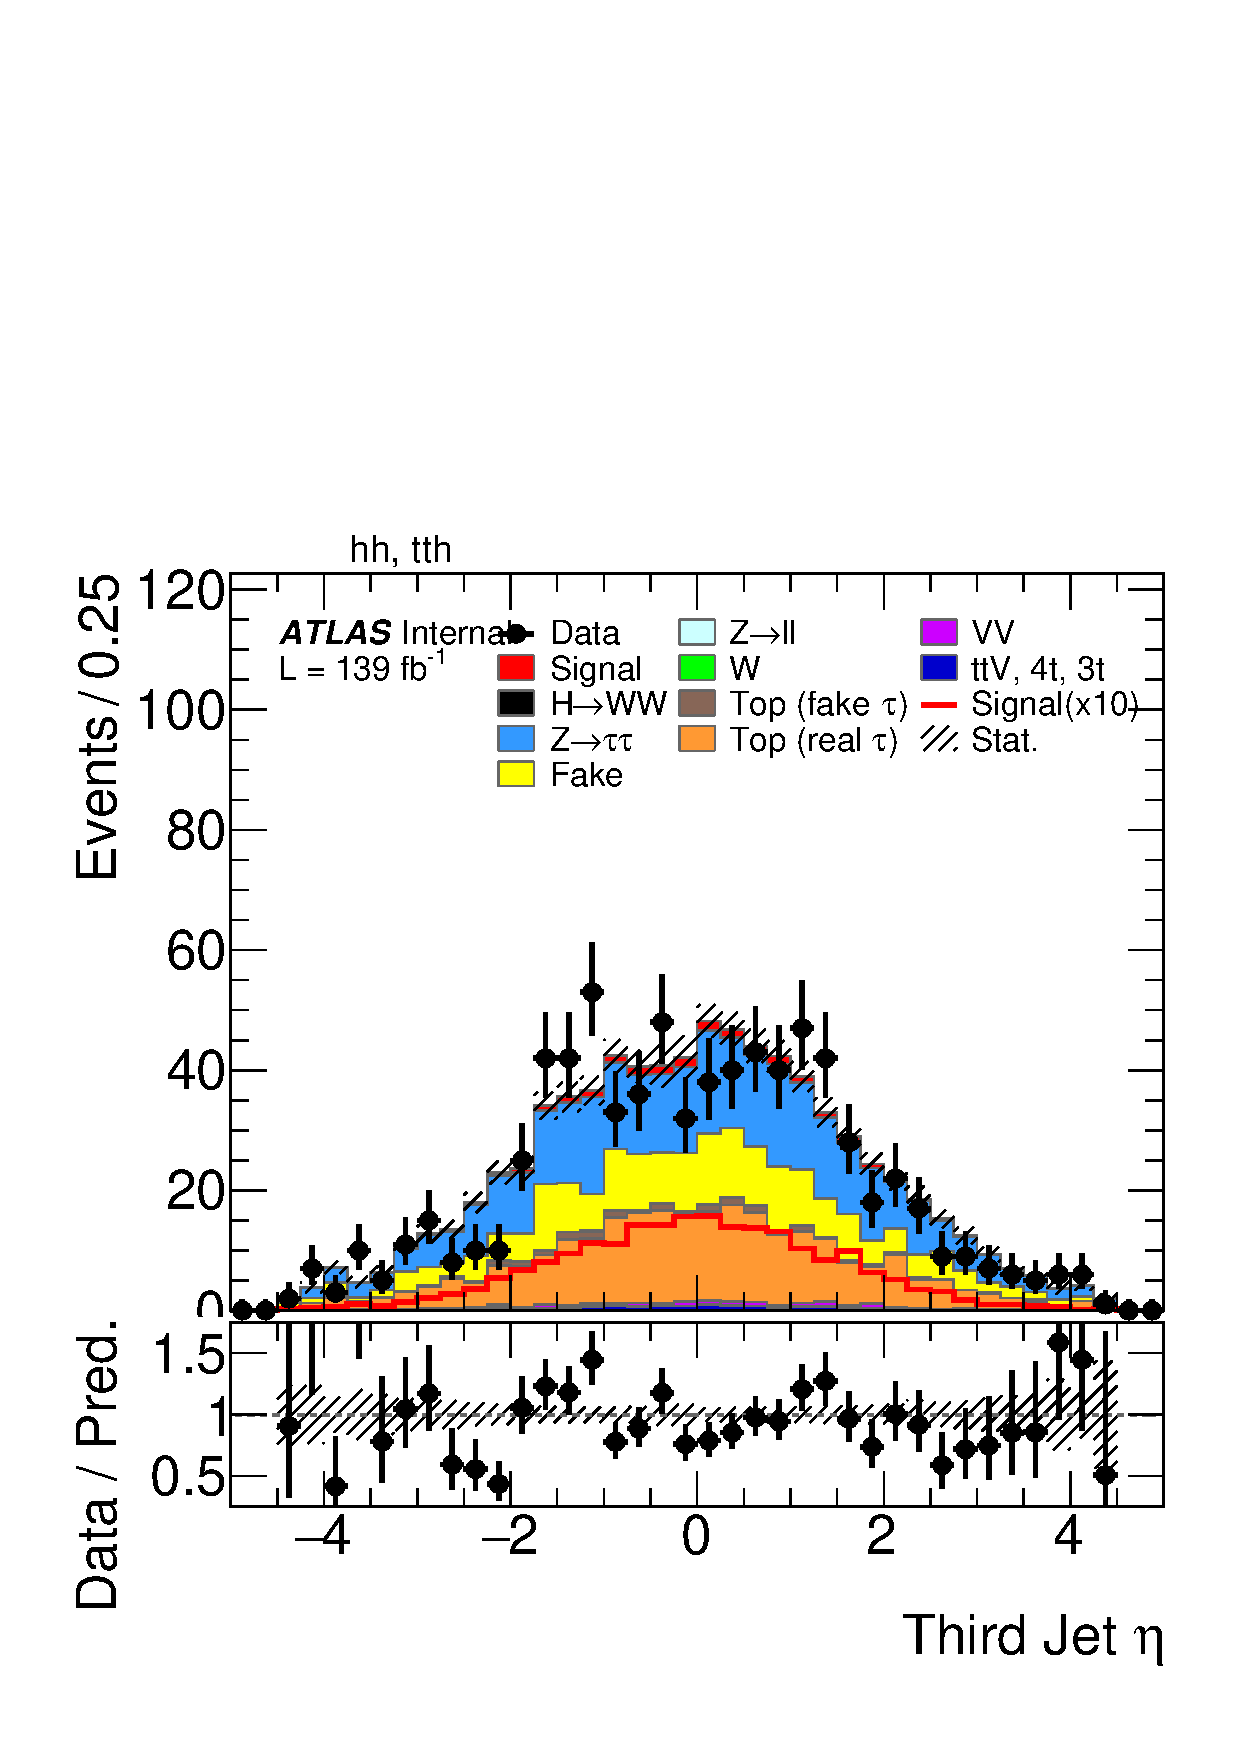
\includegraphics[width=0.33\textwidth]{images/modelling_tmva_vars/plot_jet_2_eta_hh_tth.pdf} &
    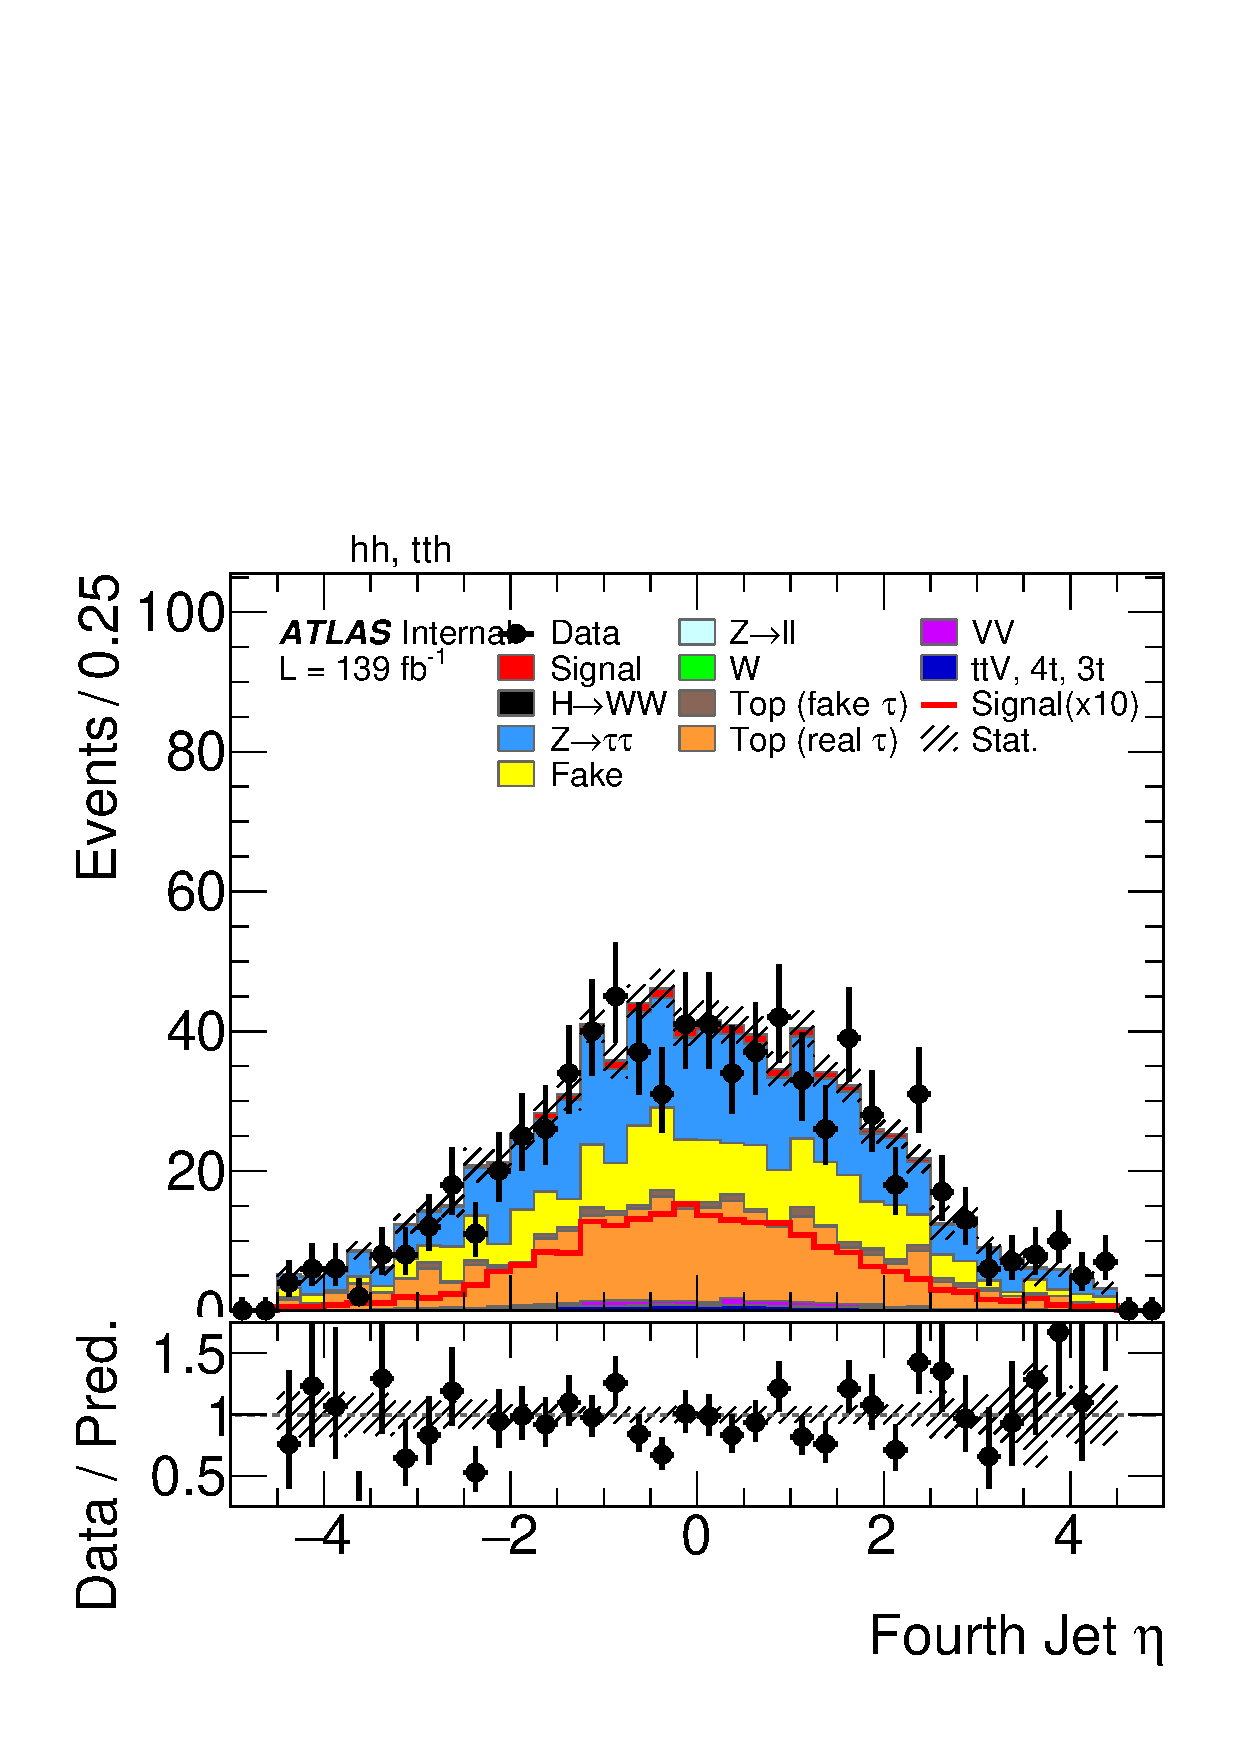
\includegraphics[width=0.33\textwidth]{images/modelling_tmva_vars/plot_jet_3_eta_hh_tth.pdf} &
    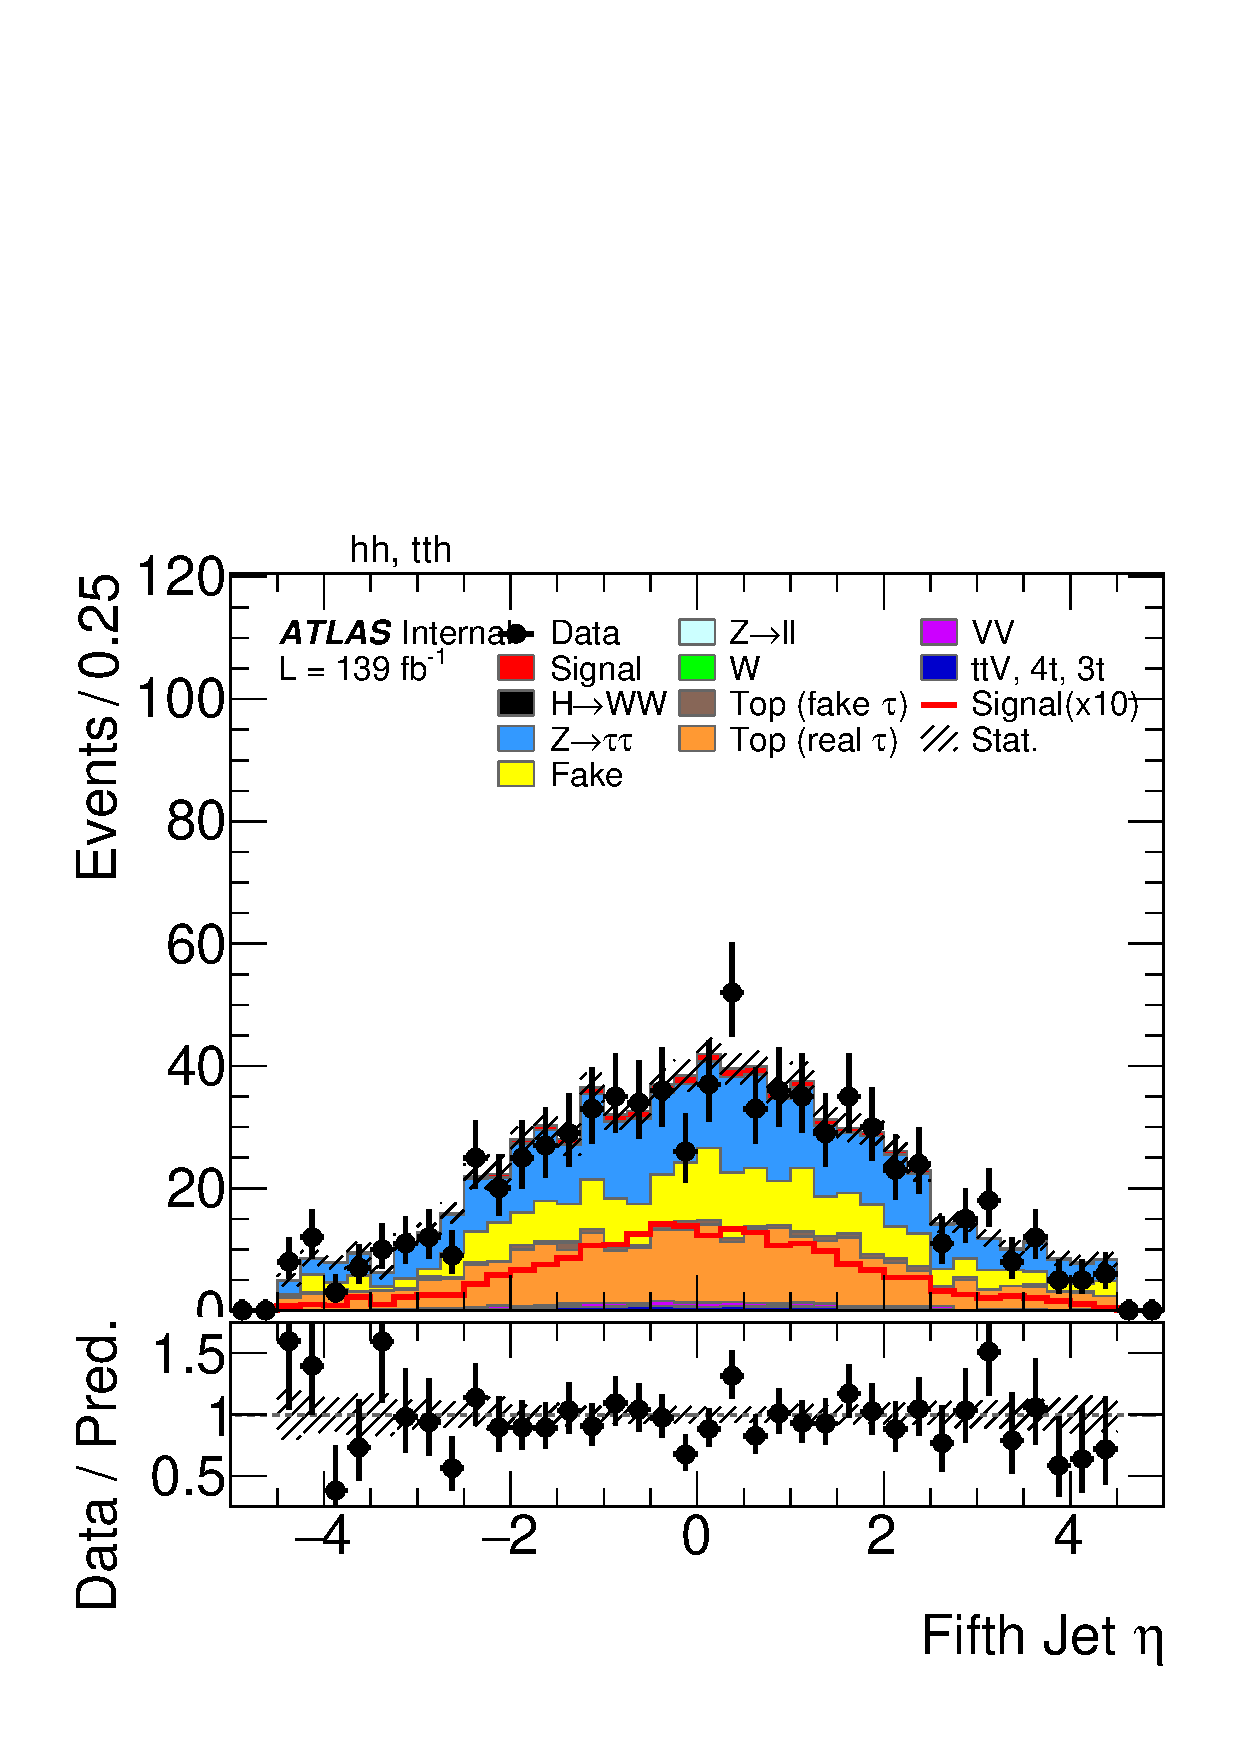
\includegraphics[width=0.33\textwidth]{images/modelling_tmva_vars/plot_jet_4_eta_hh_tth.pdf} \\[4pt]
    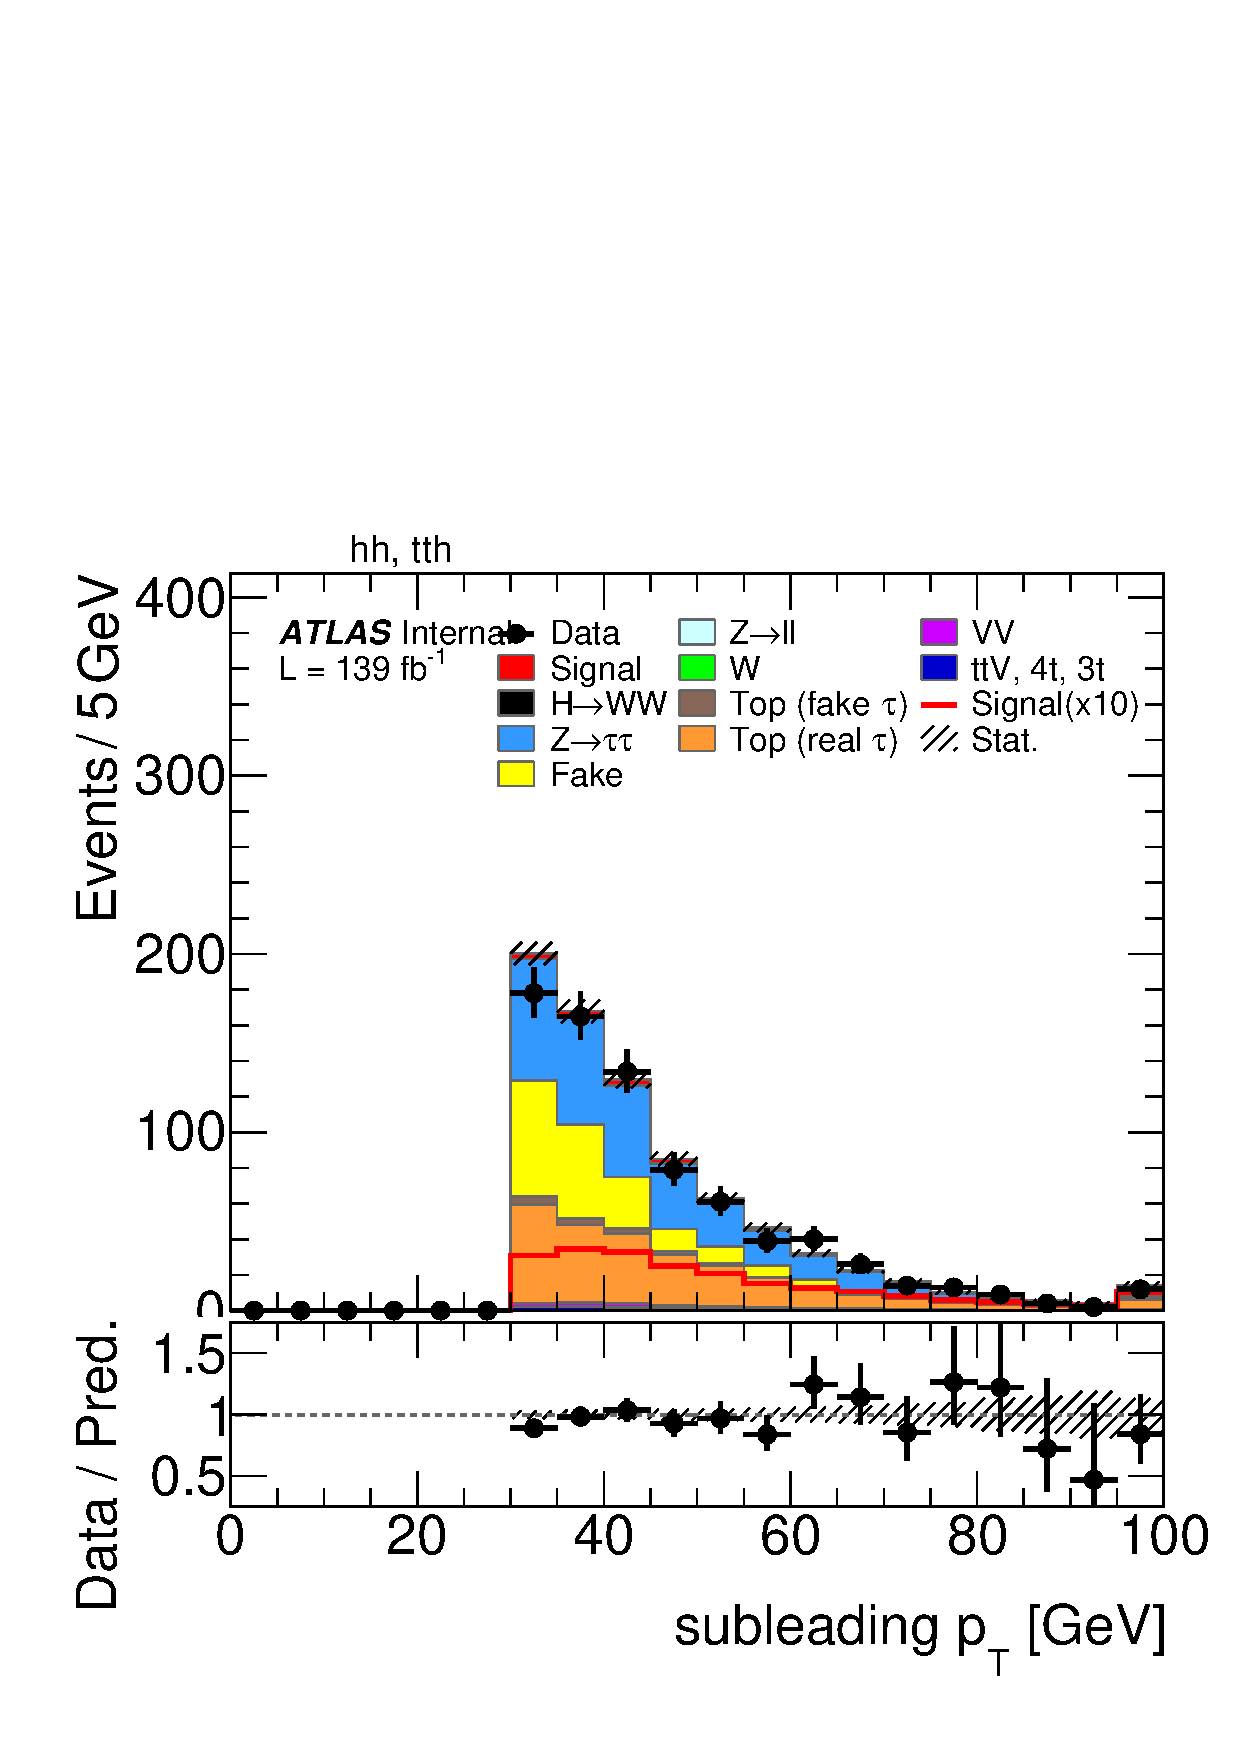
\includegraphics[width=0.33\textwidth]{images/modelling_tmva_vars/plot_tau_1_pt_hh_tth.pdf} &
    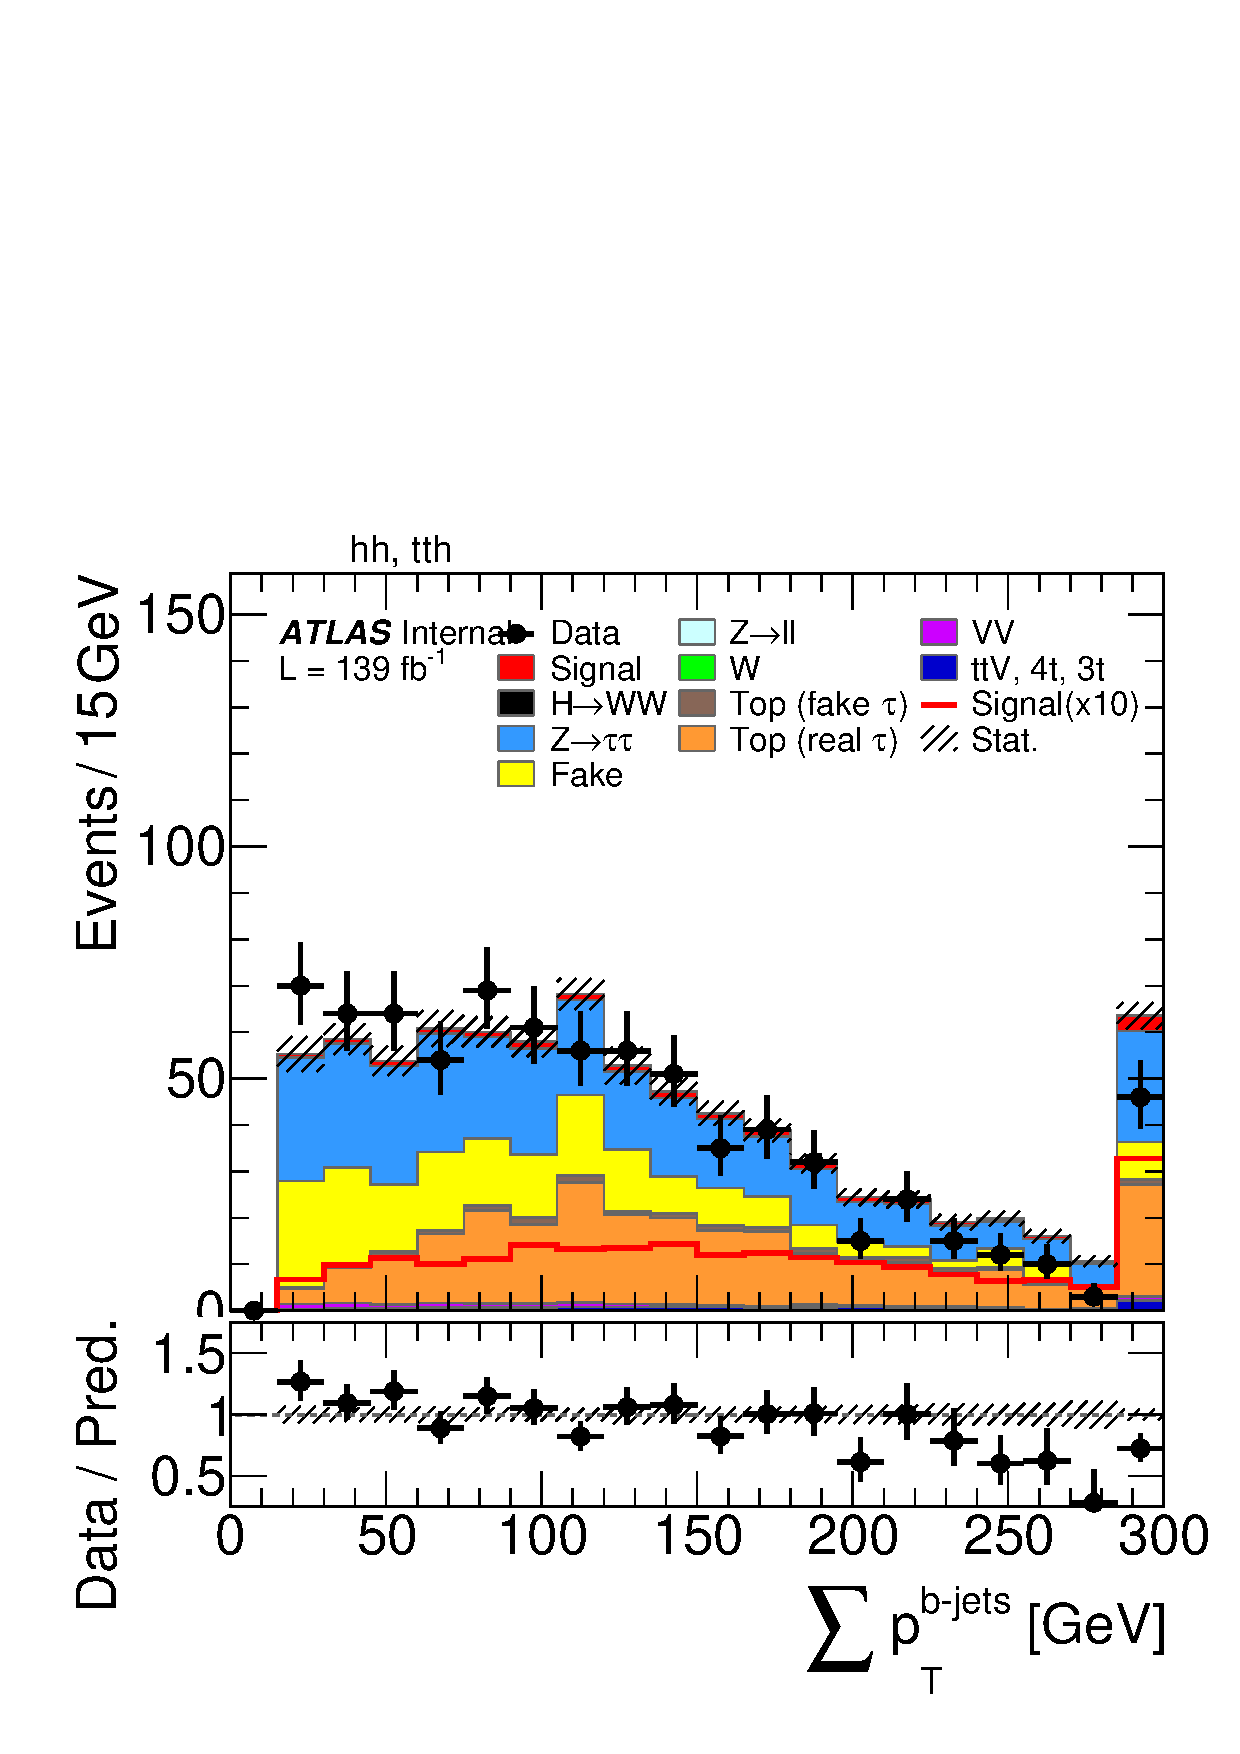
\includegraphics[width=0.33\textwidth]{images/modelling_tmva_vars/plot_SumPtBjet_hh_tth.pdf} &
    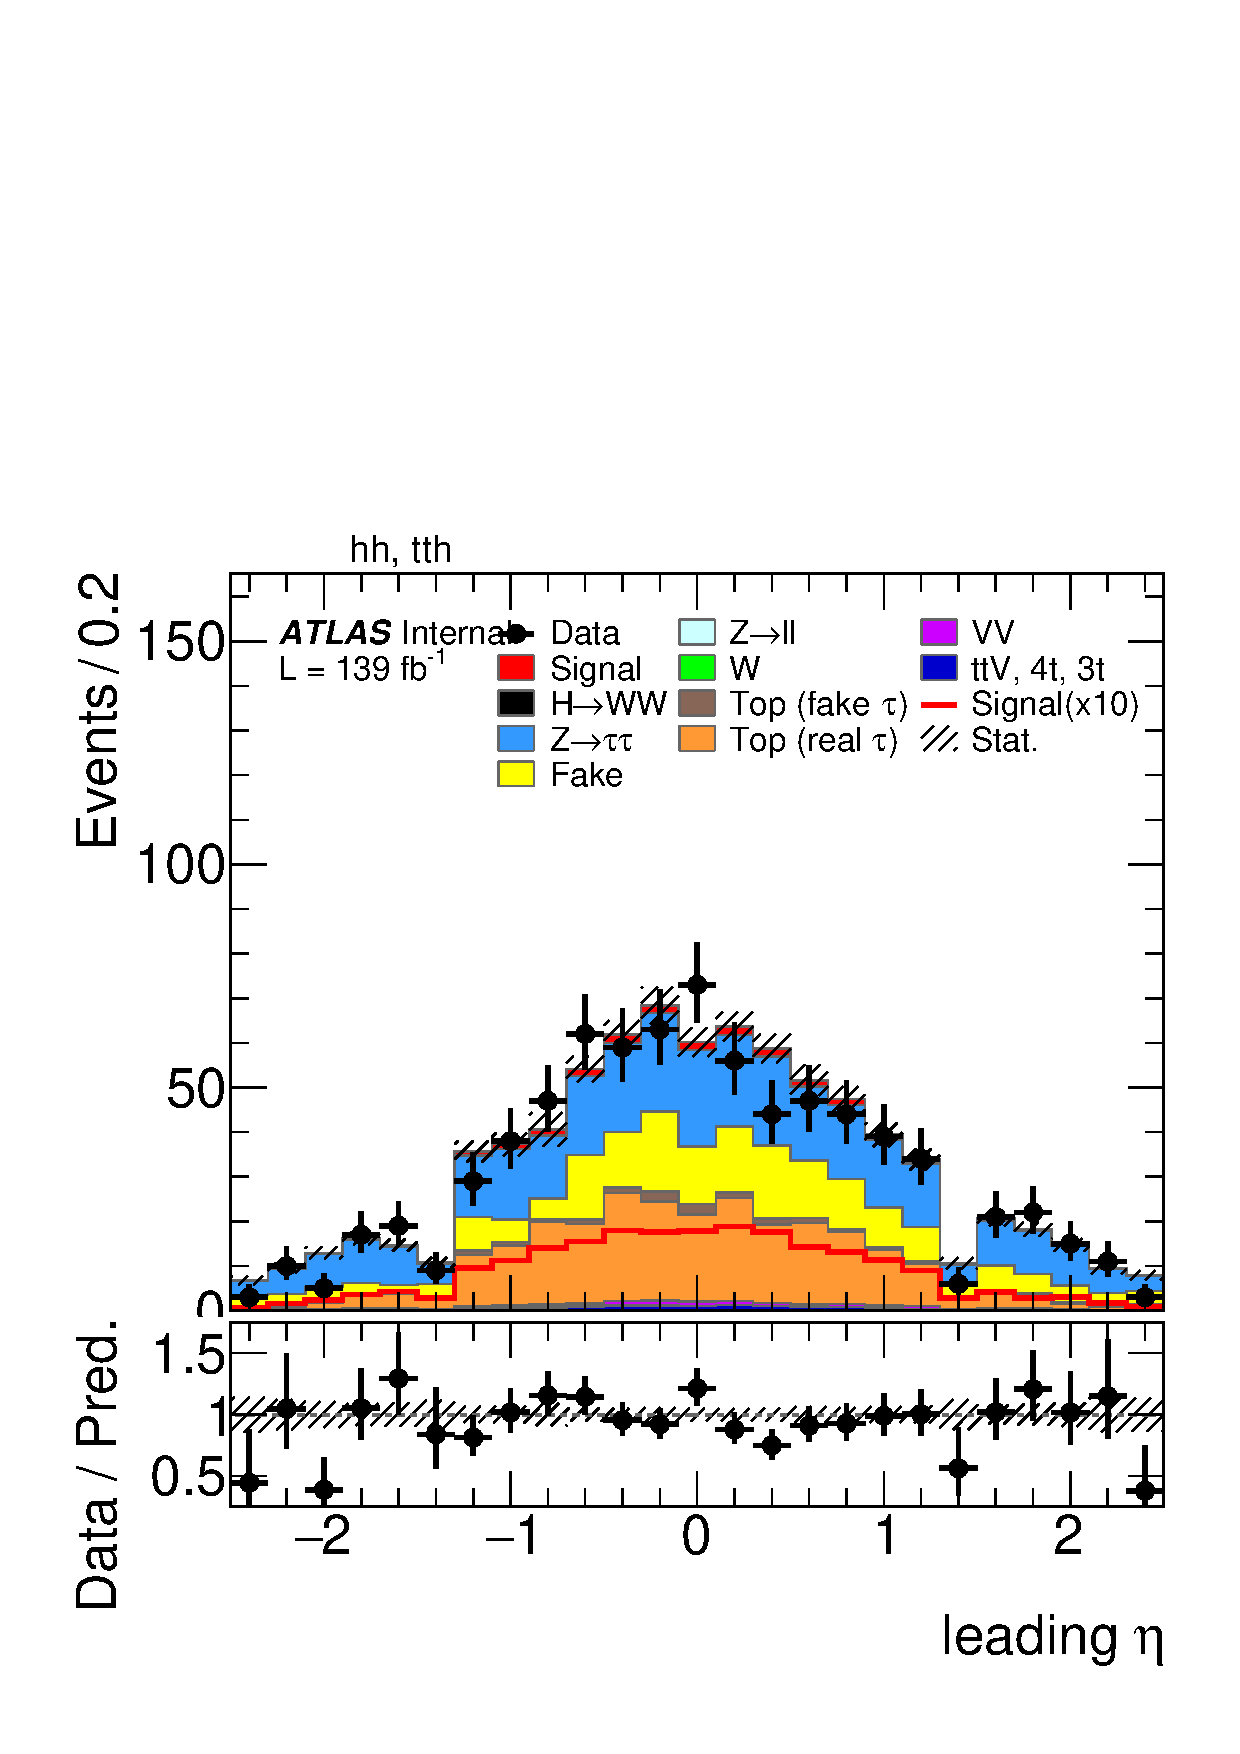
\includegraphics[width=0.33\textwidth]{images/modelling_tmva_vars/plot_tau_0_eta_hh_tth.pdf} \\[4pt]
    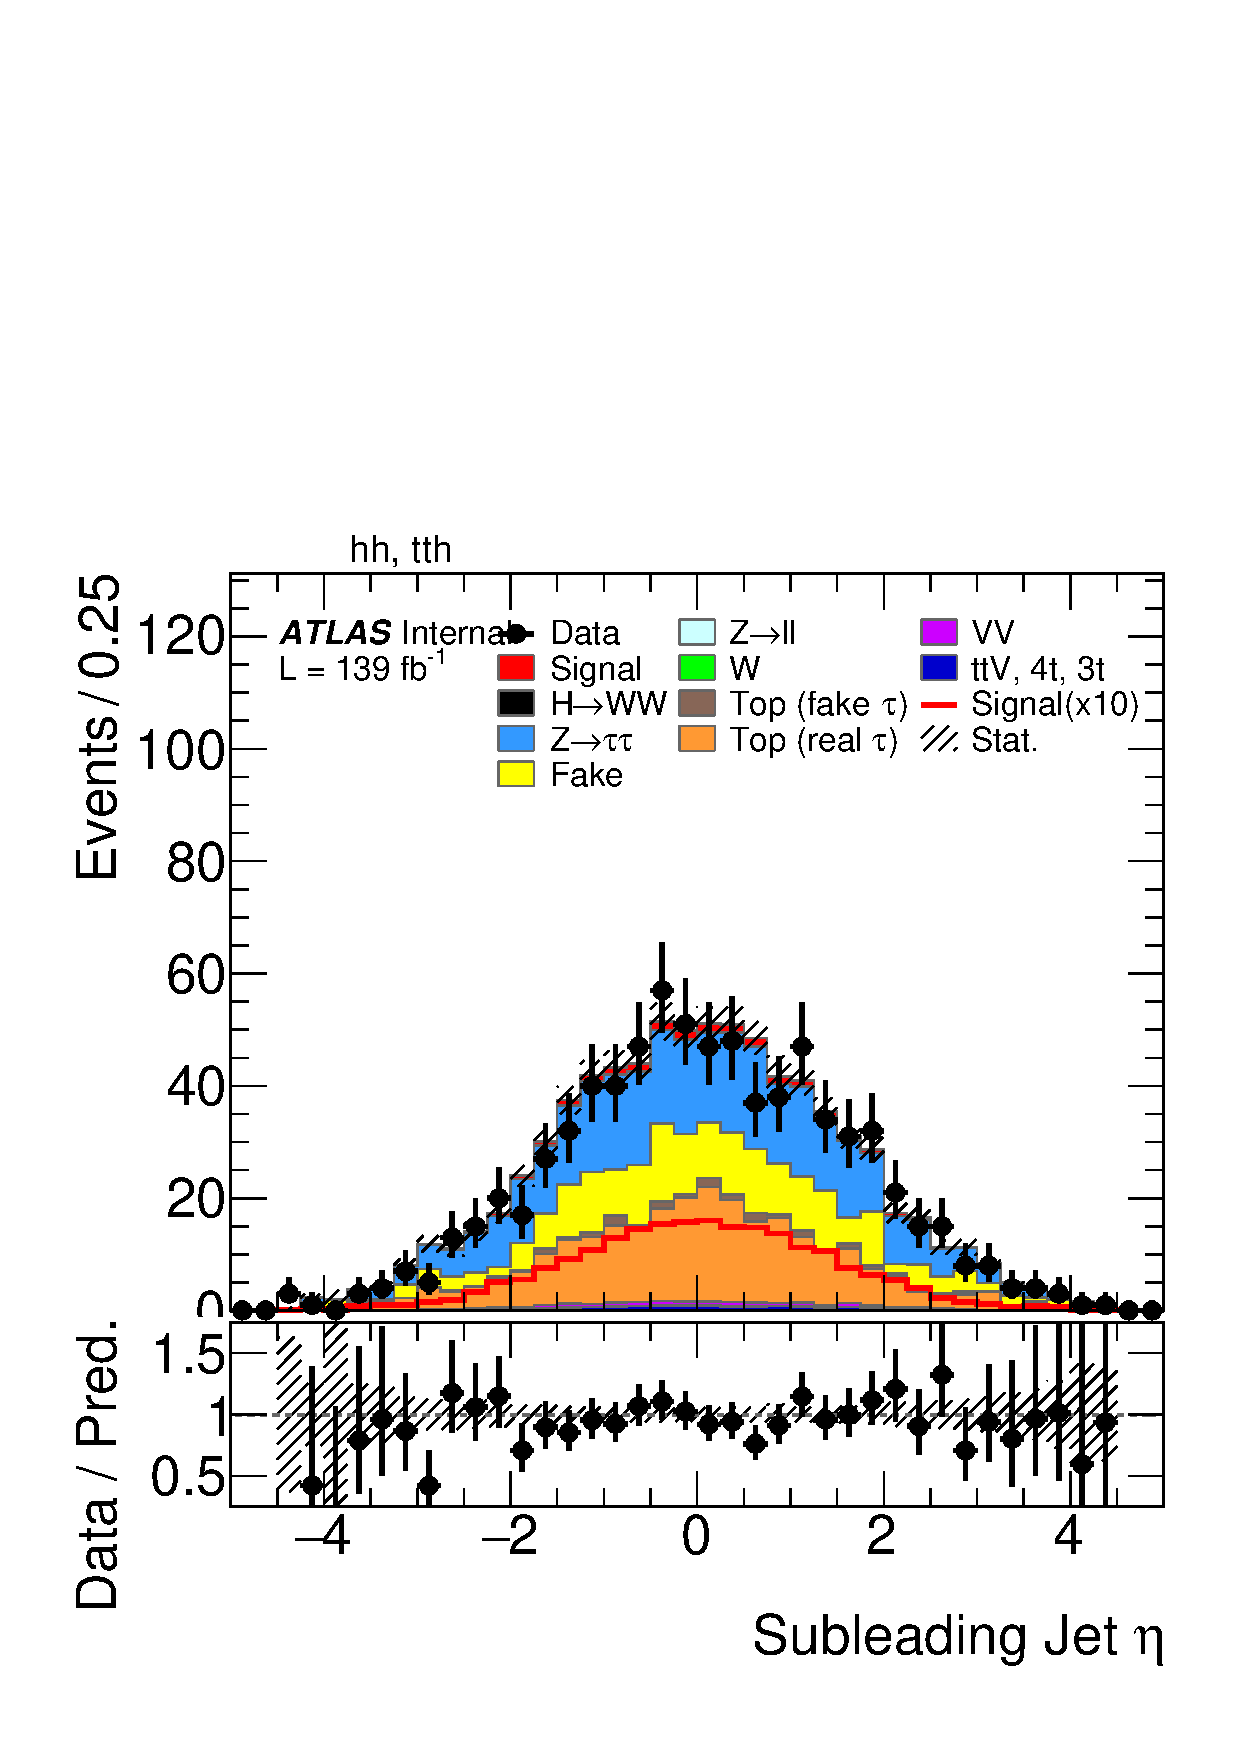
\includegraphics[width=0.33\textwidth]{images/modelling_tmva_vars/plot_jet_1_eta_hh_tth.pdf} &
    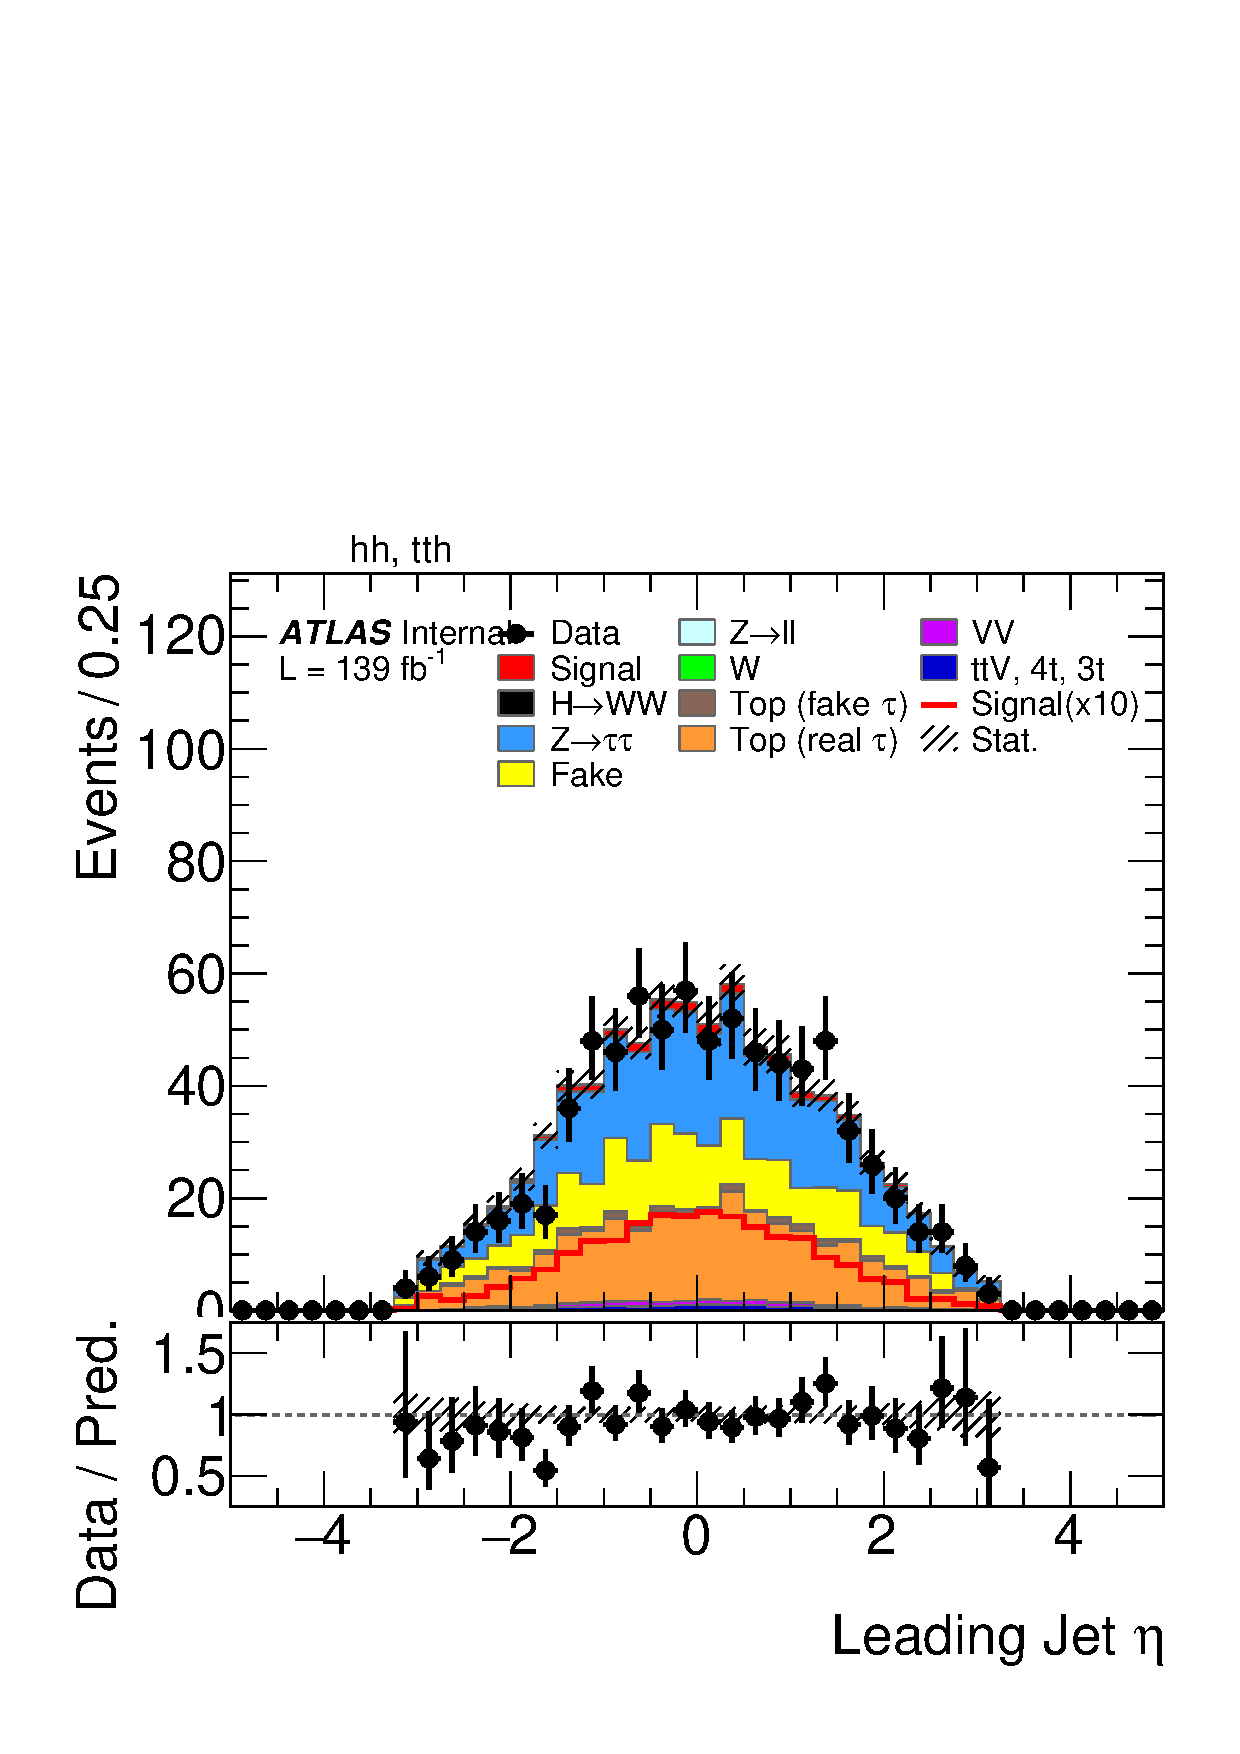
\includegraphics[width=0.33\textwidth]{images/modelling_tmva_vars/plot_jet_0_eta_hh_tth.pdf} &
    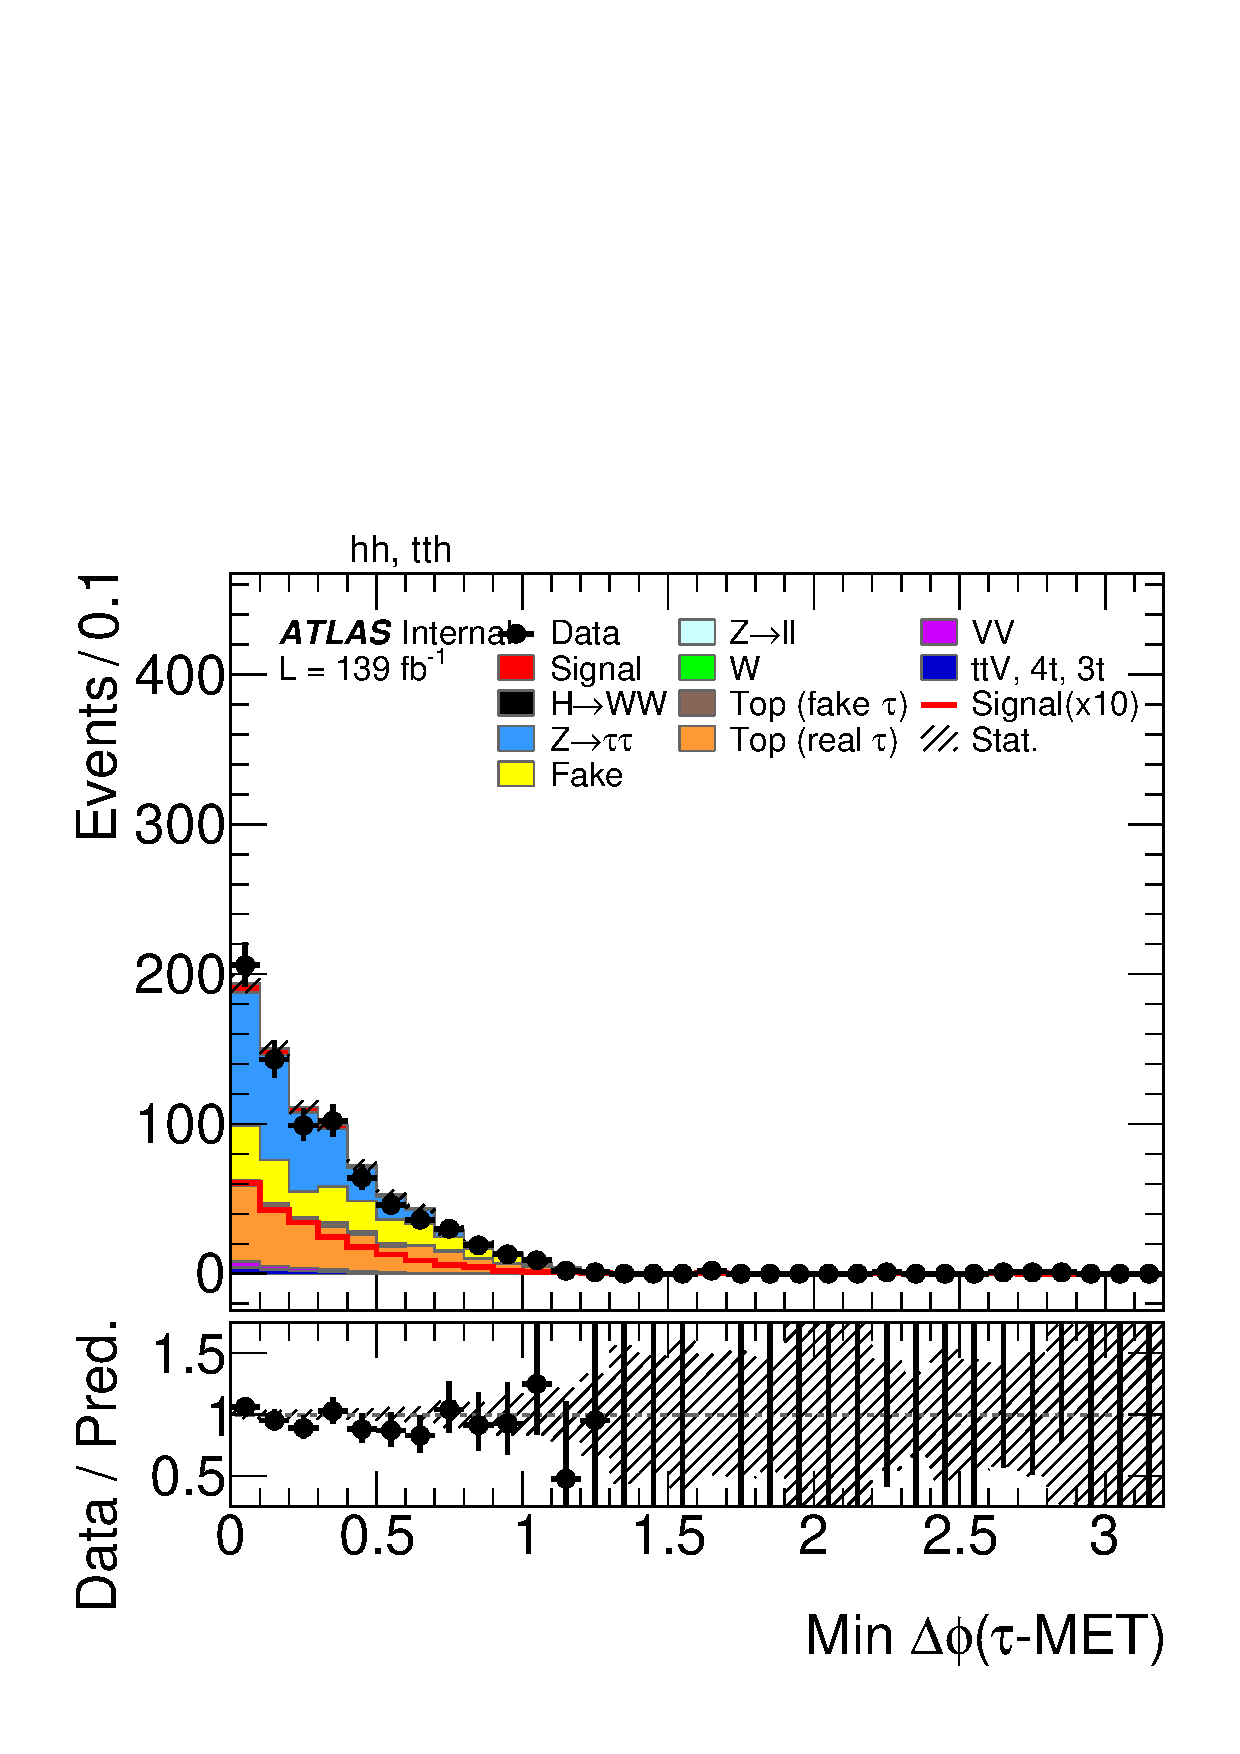
\includegraphics[width=0.33\textwidth]{images/modelling_tmva_vars/plot_ditau_met_min_dphi_hh_tth.pdf}
  \end{tabular}

  \caption{Data/MC modelling for the \ttH BDT input variables at the \ttHtt preselection. Only statistical uncertainties are shown.}
  \label{tth_vars_modelling_2}
\end{figure}

\begin{figure}[htbp]
  \centering
  \setlength{\tabcolsep}{1.5pt}
  \renewcommand{\arraystretch}{0}

  \begin{tabular}{@{}c c c@{}}
    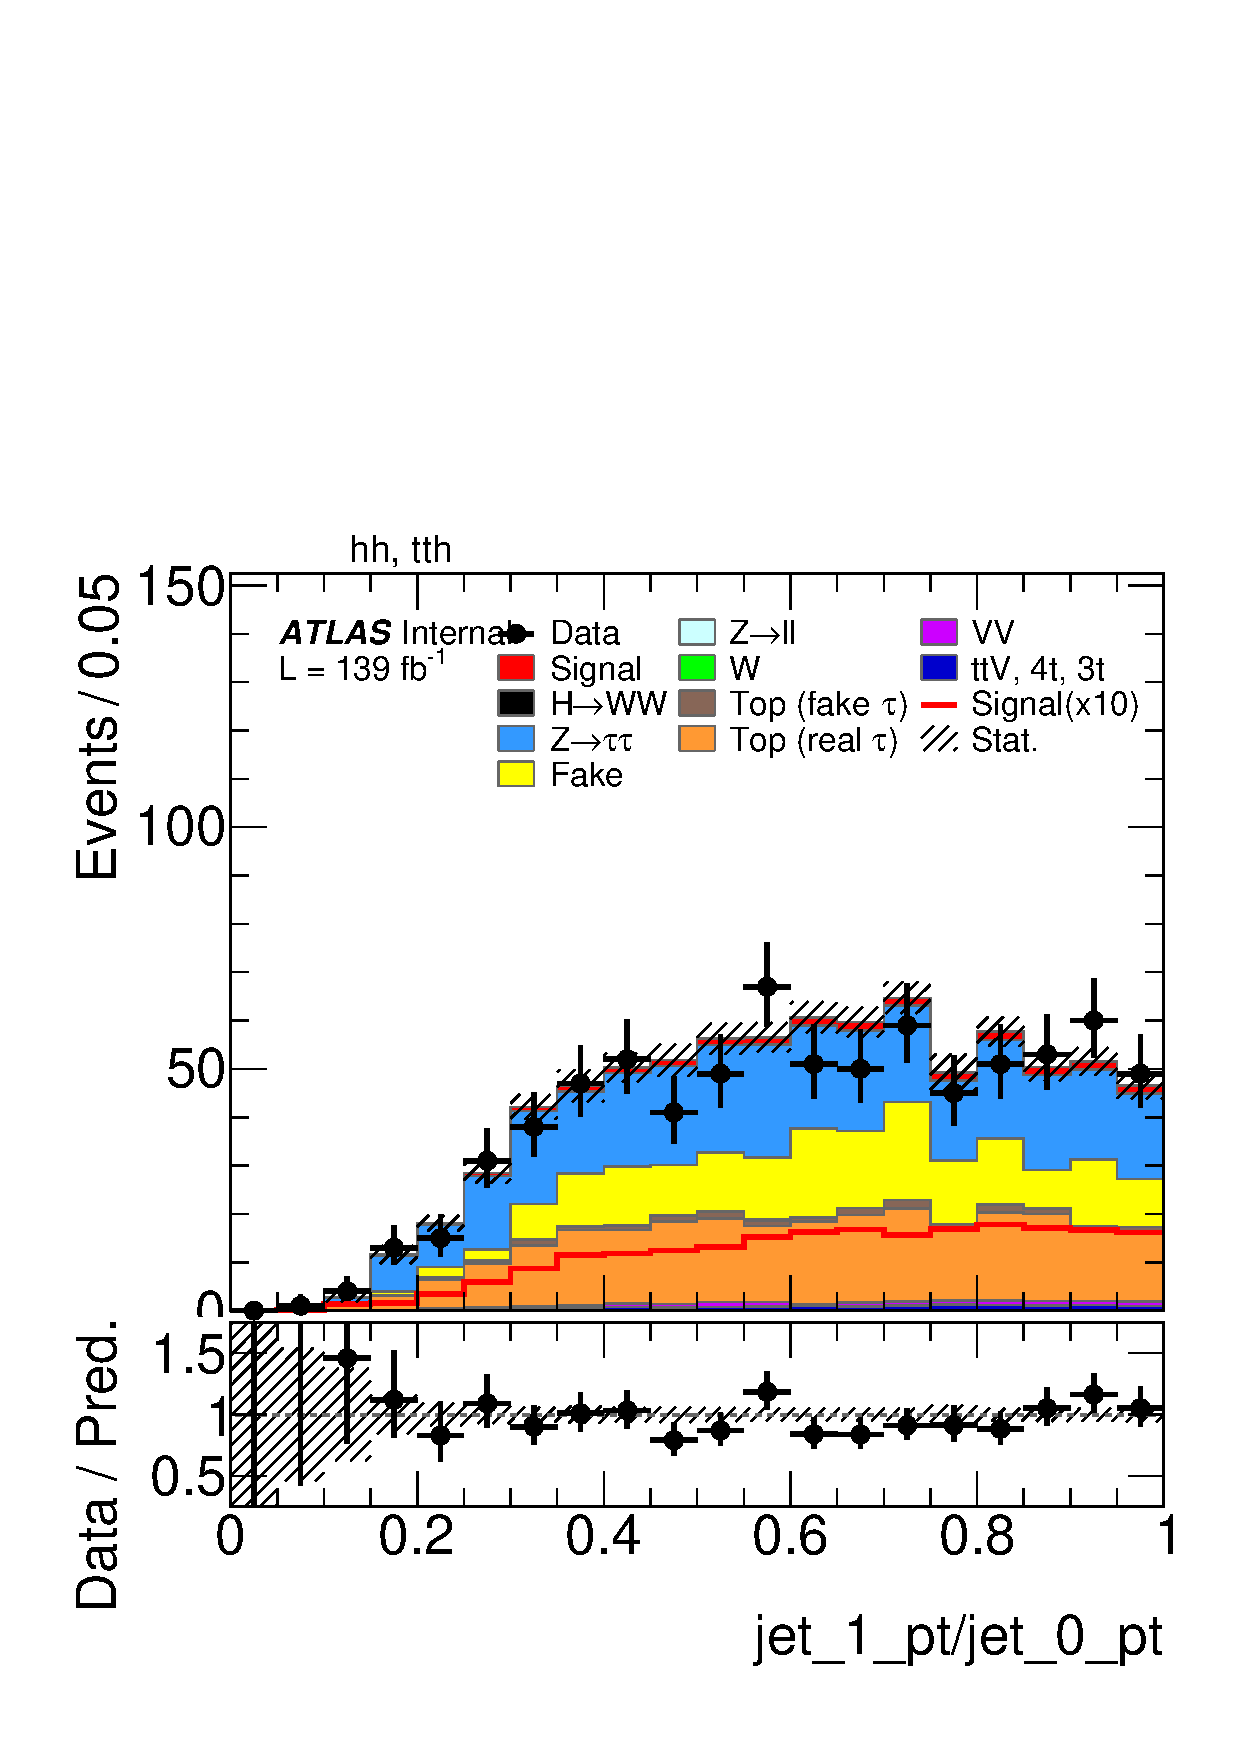
\includegraphics[width=0.33\textwidth]{images/modelling_tmva_vars/plot_ratio01_hh_tth.pdf} &
    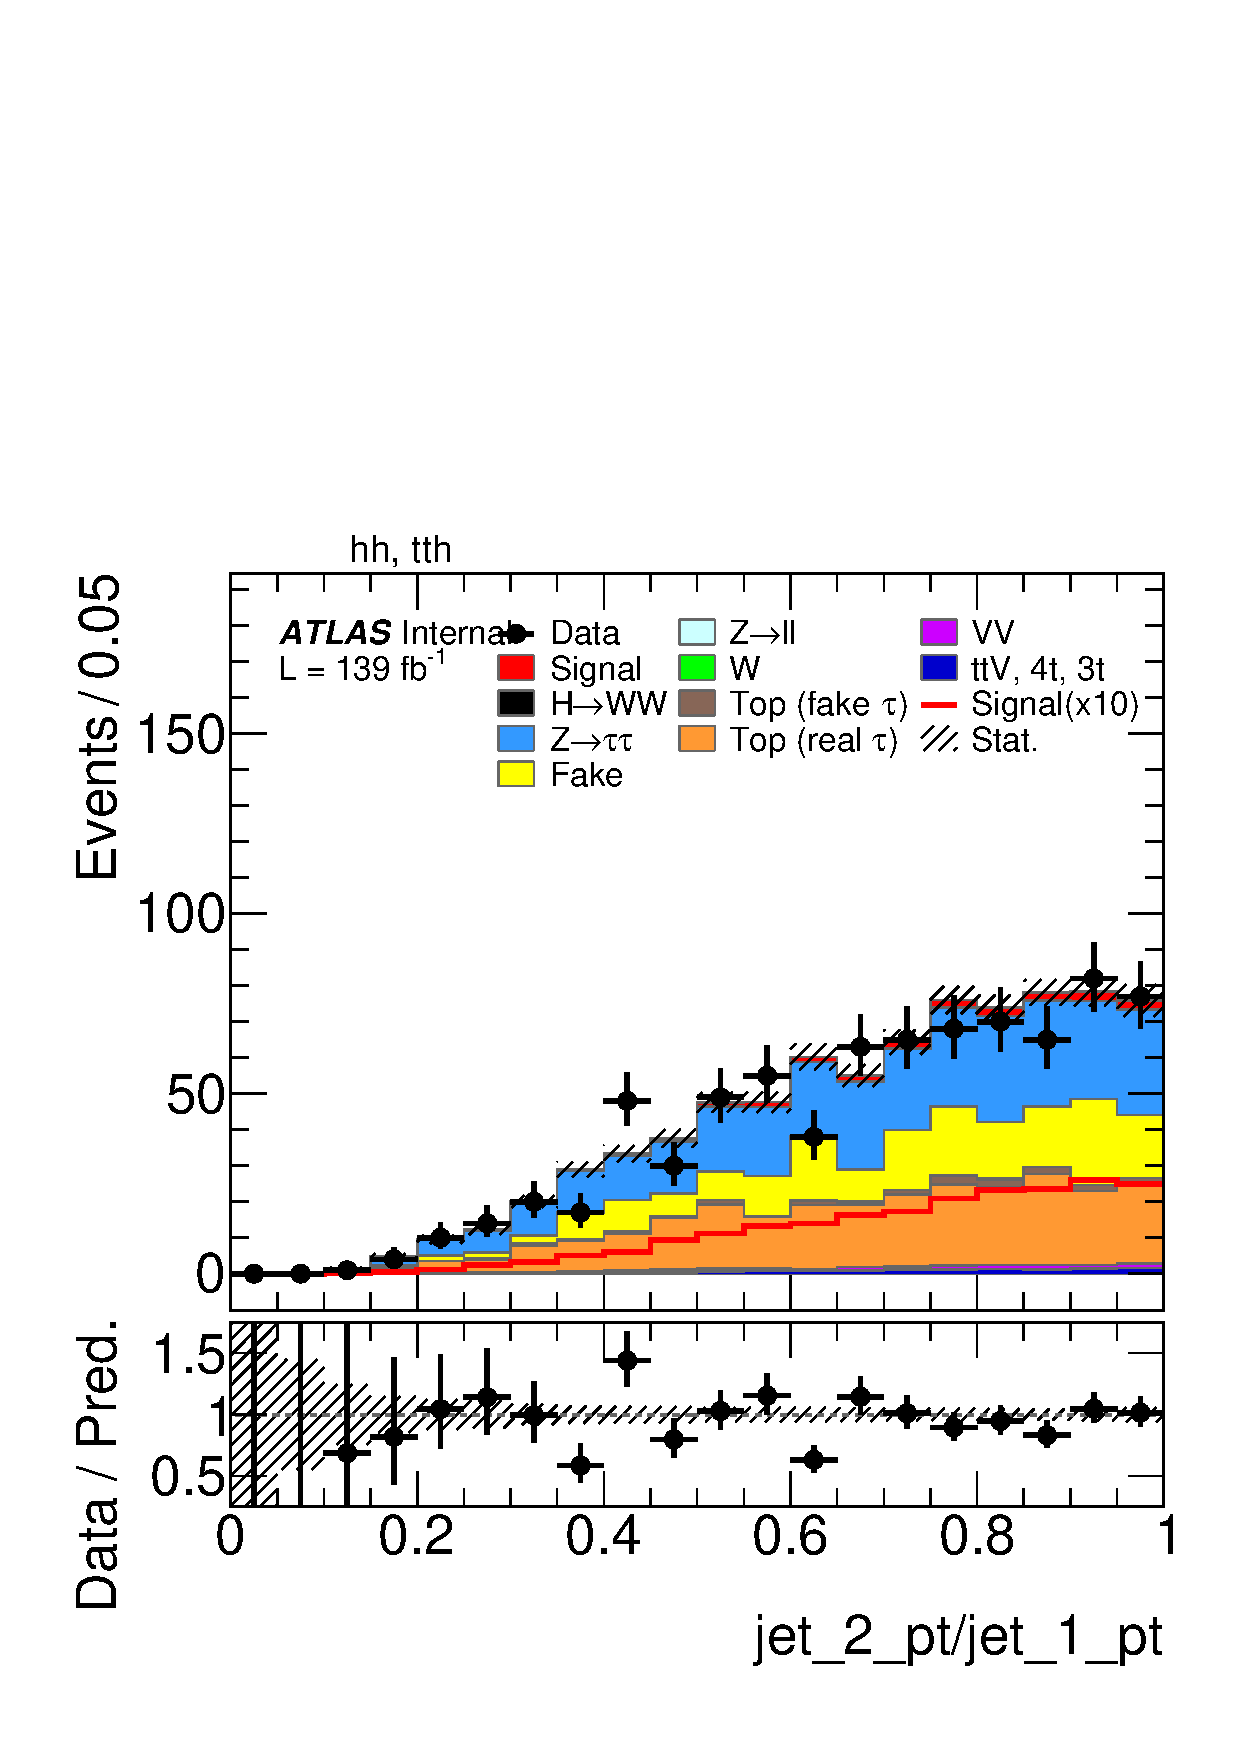
\includegraphics[width=0.33\textwidth]{images/modelling_tmva_vars/plot_ratio12_hh_tth.pdf} &
    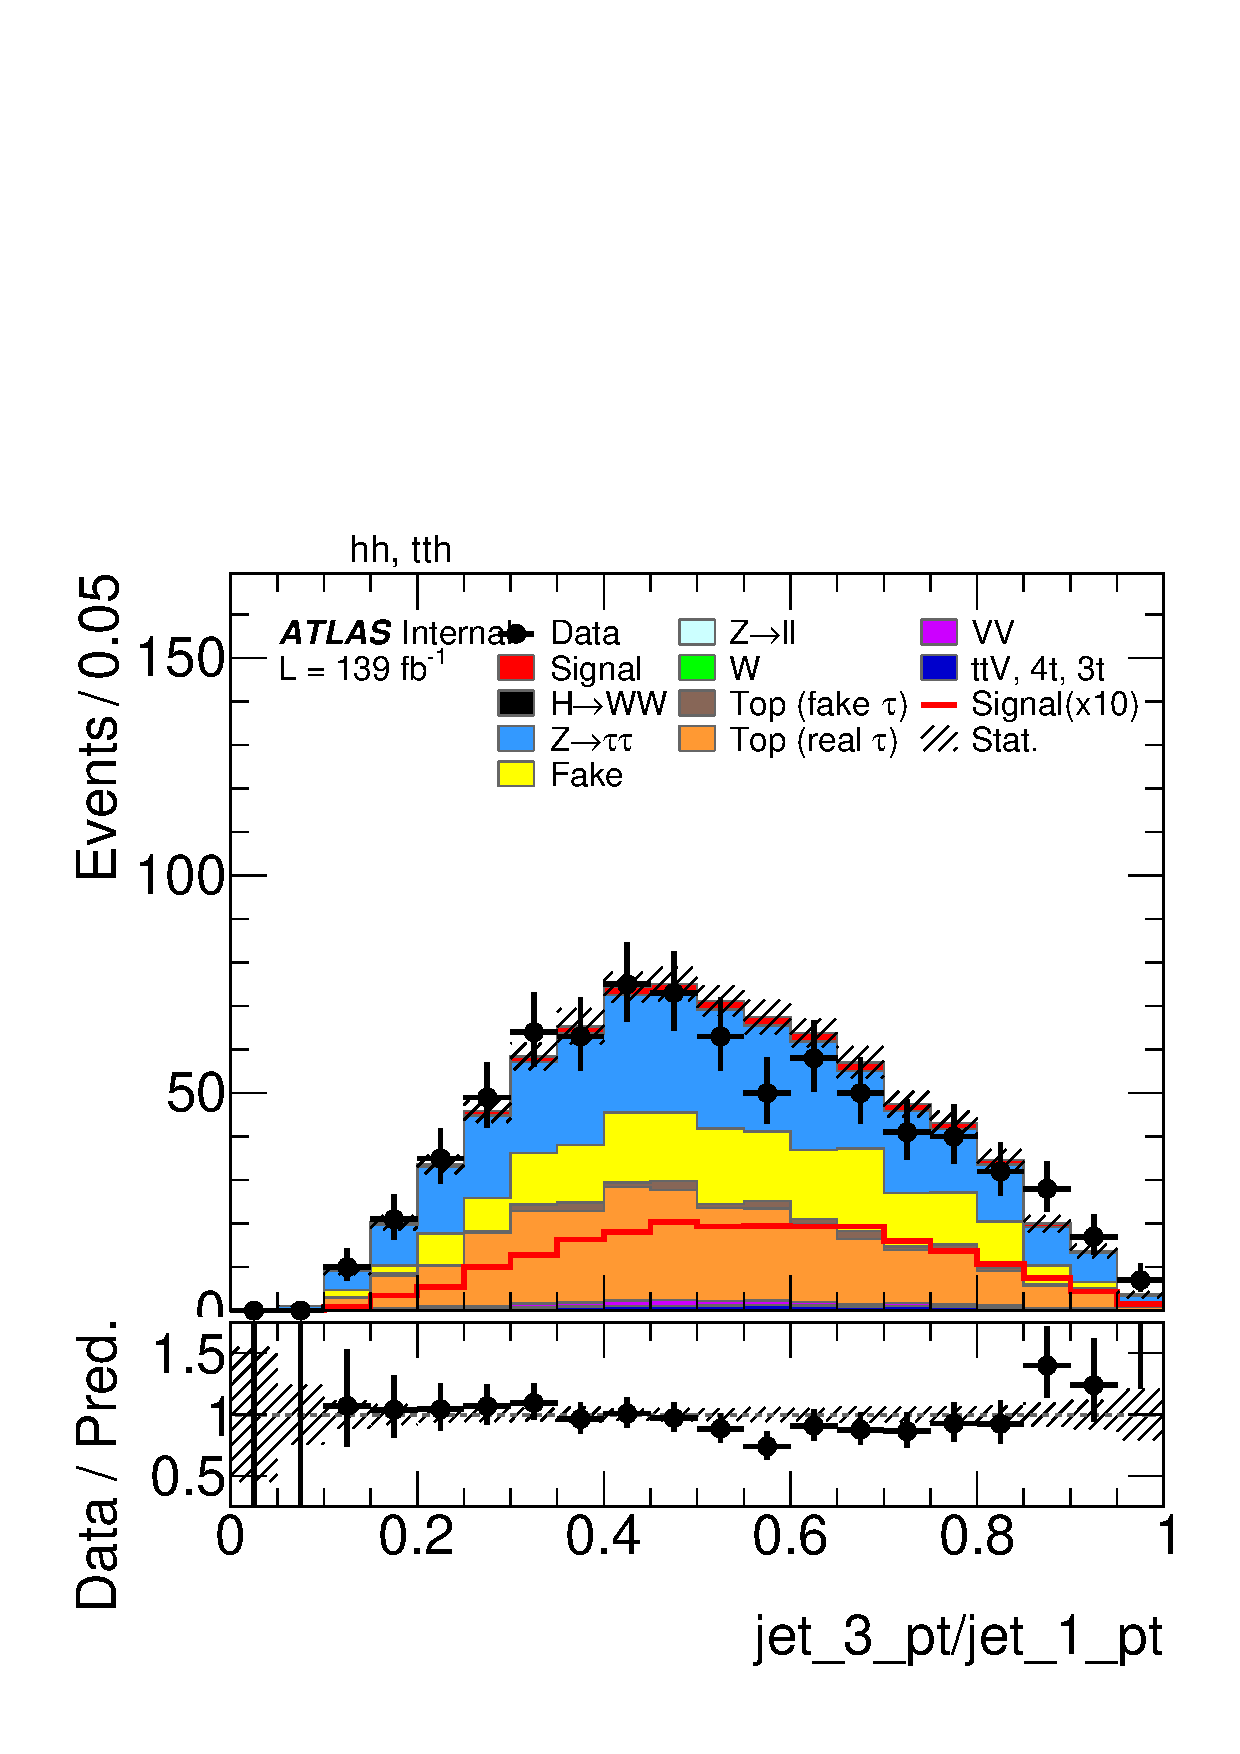
\includegraphics[width=0.33\textwidth]{images/modelling_tmva_vars/plot_ratio13_hh_tth.pdf}
  \end{tabular}

  \caption{Data/MC modelling for the \ttH BDT input variables at the \ttHtt preselection. Only statistical uncertainties are shown.}
  \label{tth_vars_modelling_3}
\end{figure}


\subsection{BDT training}

As already mentioned, in order to more precisely target the STXS phase space bins for this \ttH production mode, two separate BDT trainings are performed with the setup described above. Taking advantage of the NN \pth reconstruction (Section~\ref{sec:higgs_reconstruction}), a ``low-\pth'' training is carried out with events satisfying \pth$<200$~GeV, and a ``high-\pth'' training is implemented using events with \pth$>200$~GeV.  

This strategy is further motivated by the fact that the relative contributions of the two dominant background sources vary as a function of \pth. For instance, most of the \ttbar events populate the region with \pth$<200$~GeV, while at higher values the \ztautau background becomes dominant, as illustrated in Figure~\ref{reconstructed_preselection_b}. It was verified that splitting the training in this way improves the discrimination against the \ttbar background in the low-\pth region, compared to an inclusive training in this variable.

The highest ranked variables in both trainings do not vary significantly, nor do they across the different folds in the cross-validation, as expected. In all cases, the jet $p_{\text{T}}$ ratios and the angular distances between the \tauhadvis candidates are among the most influential observables, together with the pseudorapidity of the leading jets and other jet-related properties. Table~\ref{tab:bdt_importance_high_low} shows the ranking list for both trainings at low and high \pth.

\begin{table}[h]
  \centering
  \scriptsize
  \caption{Ranking of input variables by their importance in the BDT training, shown separately for the (a) high-$p_{\mathrm{T}}^{H}$ and (b) low-$p_{\mathrm{T}}^{H}$ categories. The variable importance, as computed in TMVA, reflects the average separation power of each variable across the ensemble of decision trees.}
  \renewcommand{\arraystretch}{1.05}
  \setlength{\tabcolsep}{2.5pt} % controla el espacio horizontal entre columnas
  \begin{subtable}[t]{0.48\textwidth}
    \centering
    \begin{tabular}{r l c}
      \toprule
      \textbf{Rank} & \textbf{Variable} & \textbf{Importance} \tiny{($10^{-2}$)} \\
      \midrule
       1 & ditau\_dr               & 6.26 \\
       2 & ditau\_pt               & 5.82 \\
       3 & met\_reco\_et           & 5.57 \\
       4 & jet\_0\_eta             & 5.43 \\
       5 & ratio13                 & 5.40 \\
       6 & mTopWbest               & 5.28 \\
       7 & ratio01                 & 5.05 \\
       8 & tau\_eta\_0             & 5.04 \\
       9 & eta2                    & 4.70 \\
      10 & jet\_1\_eta               & 4.66 \\
      11 & eta3                    & 4.49 \\
      12 & eta4                    & 4.46 \\
      13 & HTjets                  & 4.43 \\
      14 & ditau\_deta              & 4.40 \\
      15 & minDRbtau               & 4.35 \\
      16 & SumPtBjet               & 4.32 \\
      17 & ratio12                 & 4.31 \\
      18 & ditau\_met\_min\_dphi      & 4.25 \\
      19 & tau\_pt\_1                & 4.21 \\
      20 & jjdrmin                 & 3.96 \\
      21 & mWbest                  & 3.53 \\
      \bottomrule
    \end{tabular}
    \caption{High-$p_{\mathrm{T}}^{H}$ training}
  \end{subtable}%
  \hfill
  \begin{subtable}[t]{0.48\textwidth}
    \centering
    \begin{tabular}{r l c}
      \toprule
      \textbf{Rank} & \textbf{Variable} & \textbf{Importance} \tiny{($10^{-2}$)} \\
      \midrule
       1 & ditau\_dr             & 6.14 \\
       2 & ratio13               & 5.64 \\
       3 & jet\_0\_eta           & 5.54 \\
       4 & met\_reco\_et         & 5.52 \\
       5 & ditau\_pt             & 5.48 \\
       6 & mTopWbest             & 5.36 \\
       7 & ratio01               & 5.14 \\
       8 & tau\_eta\_0           & 5.10 \\
       9 & jet\_1\_eta           & 4.68 \\
      10 & eta2                  & 4.64 \\
      11 & ditau\_deta           & 4.61 \\
      12 & eta3                  & 4.59 \\
      13 & ratio12               & 4.58 \\
      14 & eta4                  & 4.56 \\
      15 & HTjets                & 4.48 \\
      16 & ditau\_met\_min\_dphi & 4.39 \\
      17 & tau\_pt\_1            & 4.28 \\
      18 & SumPtBjet             & 4.24 \\
      19 & minDRbtau             & 3.90 \\
      20 & jjdrmin              & 3.75 \\
      21 & mWbest                & 3.45 \\
      \bottomrule
    \end{tabular}
    \caption{Low-$p_{\mathrm{T}}^{H}$ training}
  \end{subtable}
  \label{tab:bdt_importance_high_low}
\end{table}

The expected distributions of the three BDT scores obtained for both trainings are shown in Figures~\ref{lowpt_scores} and~\ref{highpt_scores}, corresponding to the low- and high-\pth trainings, respectively. These distributions are evaluated on the training sample, represented by coloured markers, and on the testing sample, shown as boxes, allowing us to assess the level of overtraining. The effect is not particularly pronounced, although it is more visible in the low-\pth case due to the smaller statistics and the presence of larger fluctuations.  

From Figure~\ref{lowpt_scores} it can be seen that, at low \pth, the BDT focuses primarily on the identification of \ttbar events, also because the available statistics for \ttHtt and \ztautau are smaller. In contrast, Figure~\ref{highpt_scores} shows that at high \pth the discrimination of signal and of the \ztautau background is enhanced. Ideally, the score of each class is expected to peak around unity for events of its own class and to be close to zero for the others, bearing in mind that the outputs are normalised in both trainings.
\begin{figure}[htbp]
  \centering
  \setlength{\tabcolsep}{1.5pt}
  \renewcommand{\arraystretch}{0}
  \begin{tabular}{@{}c c c@{}}
    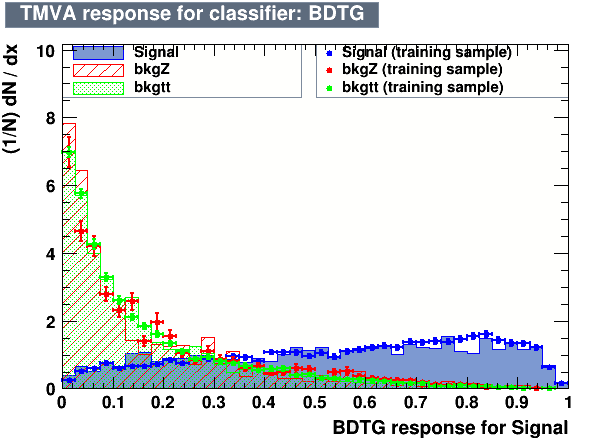
\includegraphics[width=0.33\textwidth]{images/plots_overtrain_lt200/overtrain_Signal_BDTG.png} &
    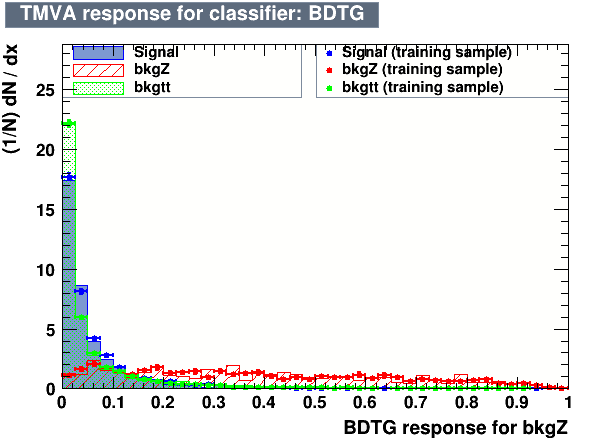
\includegraphics[width=0.33\textwidth]{images/plots_overtrain_lt200/overtrain_bkgZ_BDTG.png} &  
    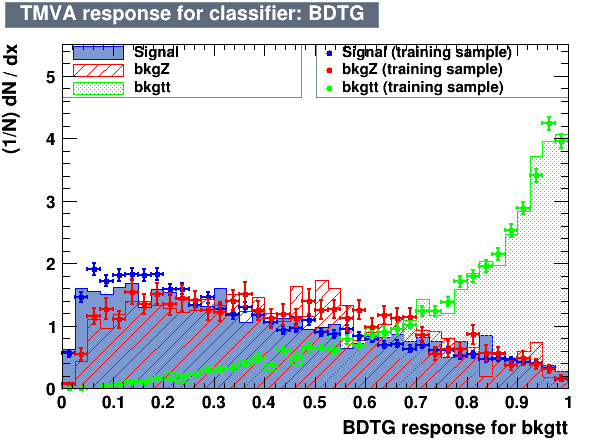
\includegraphics[width=0.33\textwidth]{images/plots_overtrain_lt200/overtrain_bkgtt_BDTG.png}
  \end{tabular}
  \caption{Multiclass BDT score distributions for the low \pth training.}
  \label{lowpt_scores}
\end{figure}

\begin{figure}[htbp]
  \centering
  \setlength{\tabcolsep}{1.5pt}
  \renewcommand{\arraystretch}{0}
  \begin{tabular}{@{}c c c@{}}
    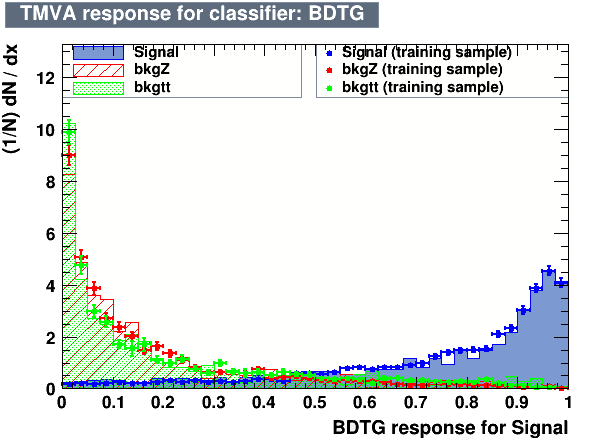
\includegraphics[width=0.33\textwidth]{images/plots_overtrain_gt200/overtrain_Signal_BDTG.png} &
    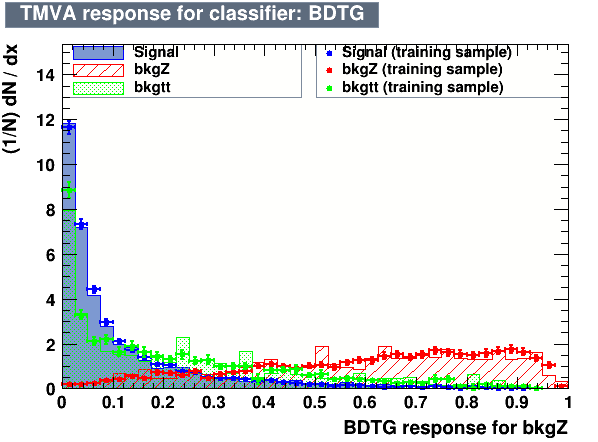
\includegraphics[width=0.33\textwidth]{images/plots_overtrain_gt200/overtrain_bkgZ_BDTG.png} &  
    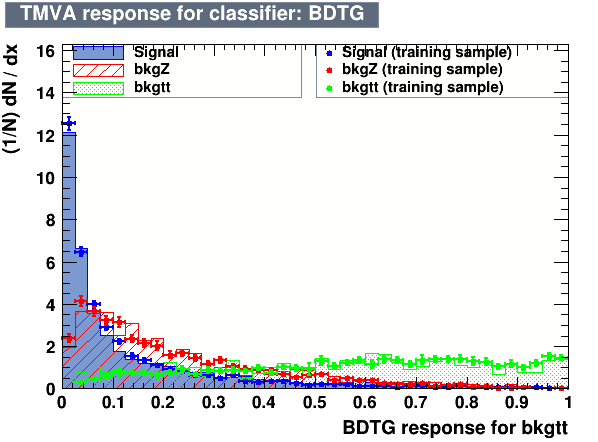
\includegraphics[width=0.33\textwidth]{images/plots_overtrain_gt200/overtrain_bkgtt_BDTG.png}
  \end{tabular}
  \caption{Multiclass BDT score distributions for the high \pth training.}
  \label{highpt_scores}
\end{figure}


As a final step, since the discriminants in both \pth regions will be used to define the analysis categories entering the final statistical fit, it is necessary to confirm that these variables are correctly modelled and that good agreement is observed between data and MC. Figures~\ref{lowpt_modelling} and~\ref{highpt_modelling} show the score distributions of both trainings, comparing collision data with MC simulations at the \ttH preselection level. A good level of agreement is observed between the data and the estimated backgrounds.

\begin{figure}[htbp]
  \centering
  \setlength{\tabcolsep}{1.5pt}
  \renewcommand{\arraystretch}{0}
  \begin{tabular}{@{}c c c@{}}
    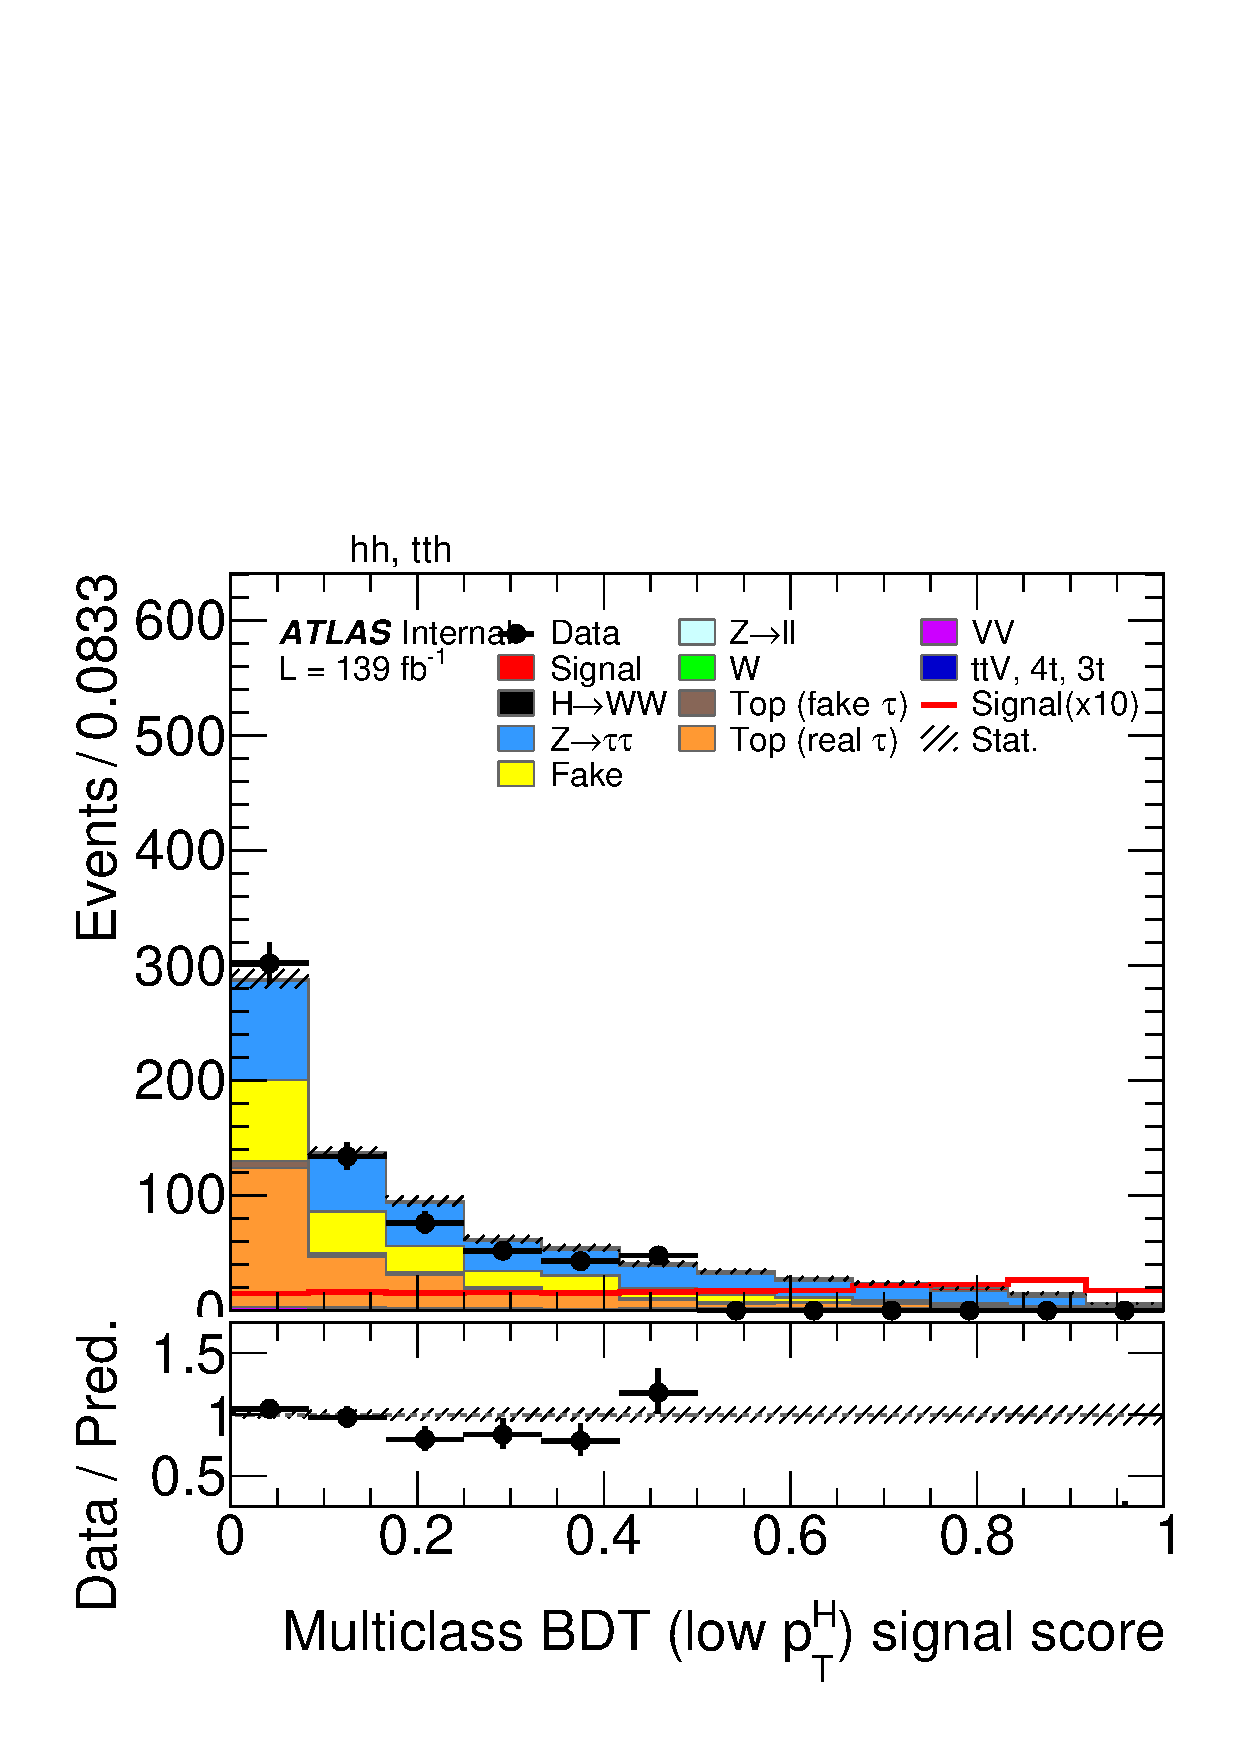
\includegraphics[width=0.32\textwidth]{images/plots_overtrain_lt200/plot_tth_signal_multiclass_lt200_hh_tth.pdf} &
    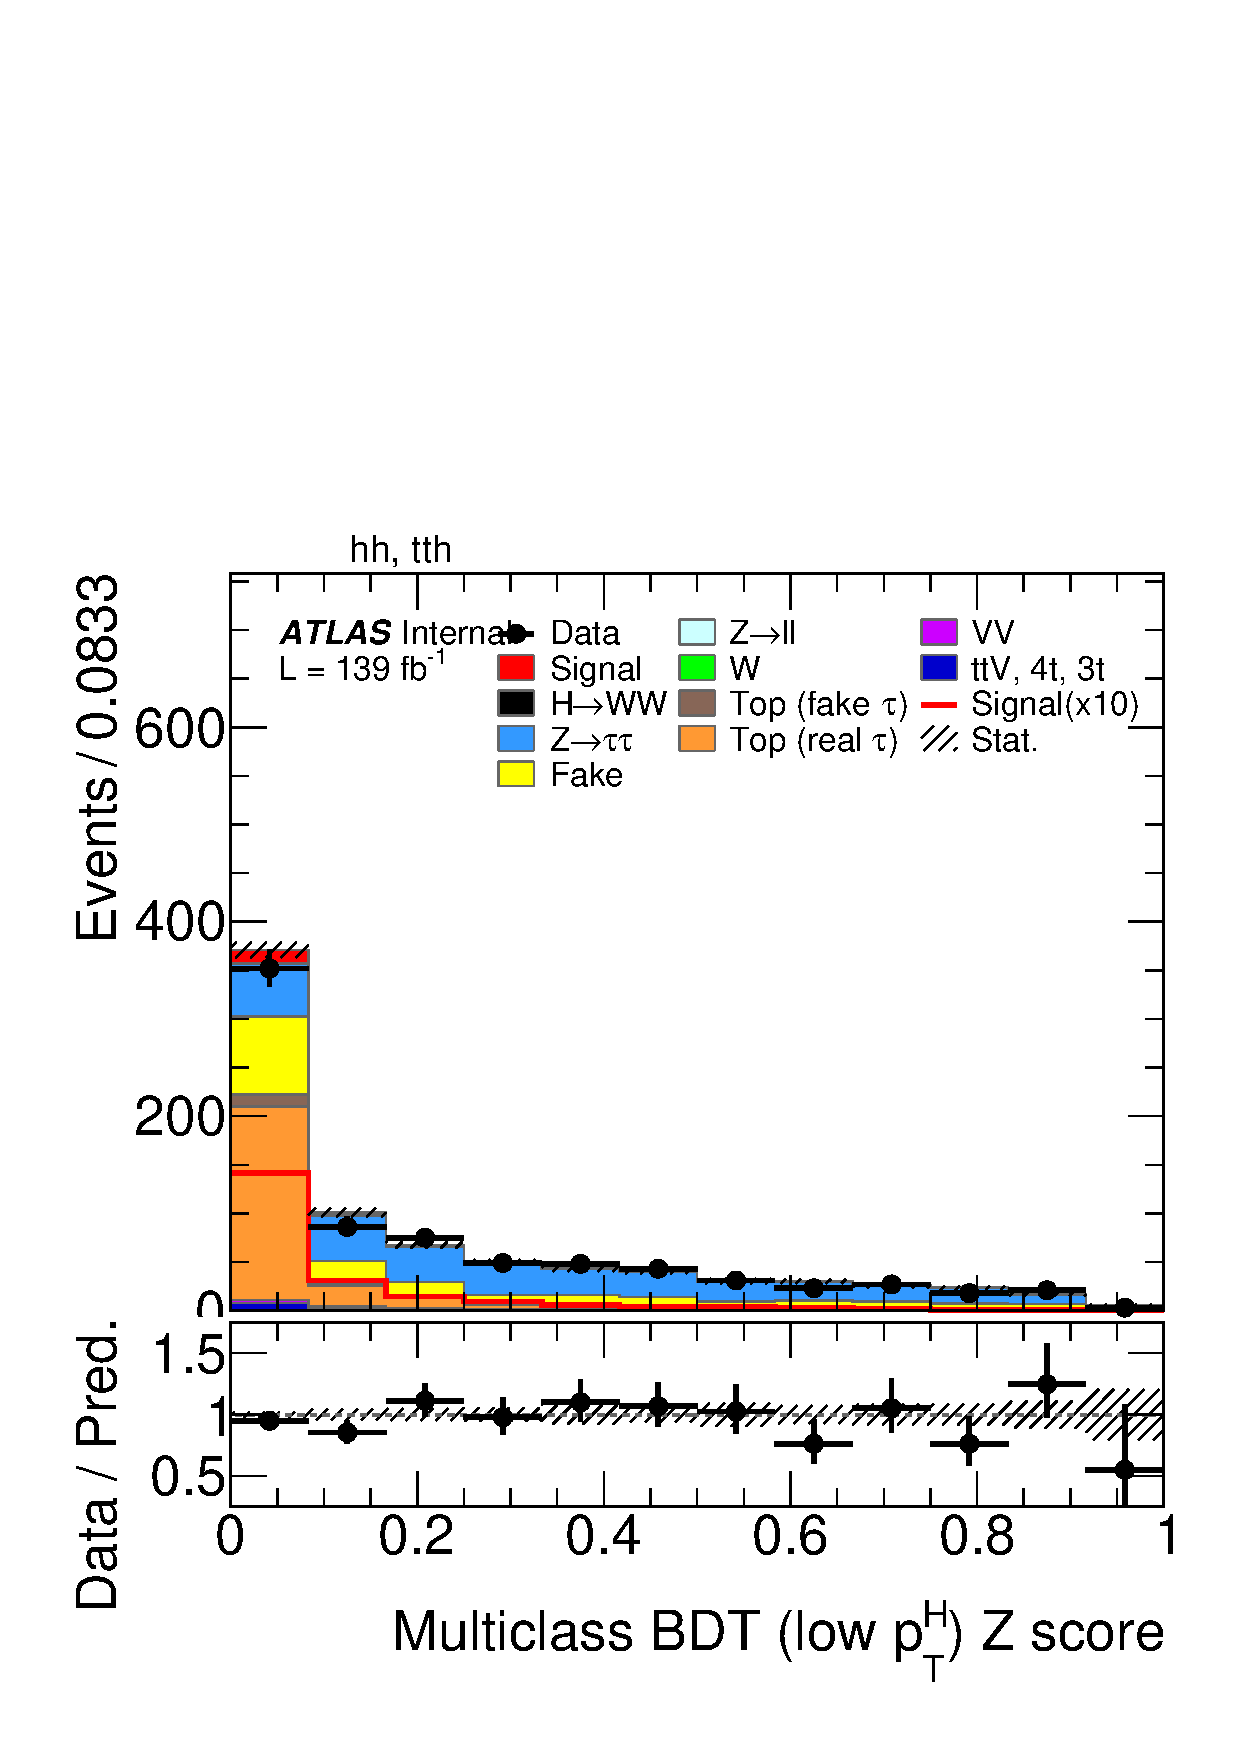
\includegraphics[width=0.32\textwidth]{images/plots_overtrain_lt200/plot_tth_Z_multiclass_lt200_hh_tth.pdf} &  
    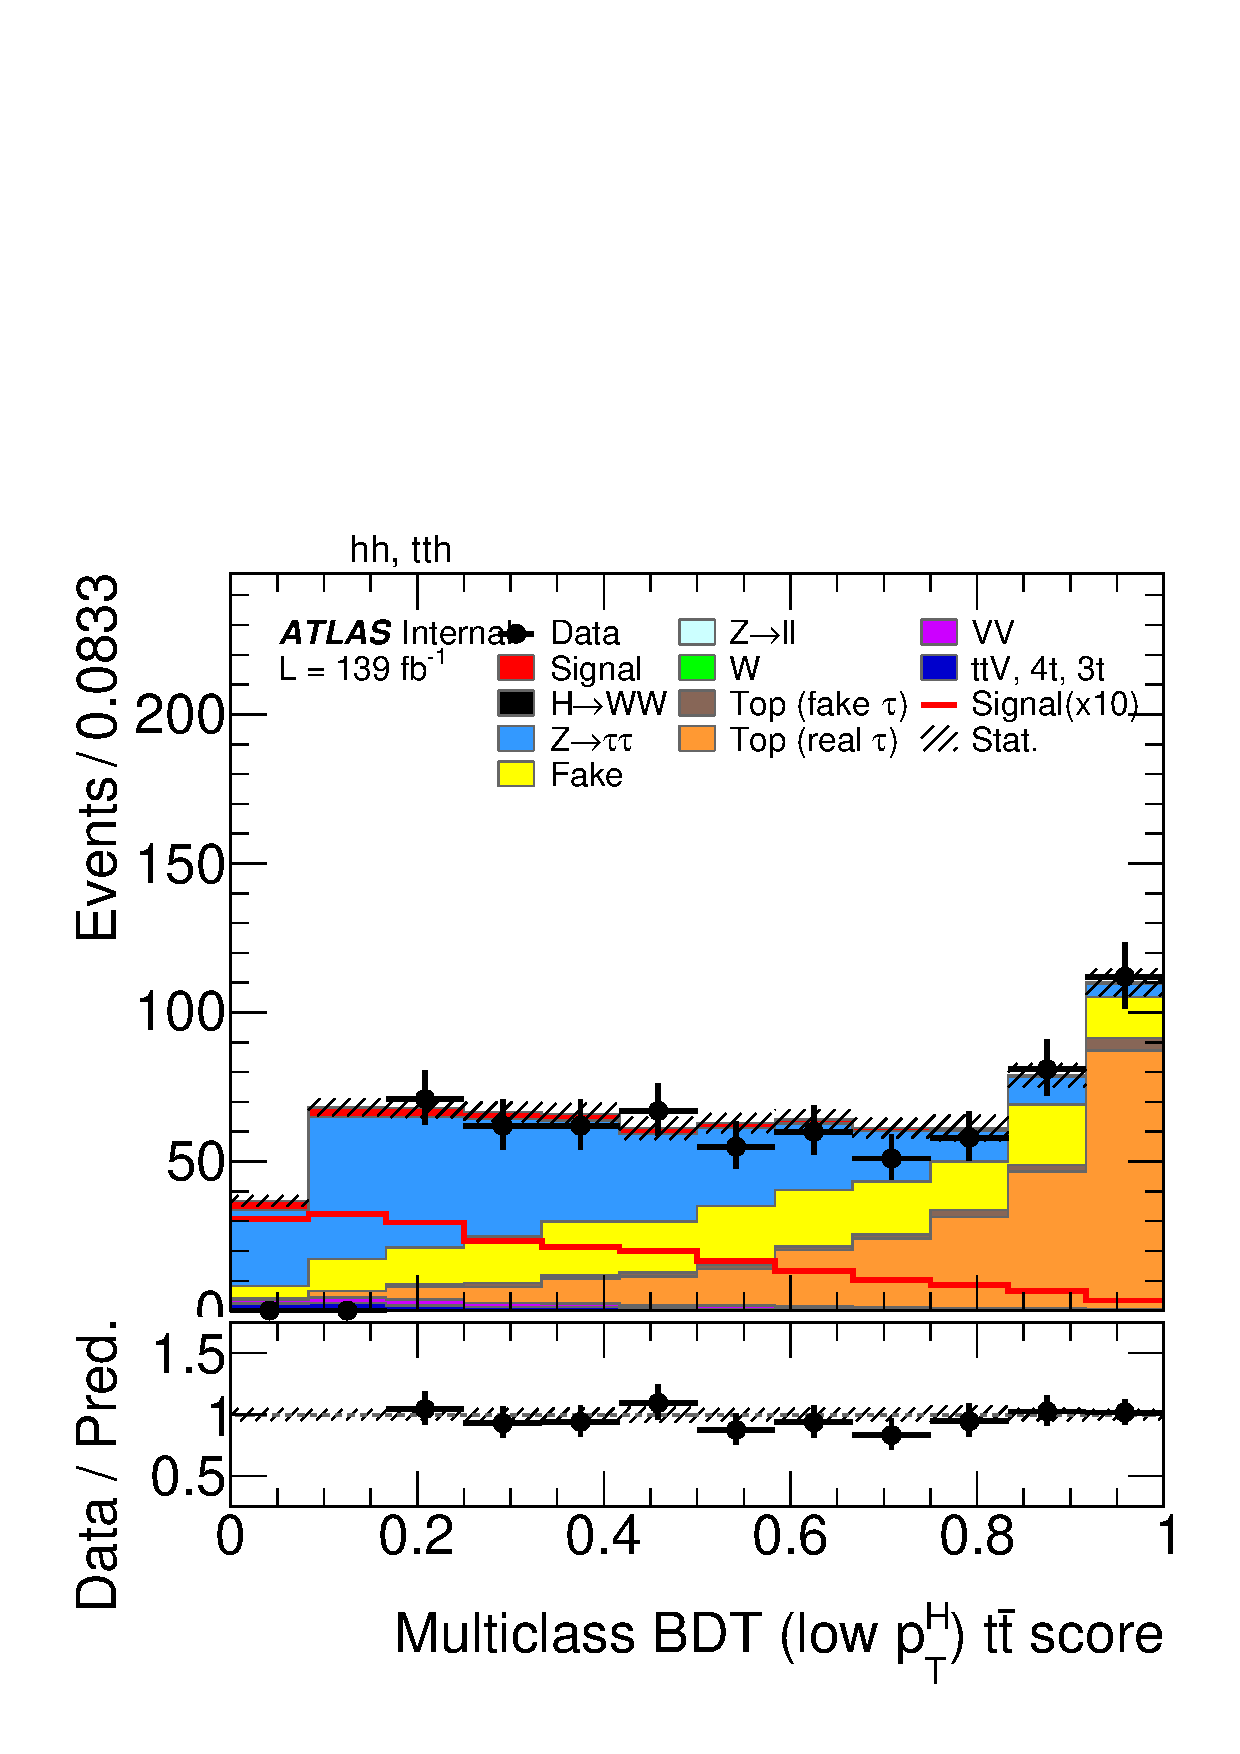
\includegraphics[width=0.32\textwidth]{images/plots_overtrain_lt200/plot_tth_ttbar_multiclass_lt200_hh_tth.pdf}   
  \end{tabular}
  \caption{Multiclass BDT score distributions for the low \pth training.}
  \label{lowpt_modelling}
\end{figure}

\begin{figure}[htbp]
  \centering
  \setlength{\tabcolsep}{1.5pt}
  \renewcommand{\arraystretch}{0}
  \begin{tabular}{@{}c c c@{}}
    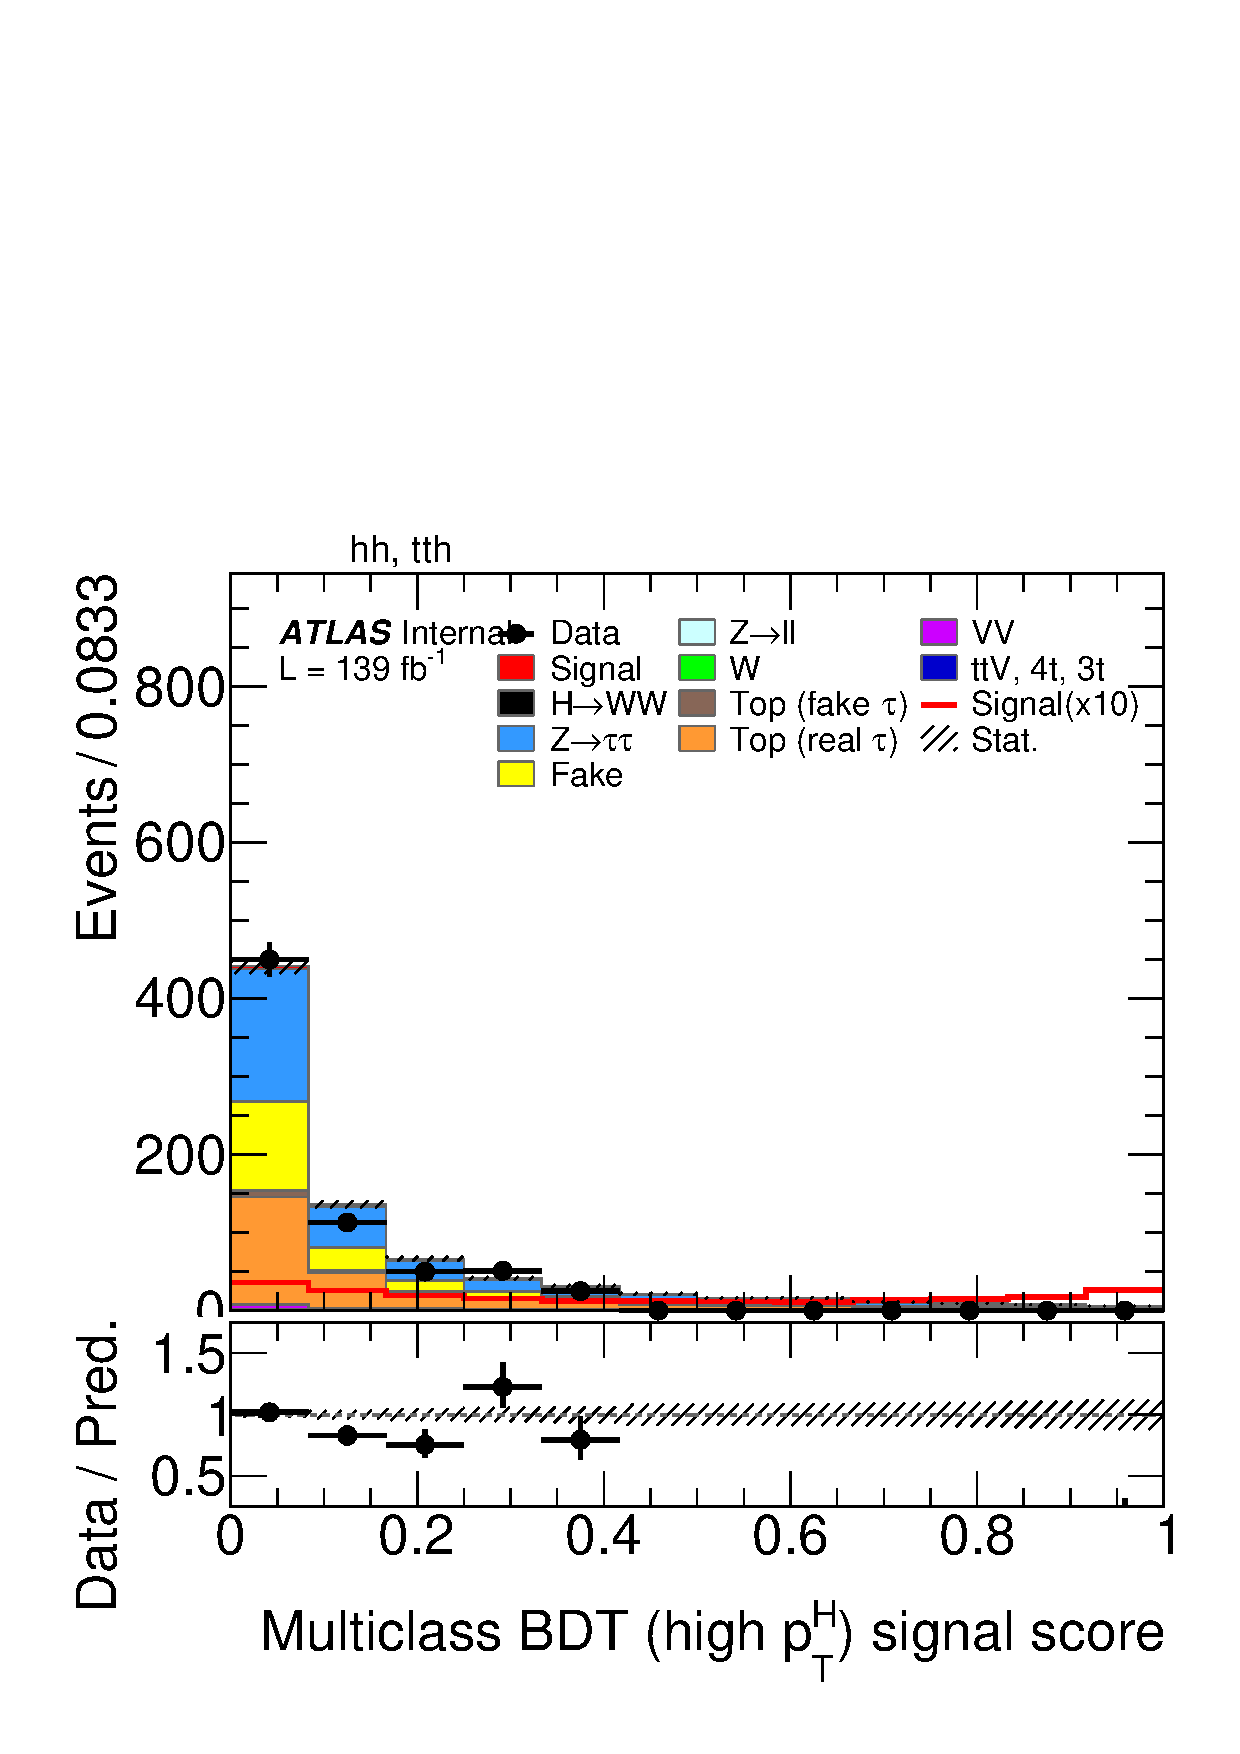
\includegraphics[width=0.32\textwidth]{images/plots_overtrain_gt200/plot_tth_signal_multiclass_gt200_hh_tth.pdf} &
    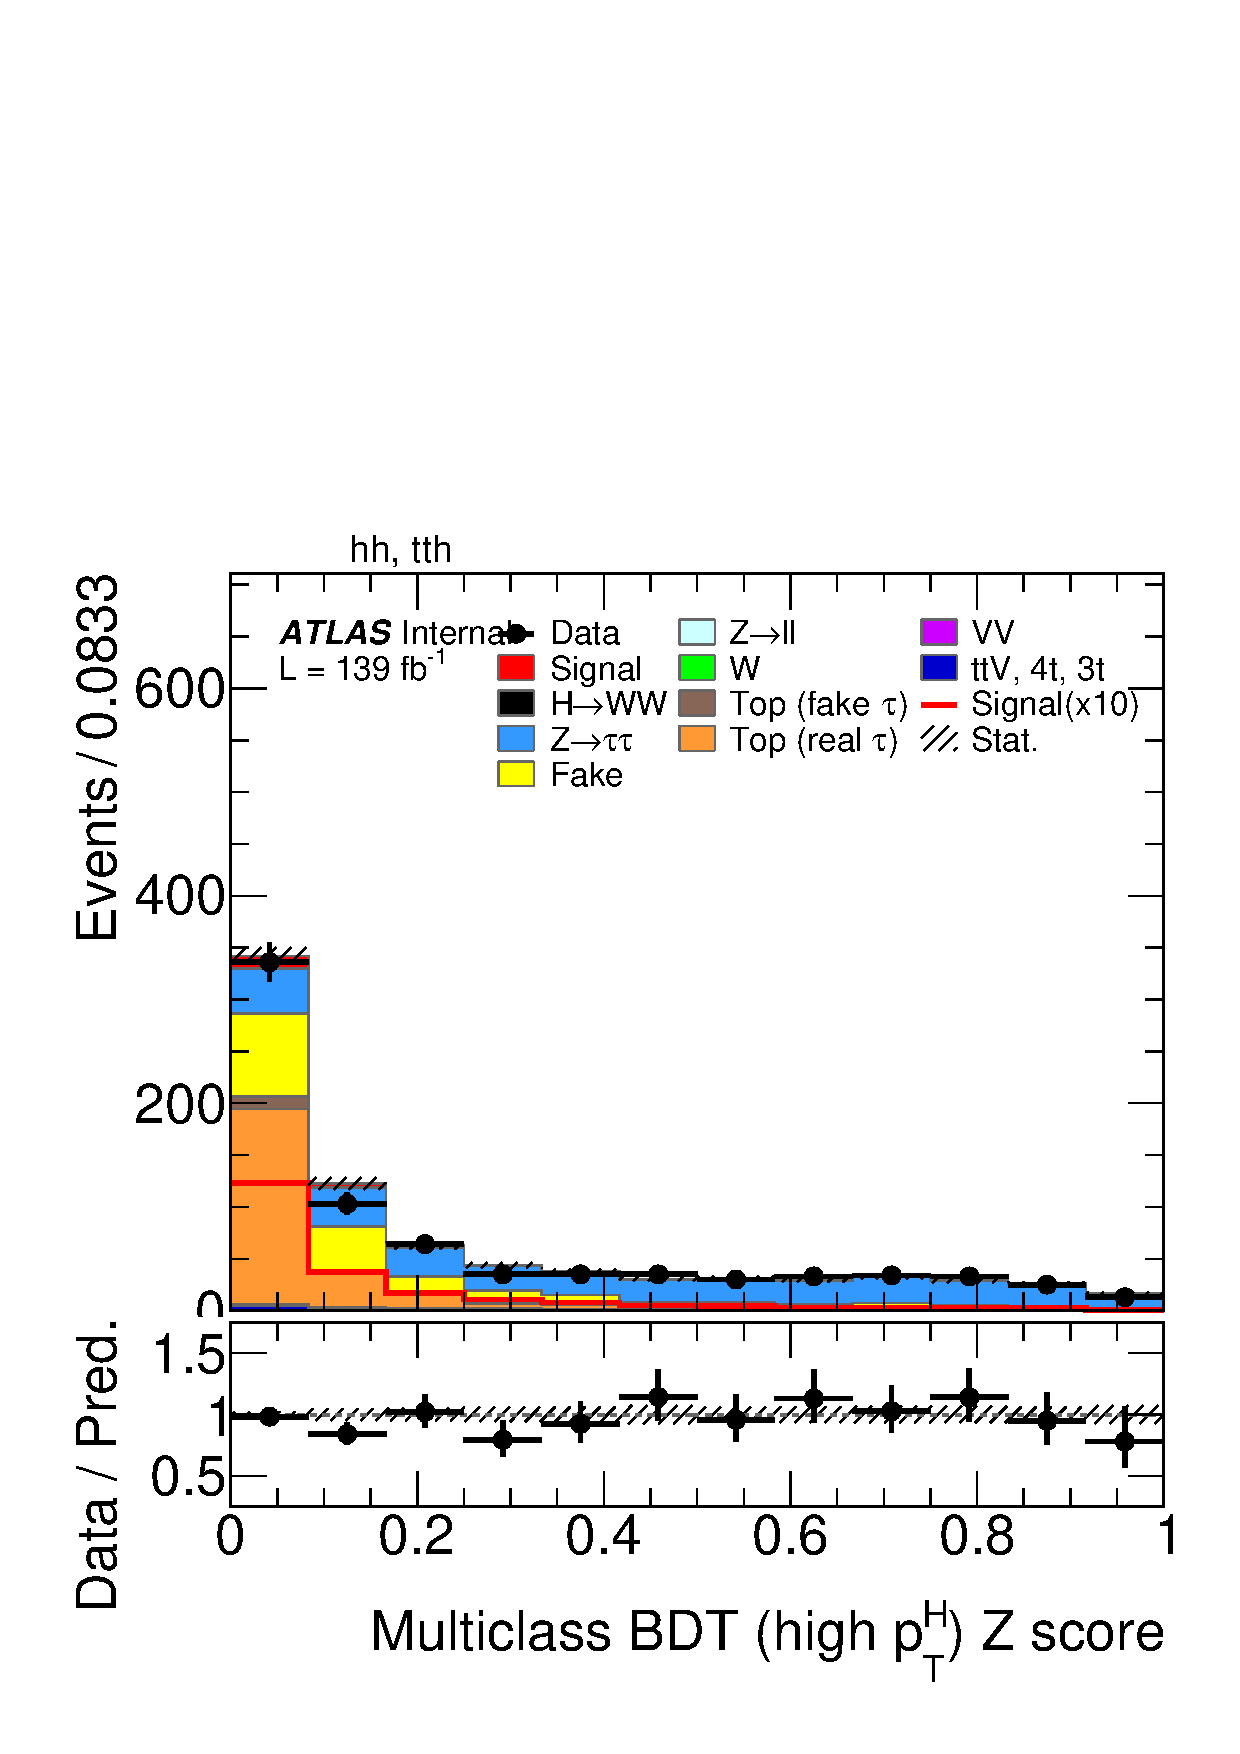
\includegraphics[width=0.32\textwidth]{images/plots_overtrain_gt200/plot_tth_Z_multiclass_gt200_hh_tth.pdf} &  
    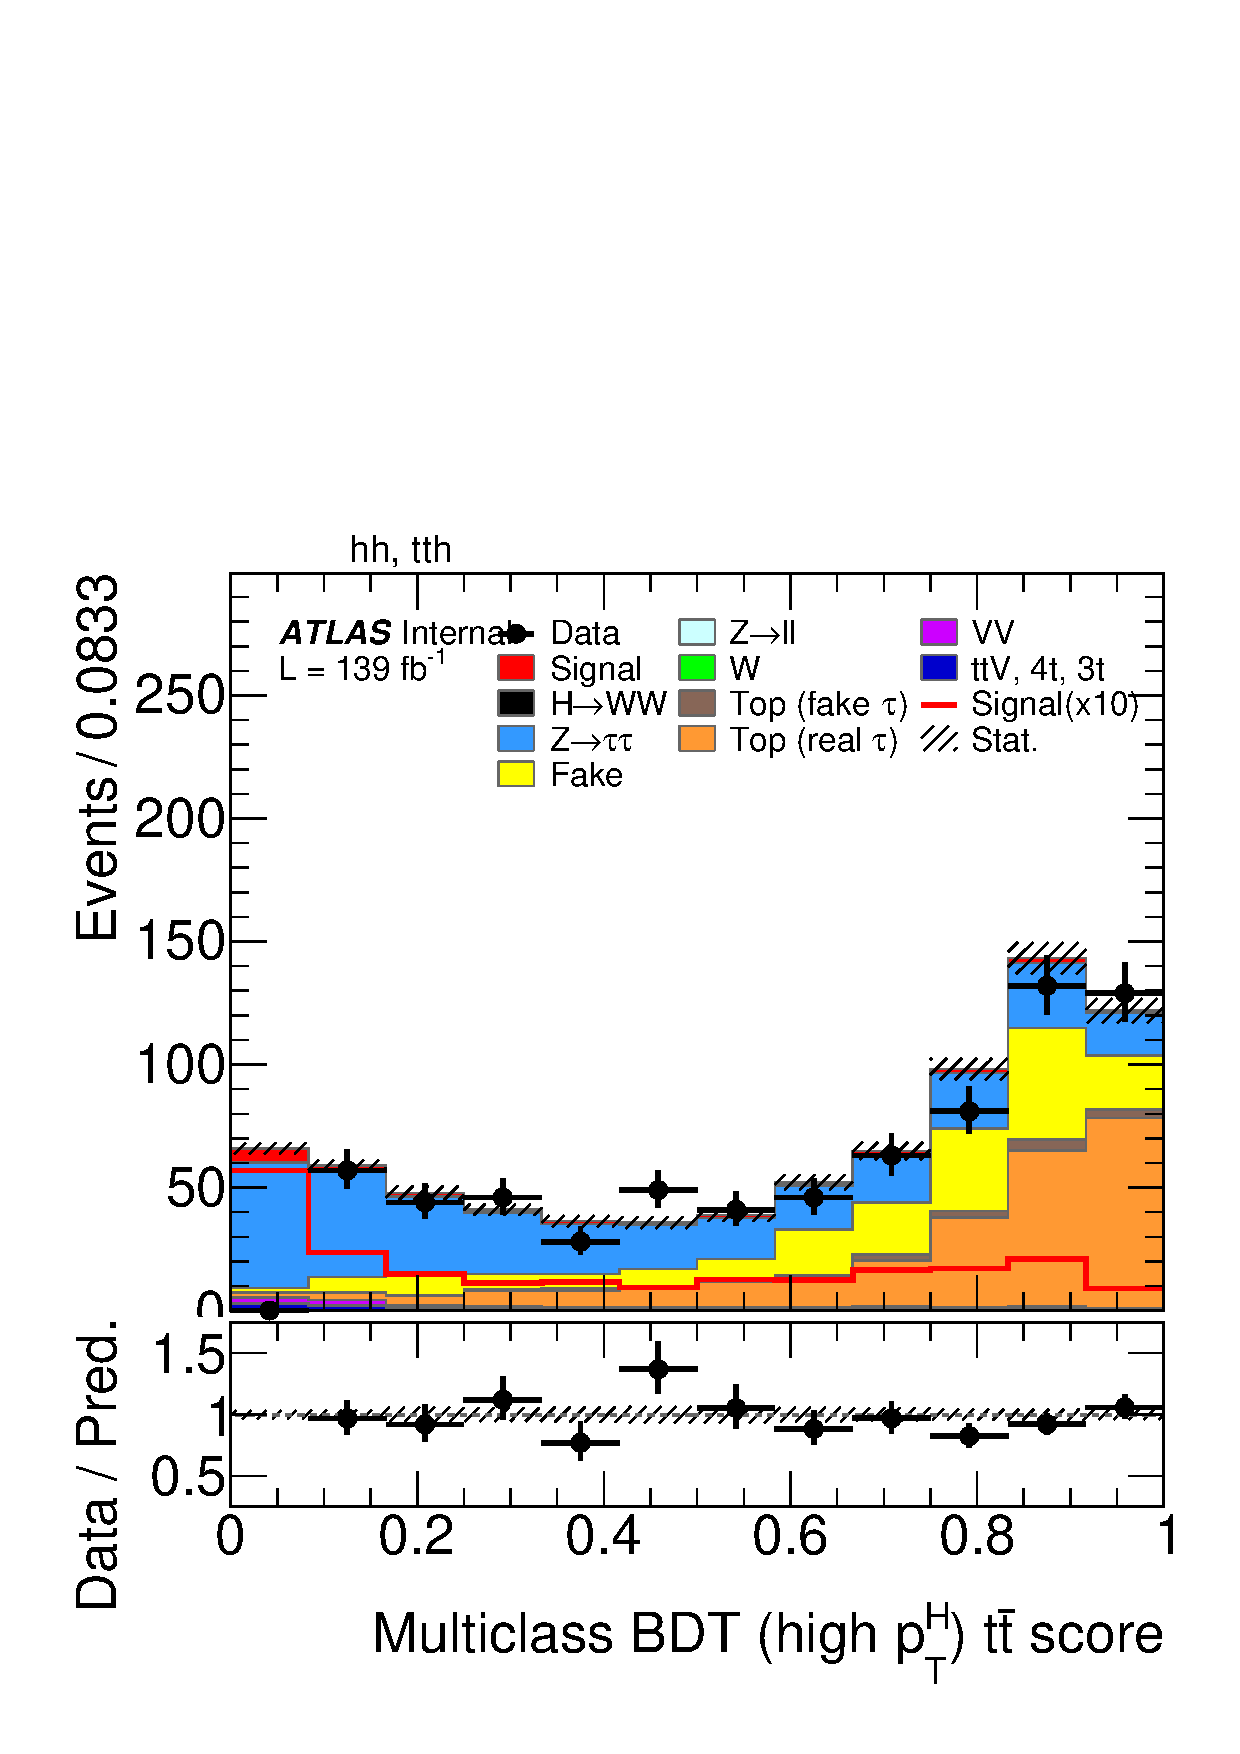
\includegraphics[width=0.32\textwidth]{images/plots_overtrain_gt200/plot_tth_ttbar_multiclass_gt200_hh_tth.pdf} 
  \end{tabular}
  \caption{Multiclass BDT score distributions for the high \pth training.}
  \label{highpt_modelling}
\end{figure}
%%%%%%%%%%%%%%%%%%%%%%%%%%%%%%%%%%%%%%%%%%%%%%%%%%%%%%%%%%%%%%%%%%%%%%%%%%%%%%%%%%%%%%%%%%%%%%%%%%%%%%%%%%%%%%%%%%%%%%%%%%%%%%%%%%%%%%%%%%%%%%%%%%%%%%%%%%%%%%%%%%%%%%%%%%%%%%%%%%%%
\section{Event categorization}
\label{sec:tth_categories}

In order to measure the signal strength of the process under study, while keeping the normalisation of the main backgrounds under control, SRs and CRs are defined, enriched in either signal or background events. These are obtained by applying requirements on the classifier scores provided by the multiclass BDT introduced above, from which a promising separation between the signal and the main background processes can be achieved, as illustrated in Figure~\ref{fig:triangle}.

\begin{figure}[htbp]
  \centering
  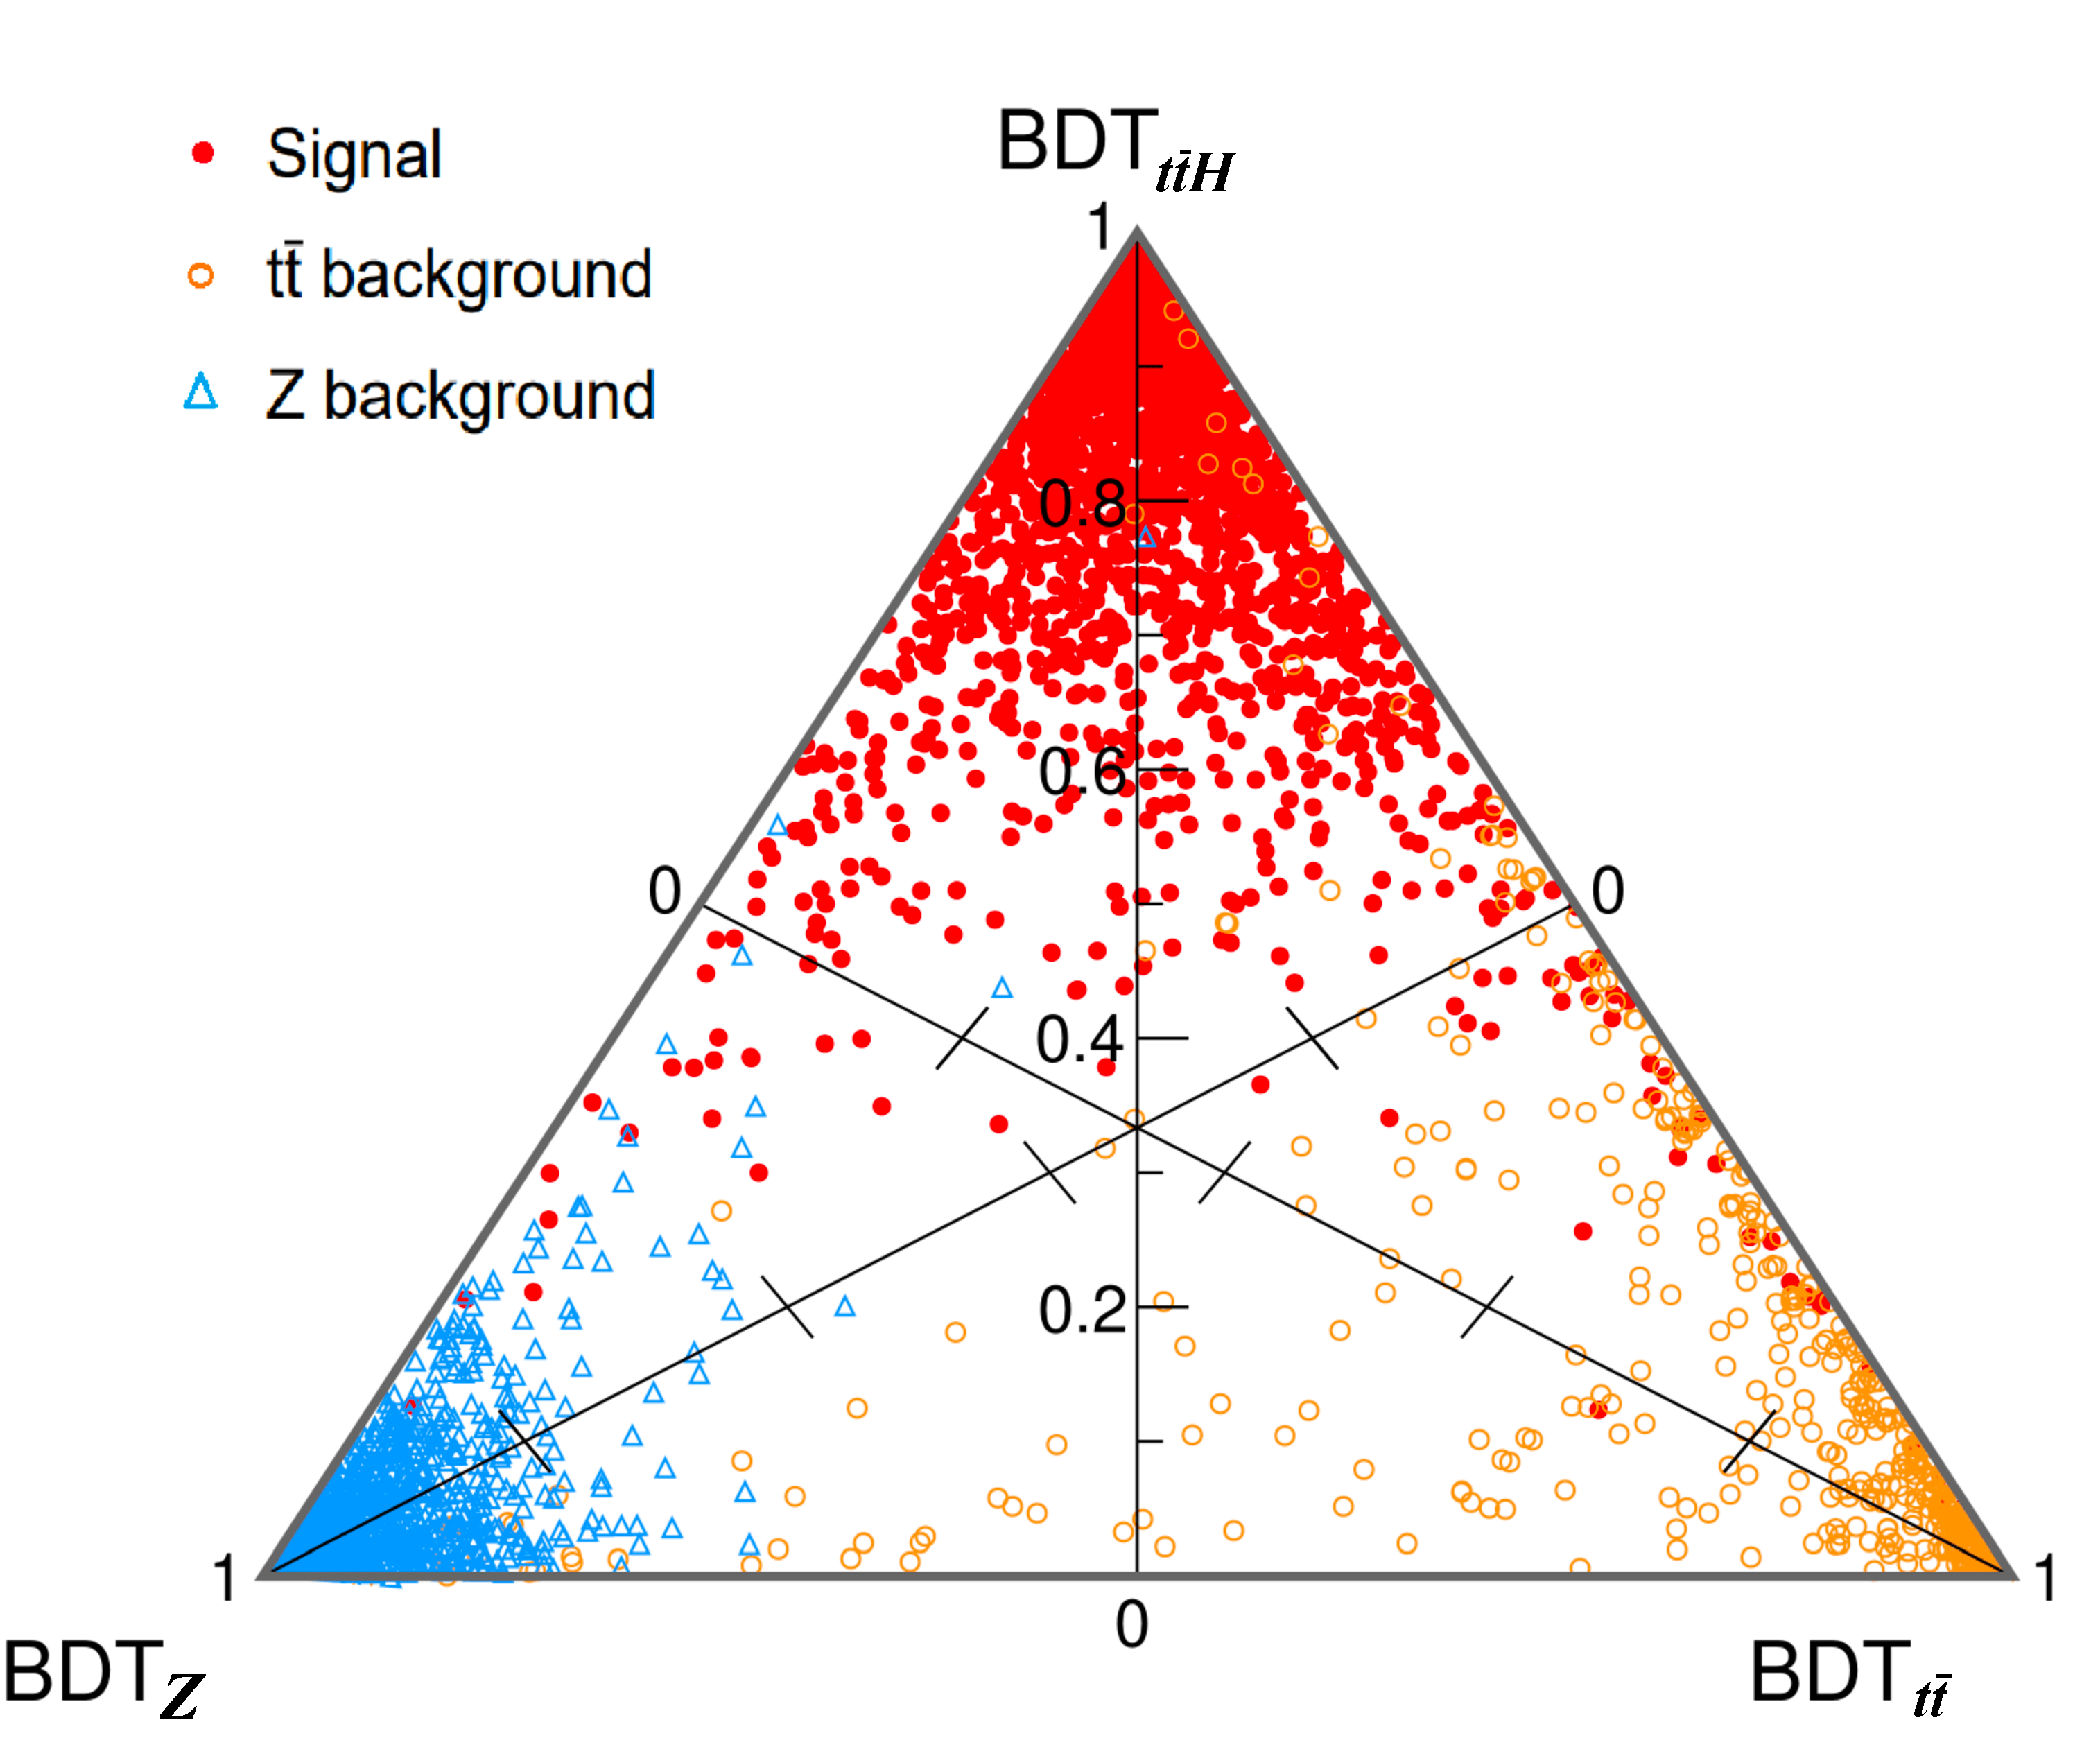
\includegraphics[width=0.6\textwidth]{triangle}
  \caption{Distributions of signal, \ztautau and \ttbar background MC events events in the plane defined by the three BDT scores in the Multiclass training, performed inclusively in \pth for this representation.}
  \label{fig:triangle}
\end{figure}

The requirements consist of rectangular cuts on each score, optimised to maximise the sensitivity to the corresponding process. The optimisation is performed through a one-dimensional scan of each class score, aiming to maximise the expected statistical significance of a counting experiment. As defined in Ref.~\cite{ATL-PHYS-PUB-2020-025}, this significance function computes the $Z$-value (the significance in standard deviations for a counting experiment) by testing a background-only hypothesis against a signal+background alternative. It accounts for the relative background uncertainty, treated as Gaussian-distributed, thereby providing a refined estimate compared to the simple $S/\sqrt{S+B}$ approximation. In this analysis, both the MC statistical uncertainties and an additional $10\%$ relative uncertainty, representative of \ttbar-related systematic effects (the most relevant in this channel) discussed in the next section, are considered.

The \ttH\ signal region is defined by performing the scan on the $\text{BDT}_{\text{\ttH}}$ score. The \ztautau control region is obtained from events lying outside the \ttH SR, by inverting the cut on the $\text{BDT}_{\text{\ttH}}$ score and subsequently applying the scan on the $\text{BDT}_{Z}$ score. Finally, the \ttbar control region is determined by inverting the cuts on the other two BDT scores, resulting in three orthogonal regions, taking advantage of the the normalisation of the multiclass scores mentioned before.

This procedure is applied to events in both regions (\pth $\gtrless 200$~\GeV) using the set of multiclass scores from the corresponding training, as shown in Table~\ref{tab:tth_cat}. Events in the SRs are further subdivided into three categories according to \pth ($<200$~GeV, $200-300$~GeV and $>300$~GeV) motivated by the \ttH STXS binning.

\begin{table}[h]
  \caption{Definition of the signal and control regions for the different \ttHtt categories as a function of the \pth. $\text{BDT}^{\text{low}}_{\text{\tth}}$ and $\text{BDT}^{\text{low}}_{Z}$ denote the \ttH and \ztautau scores from the low \pth training, while $\text{BDT}^{\text{high}}_{\text{\tth}}$ and $\text{BDT}^{\text{high}}_{Z}$ refer to the \tth and \ztautau scores from the high \pth training.}
  \centering
  \small
  \renewcommand{\arraystretch}{1.2}
  \setlength{\tabcolsep}{8.5pt}
  \begin{tabular}{l c|c c}
  \toprule
   & \multicolumn{3}{c}{\pth bins in GeV} \\
  \cmidrule(lr){2-4}
   & $<200$ & [200, 300] & $>300$ \\
  \midrule
  Signal region &
  $ \text{BDT}^{\text{low}}_{t\bar{t}H} > 0.65 $ &
  $ \text{BDT}^{\text{high}}_{t\bar{t}H} > 0.65 $ &
  $ \text{BDT}^{\text{high}}_{t\bar{t}H} > 0.65 $ \\
  \midrule
  $Z(\to \tau\tau)$ control region &
  \begin{tabular}[c]{@{}c@{}} 
  $ \text{BDT}^{\text{low}}_{t\bar{t}H} < 0.65 $ \\
  $ \text{BDT}^{\text{low}}_{Z} > 0.2 $ 
  \end{tabular} &
  \begin{tabular}[c]{@{}c@{}} 
  $ \text{BDT}^{\text{high}}_{t\bar{t}H} < 0.65 $ \\
  $ \text{BDT}^{\text{high}}_{Z} > 0.2 $ 
  \end{tabular} &
  \begin{tabular}[c]{@{}c@{}} 
  $ \text{BDT}^{\text{high}}_{t\bar{t}H} < 0.65 $ \\
  $ \text{BDT}^{\text{high}}_{Z} > 0.2 $ 
  \end{tabular} \\
  \midrule
  $t\bar{t}$ control region &
  \begin{tabular}[c]{@{}c@{}} 
  $ \text{BDT}^{\text{low}}_{t\bar{t}H} < 0.65 $ \\
  $ \text{BDT}^{\text{low}}_{Z} < 0.2 $ 
  \end{tabular} &
  \begin{tabular}[c]{@{}c@{}} 
  $ \text{BDT}^{\text{high}}_{t\bar{t}H} < 0.65 $ \\
  $ \text{BDT}^{\text{high}}_{Z} < 0.2 $ 
  \end{tabular} &
  \begin{tabular}[c]{@{}c@{}} 
  $ \text{BDT}^{\text{high}}_{t\bar{t}H} < 0.65 $ \\
  $ \text{BDT}^{\text{high}}_{Z} < 0.2 $ 
  \end{tabular} \\
  \bottomrule
  \end{tabular}
  \label{tab:tth_cat}
\end{table}

  
Moreover, the events classified in the signal regions for each \pth bin are further divided into two categories, already introduced in Section~\ref{sec:event_selection_background}: $\text{m}_{\tau \tau}$ sideband region and $\text{m}_{\tau \tau}$ window region in the Higgs boson mass. The window region contains events with a reconstructed Higgs boson mass within the interval $100 < m_{\tau\tau} < 150$~GeV, while the sideband region contains the remaining events. The window regions provide enhanced purity in signal events, whereas the sideband regions, despite their lower signal purity, can still be exploited to constrain the background processes in the signal regions of this analysis.

Figures~\ref{fig:bdt_ztt} and~\ref{fig:bdt_ttbar} show the BDT score distributions in data and MC for the \ztautau and \ttbar control regions, respectively, showing good agreement with the background predictions in the corresponding regions of phase space that are used to validate the normalisation of these backgrounds. Figure~\ref{fig:bdt_signal} presents the distributions of the \ttH BDT scores and the invariant mass in data for the defined SRs. Most of the bins are blinded so that, prior to performing the statistical fit, no data are shown in bins where a signal contribution above $5\%$ is expected, unless explicitly stated otherwise, in order to avoid any potential bias.

\begin{figure}[h]
  \centering
  \begin{subfigure}[b]{0.32\textwidth}
    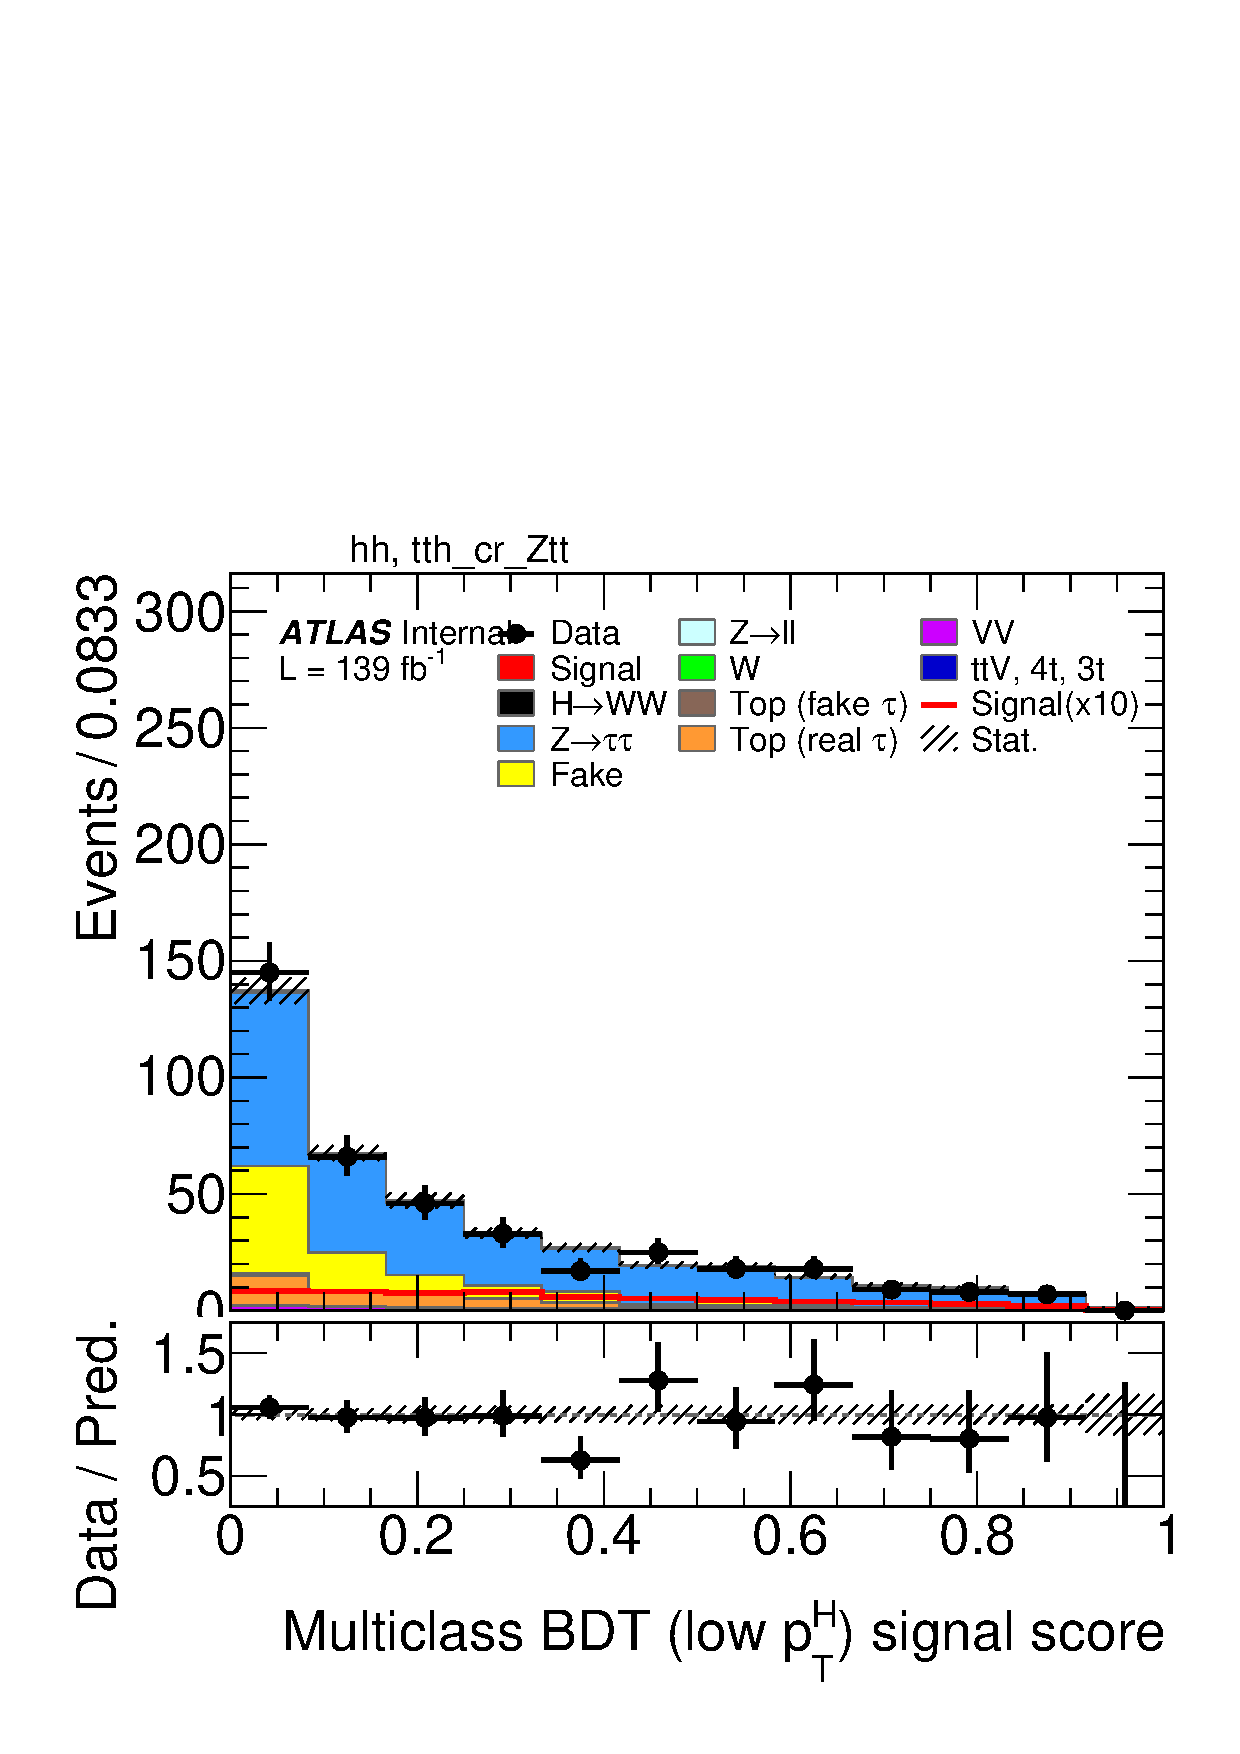
\includegraphics[width=\textwidth]{images/sr_cr_plots/plot_tth_signal_multiclass_lt200_hh_tth_cr_Ztt.pdf}
    \caption{}
  \end{subfigure}
  \begin{subfigure}[b]{0.32\textwidth}
    \includegraphics[width=\textwidth]{images/sr_cr_plots/plot_tth_ttbar_multiclass_lt200_hh_tth_cr_Ztt.pdf}
    \caption{}
  \end{subfigure}
  \begin{subfigure}[b]{0.32\textwidth}
    \includegraphics[width=\textwidth]{images/sr_cr_plots/plot_tth_Z_multiclass_lt200_hh_tth_cr_Ztt.pdf}
    \caption{}
  \end{subfigure}

  \begin{subfigure}[b]{0.32\textwidth}
    \includegraphics[width=\textwidth]{images/sr_cr_plots/plot_tth_signal_multiclass_gt200_hh_tth_cr_Ztt.pdf}
    \caption{}
  \end{subfigure}
  \begin{subfigure}[b]{0.32\textwidth}
    \includegraphics[width=\textwidth]{images/sr_cr_plots/plot_tth_ttbar_multiclass_gt200_hh_tth_cr_Ztt.pdf}
    \caption{}
  \end{subfigure}
  \begin{subfigure}[b]{0.32\textwidth}
    \includegraphics[width=\textwidth]{images/sr_cr_plots/plot_tth_Z_multiclass_gt200_hh_tth_cr_Ztt.pdf}
    \caption{}
  \end{subfigure}

  \caption{Distribution of the \ttH\ multiclass BDT scores in the $Z(\to\tau\tau)$ CR.  
  (a)–(c) correspond to the low-$p_{\mathrm{T}}^H$ training and (d)–(f) to the high-$p_{\mathrm{T}}^H$ training,  
  for the signal, \ttbar, and \ztautau\ classes, respectively. Only statistical uncertainties are shown.  
  Data are blinded for bins with a signal-over-background ratio above 5\%.}
  \label{fig:bdt_ztt}
\end{figure}


\begin{figure}[h]
  \centering
  \begin{subfigure}[b]{0.32\textwidth}
    \includegraphics[width=\textwidth]{images/sr_cr_plots/plot_tth_signal_multiclass_lt200_hh_tth_cr_ttbar.pdf}
    \caption{}
  \end{subfigure}
  \begin{subfigure}[b]{0.32\textwidth}
    \includegraphics[width=\textwidth]{images/sr_cr_plots/plot_tth_ttbar_multiclass_lt200_hh_tth_cr_ttbar.pdf}
    \caption{}
  \end{subfigure}
  \begin{subfigure}[b]{0.32\textwidth}
    \includegraphics[width=\textwidth]{images/sr_cr_plots/plot_tth_Z_multiclass_lt200_hh_tth_cr_ttbar.pdf}
    \caption{}
  \end{subfigure}

  \begin{subfigure}[b]{0.32\textwidth}
    \includegraphics[width=\textwidth]{images/sr_cr_plots/plot_tth_signal_multiclass_gt200_hh_tth_cr_ttbar.pdf}
    \caption{}
  \end{subfigure}
  \begin{subfigure}[b]{0.32\textwidth}
    \includegraphics[width=\textwidth]{images/sr_cr_plots/plot_tth_ttbar_multiclass_gt200_hh_tth_cr_ttbar.pdf}
    \caption{}
  \end{subfigure}
  \begin{subfigure}[b]{0.32\textwidth}
    \includegraphics[width=\textwidth]{images/sr_cr_plots/plot_tth_Z_multiclass_gt200_hh_tth_cr_ttbar.pdf}
    \caption{}
  \end{subfigure}

  \caption{Distribution of the \ttH\ multiclass BDT scores in the \ttbar CR.  
  (a)–(c) correspond to the low-$p_{\mathrm{T}}^H$ training and (d)–(f) to the high-$p_{\mathrm{T}}^H$ training,  
  for the signal, \ttbar, and \ztautau\ classes, respectively. Only statistical uncertainties are shown.  
  Data are blinded for bins with a signal-over-background ratio above 5\%.}
  \label{fig:bdt_ttbar}
\end{figure}


\begin{figure}[h]
  \centering
  \begin{subfigure}[b]{0.32\textwidth}
    \includegraphics[width=\textwidth]{images/sr_cr_plots/plot_tth_signal_multiclass_lt200_hh_tth_sr_pth_lt200.pdf}
    \caption{}
  \end{subfigure}
  \begin{subfigure}[b]{0.32\textwidth}
    \includegraphics[width=\textwidth]{images/sr_cr_plots/plot_tth_signal_multiclass_gt200_hh_tth_sr_pth_200_300.pdf}
    \caption{}
  \end{subfigure}
  \begin{subfigure}[b]{0.32\textwidth}
    \includegraphics[width=\textwidth]{images/sr_cr_plots/plot_tth_signal_multiclass_gt200_hh_tth_sr_pth_gt300.pdf}
    \caption{}
  \end{subfigure}

  \begin{subfigure}[b]{0.32\textwidth}
    \includegraphics[width=\textwidth]{images/sr_cr_plots/plot_ditau_mmc_mlm_m_hh_tth_sr_pth_lt200.pdf}
    \caption{}
  \end{subfigure}
  \begin{subfigure}[b]{0.32\textwidth}
    \includegraphics[width=\textwidth]{images/sr_cr_plots/plot_ditau_mmc_mlm_m_hh_tth_sr_pth_200_300.pdf}
    \caption{}
  \end{subfigure}
  \begin{subfigure}[b]{0.32\textwidth}
    \includegraphics[width=\textwidth]{images/sr_cr_plots/plot_ditau_mmc_mlm_m_hh_tth_sr_pth_gt300.pdf}
    \caption{}
  \end{subfigure}

  \caption{Distribution of the \ttH\ multiclass signal BDT scores (a–c) and \mmc distributions 
  (d–f) in the SRs at different \pth bins. Only statistical uncertainties are shown. Data are blinded for 
  bins with a signal-over-background ratio above 5\%.
  }
  \label{fig:bdt_signal}
\end{figure}


A summary of the expected purity of \ttHtt signal events in each signal region is shown in Figure~\ref{fig:tth_purity}. The diagonal structure of this submatrix indicates that the defined signal regions are highly pure in the \ttH process, with only some contamination mainly arising from ggF events at high \pth.

\begin{figure}[htbp]
  \centering
  \includegraphics[width=0.7\textwidth]{tth_purity}
  \caption{Expected SM \ttHtt signal purity in each SR of the analysis, shown as ``Reconstructed Category''. Adapted from Ref.~\cite{differential_htautau}.}
  \label{fig:tth_purity}
\end{figure}

%%%%%%%%%%%%%%%%%%%%%%%%%%%%%%%%%%%%%%%%%%%%%%%%%%%%%%%%%%%%%%%%%%%%%%%%%%%%%%%%%%%%%%%%%%%%%%%%%%%%%%%%%%%%%%%%%%%%%%%%%%%%%%%%%%%%%%%%%%%%%%%%%%%%%%%%%%%%%%%%%%%%%%%%%%%%%%%%%%%%
\section{Systematic Uncertainties}
\label{sec:tth_systematics}

Systematic uncertainties from multiple sources affect the measurement of the \ttH cross-section in the \tauhadhad channel, both in the signal and in the background estimation. They can be grouped according to their origin into experimental uncertainties, arising from detector performance and object reconstruction; theoretical uncertainties related to the modelling of the dominant backgrounds (\ttbar and \ztautau); and theoretical uncertainties affecting the prediction of the \ttH signal itself. Each type of uncertainty requires a dedicated treatment to propagate its impact into the analysis. 
In practice, systematic variations are typically evaluated through $\pm 1\sigma$ shifts, which are then propagated to the final distributions employed in the statistical fit.  

These uncertainties can also be distinguished by the way they impact our measurement. A first category is devoted to those affecting event weights, which modify how events are weighted within a given category. To account for these effects, alternative weight sets are applied on an event-by-event basis, and the resulting distributions are compared with the nominal case. Such variations can alter not only the overall normalization but also the shape and relative contribution of different processes. Since the event weights often depend on specific kinematic variables, these uncertainties propagate to both the normalization and the shape of the final distributions.  

A second category refers to uncertainties that impact the reconstructed kinematic properties of the events, such as the four-momenta of final-state objects. In this case, a full reprocessing of the event is required, recalculating derived quantities such as the \etmiss or the \mmc. Variations of this type can induce migrations of events between different analysis regions, altering the signal acceptance or modifying the kinematic distributions within a given category.  

The incorporation of systematic uncertainties in the likelihood statistical fit is discussed in Section~\ref{sec:statistical_tth}. The following subsections summarise the main sources of systematic uncertainties relevant for \ttHtt final state.

\subsection{Signal theoretical uncertainties}
\label{subsec:signal_theo_syst}

Theoretical uncertainties on the \ttH signal prediction are evaluated following the recommendations of the LHC Higgs Cross-Section Working Group~\cite{https://doi.org/10.23731/cyrm-2017-002, https://doi.org/10.5170/cern-2013-004}. These prescriptions ensure consistency across Higgs boson analyses and provide a common framework that allows results to be combined. The considered sources include parton distribution functions (PDFs), the strong coupling constant $\alpha_{s}$, QCD scale variations, as well as uncertainties related to parton shower modelling and to the choice of matrix-element generator.  

The impact of PDF uncertainties is estimated using the eigenvector variations of the \textsc{pdf4lhc\_nlo\_30} set, applied through the reweighting scheme implemented in the \textsc{powhegbox} generator. The resulting variations are treated as independent sources of uncertainty in the statistical model. The uncertainty in $\alpha_{s}$ is derived by varying its value around the central choice. 

For this production mode, QCD scale uncertainties are separated into six independent components. These include one uncertainty on the inclusive cross-section and five additional components corresponding to migrations between different \pth bins, following the STXS~1.2 definition (as shown in Figure~\ref{fig:STXSbins}).

Uncertainties associated with parton shower and matrix-element modelling are also included. They are assessed by comparing the nominal samples with alternative samples where the parton shower model is replaced by \textsc{Herwig7}, while keeping the same matrix-element generator, as explained in Section~\ref{subsec:higgs_mc}. This procedure allows for an evaluation of the systematic effects arising from the modelling of QCD radiation in \ttH signal events.

\subsection{Background theoretical uncertainties}
\label{subsec:bkg_theo_syst}

Theoretical uncertainties affecting the background prediction are particularly relevant for the dominant \ztautau and \ttbar processes.  

For the \ztautau background, several sources are considered, including uncertainties from the parton distribution functions, renormalization and factorization scales, the CKKW matching scheme, QCD scale factors, as well as uncertainties associated with the underlying event and the parton shower model. The PDF uncertainties are evaluated using 100 weight variations provided by the \textsc{sherpa} generator, based on the eigenvector variations of the \textsc{nnpdf3.0nnlo} set. The resulting variations are combined to obtain the total PDF uncertainty. 
Correlations between normalization and shape components of the PDF uncertainties are preserved between the \ztautau control region and the corresponding signal regions. This treatment ensures that normalization factors extracted in specific control regions do not artificially constrain the background description in other regions. Uncertainties from missing higher-order corrections are estimated by varying the factorization and renormalization scales, with the envelope of these variations taken as the systematic uncertainty.

An additional uncertainty is applied to cover modelling deficiencies in the electroweak component of the \ztautau\ background in the MC simulation. This component is estimated using MC samples, and a scale factor is derived by comparing the nominal \textsc{sherpa} prediction with alternative samples generated with different matrix-element generators. An uncertainty is then assigned to this scale factor, defined as the full difference between the unscaled prediction and the scaled template, with the upward variation obtained by symmetrization.  

For the top-quark related backgrounds, including inclusive \ttbar, the main sources of uncertainty are variations in the PDFs (evaluated using the 30 most relevant eigenvector variations of the chosen set), comparisons between different matrix-element generators while keeping the parton shower fixed, comparisons between parton shower models with a fixed matrix-element generator, and variations in initial- and final-state radiation. The latter are implemented through reweighting of the nominal predictions. These uncertainties are particularly relevant in this analysis where top-quark related backgrounds constitute a large fraction of the total background.

\subsection{Experimental uncertainties}
\label{subsec:exp_syst}

The most relevant experimental uncertainties arising from different detector components and reconstruction techniques for the \ttHtt final states are those associated with jets, hadronic $\tau$-leptons, \etmiss, $b$-tagging, and the integrated luminosity.  

Jet-related uncertainties are a major source of systematics. The jet energy scale (JES) uncertainty originates from multiple sources, including in-situ calibration, pile-up effects, high-$p_{\text{T}}$ extrapolations, and flavour-dependent responses of quark- and gluon-initiated jets~\ref{ATLAS_JES}. JES uncertainties are decomposed into several uncorrelated nuisance parameters describing flavour composition, flavour response, $b$-jet response, pile-up effects, and $\eta$-intercalibration. Additional nuisance parameters account for non-closure effects in specific $p_{\text{T}}$ and $\eta$ regions, as well as uncertainties related to tile calorimeter calibration. Jet energy resolution uncertainties are also included, impacting \etmiss and thereby the reconstructed di-$\tau$ mass (\mmc).  

Uncertainties related to \tauhad reconstruction include identification efficiency, energy scale, trigger efficiency, and the performance of the BDT used to reject electrons misidentified as $\tau$-leptons. The identification efficiency uncertainties, typically in the range 2-6\%, are derived from comparisons between data and MC and are decorrelated according to $p_{\text{T}}$. The energy scale uncertainty ranges between 1\% and 4\%, depending on momentum and track multiplicity, and is described by dedicated nuisance parameters. The trigger efficiency uncertainty is smaller (about 1-1.5\%).  

For $b$-tagging, uncertainties in the tagging efficiencies of $b$-jets, as well as mis-tag rates for $c$-jets and light-flavour jets, are considered~\ref{ATLAS_bjet_syst}. These are implemented through variations of scale factors derived from eigenvector decompositions of the associated covariance matrices. Additional parameters cover extrapolations to high-$p_{\text{T}}$ jets and the extension of $c$-jet calibrations to hadronic $\tau$-lepton jets.  

The uncertainties in the reconstruction of \etmiss mainly arise from the modelling of the soft term~\ref{ATLAS-CONF-2018-023}. Variations in its energy scale and resolution, both parallel and perpendicular to the hard-object $p_{\text{T}}$, are included as independent systematic sources.  

The uncertainty in the integrated luminosity affects the normalisation of signal and MC-based backgrounds. The absolute luminosity calibration carries an uncertainty of $\pm 0.83\%$, dominated by the extrapolation from low-$\mu$ calibration conditions to the data-taking periods~\ref{ATLAS-CONF-2019-021}. This uncertainty is applied coherently to all MC processes except those whose normalisation is directly constrained in data control regions.  

Finally, background estimation methods introduce further experimental uncertainties. In particular, in the \ttHtt channel, these uncertainties mainly arise from the statistical precision of the fake factors, whose derivation has been described in Section~\ref{sec:event_selection_background}.




%%%%%%%%%%%%%%%%%%%%%%%%%%%%%%%%%%%%%%%%%%%%%%%%%%%%%%%%%%%%%%%%%%%%%%%%%%%%%%%%%%%%%%%%%%%%%%%%%%%%%%%%%%%%%%%%%%%%%%%%%%%%%%%%%%%%%%%%%%%%%%%%%%%%%%%%%%%%%%%%%%%%%%%%%%%%%%%%%%%%
\section{Statistical fit}
\label{sec:statistical_tth}

In high-energy physics, statistical techniques provide the fundamental tools to interpret, quantify and extract meaningful information out of the experimental results obtained from collision data recorded by ATLAS.
In particular, the extraction of the Higgs boson signal strength and the measurement of production cross-sections rely on a solid statistical modelling of the data, which allows us to translate observed event yields into physics results. 
The statistical framework used for building and implementing the models in this analysis is \textsc{TRExFitter}~\cite{trexfitter}, which relies on the \textsc{HistFactory}~\cite{histfactory} format and the \textsc{RooFit}~\cite{roofit} and \textsc{RooStats}~\cite{roostats} environments for model definition and statistical interpretation. 

The analysis presented here focuses on the extraction of the signal strength for \ttHtt process in the fully hadronic decay channel, but this measurement is embedded within the global \htautau analysis performed by ATLAS. It combines the contributions from the other three main Higgs production modes (ggF, VBF, and $VH$) and the complementary $\tau_{\ell}\tau_{\mathrm{had}}$ and $\tau_{e}\tau_{\mu}$ final states. 
The global fit provides a consistent and simultaneous determination of the Higgs boson couplings to $\tau$-leptons, within which the $t\bar{t}H$ contribution is measured. 
In the following, the strategy adopted for the statistical modelling is described, focusing first on the construction of the binned likelihood model and then on the specific setup for the STXS measurement targeting the $t\bar{t}H$ signal.

\subsection{Binned likelihood model}
\label{likelihood_fit}

The global \htautau analysis is designed to measure several parameters of interest (POI) related to Higgs boson production. 
Within the so-called STXS measurement, the goal is to determine the inclusive cross-section $\sigma(pp \to H \to \tau\tau)$ by combining all production modes and decay channels, 
to measure separately the cross-sections for the four main production mechanisms ($\sigma^{\mathrm{ggF}}_{H\to\tau\tau}$, $\sigma^{\mathrm{VBF}}_{H\to\tau\tau}$, $\sigma^{VH}_{H\to\tau\tau}$, and $\sigma^{t\bar{t}H}_{H\to\tau\tau}$), 
and finally to extract the cross-sections in each of the STXS bins targeted in this analysis.

In all cases, a \textit{binned maximum-likelihood} fit is employed, using the distribution of the $m_{\tau\tau}$.
In the end, this procedure essentially relies on comparing the number of data events observed in each bin of the input distributions for every region with signal and background expectations. The data are assumed to follow a Poisson distribution in the bins of the input distributions. Consequently, the likelihood function used in this fit can be expressed as the product of the probability density functions of each bin, including both signal and control regions:

\begin{equation}
  \begin{aligned}
  \mathcal{L}(\vec{n}|\mu, \vec{\theta}, \vec{\lambda}, \vec{\gamma}) 
    &= \prod_{r } \prod_{i } 
       \text{Pois}(n_{r,i}|\mu, \vec{\theta}, \vec{\lambda}, \vec{\gamma}) \,
       \mathcal{L}_{\gamma}(\gamma_{r,i}) \\[0.4em]
    &\quad \times \prod_{p} \text{Gauss}(\theta^{0}_{p}|\theta_{p}, \sigma^{0}_{p}) \, .
  \end{aligned}
  \end{equation}
  Here, $r$ runs over all analysis regions and the index $i$ over all bins in each distribution. 
  The vector $\vec{n}$ denotes the observed data events in each bin, while $n_{r,i}$ refers to the specific number of events in bin $i$ of region $r$. 
  The signal yields are scaled by the signal strength modifiers, which are the parameters of interest of the fit, collected in the vector $\vec{\mu}$. 
  
  As discussed previously, MC simulations may correctly describe the shape of the distributions but not always their overall normalization. 
  For this reason, the dominant \ztautau\ and \ttbar\ backgrounds are rescaled with normalization factors, treated as free-floating parameters in the fit in the same way as the signal strengths. 
  These are represented by the vector $\vec{\lambda}$. 
  
  The systematic uncertainties described in Section~\ref{sec:tth_systematics} are incorporated into the likelihood function through nuisance parameters (NPs), 
  which affect the predicted signal and background yields in the binned distributions. 
  Auxiliary measurements provide constraints on the size of these effects, and the nuisance parameters are included via Gaussian constraint terms that multiply the Poisson likelihood components. 
  The vector $\vec{\theta}$ denotes these NPs, constrained by Gaussian terms with mean values $\theta^{0}_{p}$_
  
  The probability of observing $n_{r,i}$ events in bin $i$ of region $r$, 
  given the expected number of events in that bin, is described by the Poisson probability 
  $\text{Pois}(n_{r,i}|\vec{\mu},\vec{\theta},\vec{\lambda},\vec{\gamma})$. 
  This expectation depends on the signal strength modifiers, the normalization factors, and the nuisance parameters. 
  The expected yield in bin $i$ of region $r$ is expressed as
  \begin{equation}
  \sum_{k} \mu_k \, s_{r,i,k}(\vec{\theta}) \;+\; \gamma_{r,i} \, b_{r,i}(\vec{\theta},\vec{\lambda}),
  \end{equation}
  where the sum runs over the different signal processes $k$, 
  and $b_{r,i}(\vec{\theta},\vec{\lambda})$ denotes the expected background contribution in that bin. 
  The parameter $\gamma_{r,i}$ is introduced to account for the statistical uncertainty in the size of the simulated background sample in each bin, 
  and is treated as correlated across the different background processes. 
The Poisson probability therefore takes the form:
\begin{equation}
  \begin{aligned}
  \text{Pois}(n_{r,i}|\vec{\mu},\vec{\theta},\vec{\lambda},\vec{\gamma}) 
  &= \frac{\Big(\sum_{k} \mu_k \, s_{r,i,k}(\vec{\theta}) + \gamma_{r,i} \, b_{r,i}(\vec{\theta},\vec{\lambda}) \Big)^{n_i}}{n_i!} \\
  &\quad \times 
  e^{\!\Big[-\Big(\sum_{k} \mu_k \, s_{r,i,k}(\vec{\theta}) + \gamma_{r,i} \, b_{r,i}(\vec{\theta},\vec{\lambda}) \Big)\Big]}.
  \end{aligned}
  \end{equation}
  

  The model is fitted to data by maximizing the likelihood function, 
  from which the free parameters are extracted. 
  These include the signal strength modifiers, which rescale the different Higgs boson production modes, 
  and the normalization factors applied to the background contributions. 
  The following section describes the likelihood model used for the STXS measurement, 
  which is employed to extract the parameters of interest in this analysis.
  
\subsection{STXS measurement strategy}
\label{stxs_setup}
%aqui hay que meter el diagramita explicando cuantas SRs y CRs tenemos en total y tal, así como VR.

In the likelihood function constructed for the STXS measurement, several signal and control regions are taken into account, 
covering the different phase space regions considered for \ttHtt\ and other production modes included in the global \htautau\ analysis. 
Although a detailed description of the regions defined for processes other than \ttH\ is not provided here, 
Figure~\ref{fig:stxs_all_regions} displays all categories used in the statistical fit of this analysis. 
In addition, to complement this global overview, Figure~\ref{fig:stxs_srs_pois} shows all signal regions employed as inputs for the four production modes, 
together with the corresponding STXS bins targeted by each of them.

\begin{figure}[htbp]
  \centering
  \includegraphics[width=0.8\textwidth]{stxs_all_regions.pdf}
  \caption{Schematic summary of the fit model used in the analysis. All regions which are used directly in the combined fit are indicated. They are grouped by topology (Boosted or ggF (red), VBF (orange), $VH$ (green) and \ttH (blue)). The \ttH signal and control regions are only defined for the \tauhadhad channel. The \ztautau control regions are defined in each channel. The top-quark control regions in Boosted, VBF and VH are not defined for the \tauhadhad channel. The arrows indicate the free floating normalization factors which are acting on various regions~\cite{differential_htautau}.}
  \label{fig:stxs_all_regions}
\end{figure}

\begin{figure}[htbp]
  \centering
  \includegraphics[width=0.99\textwidth]{stxs_srs_pois.png}
  \caption{Schematic representation of the fit model, with the definition of the 18 parameters of interest (POIs) within the STXS framework shown on the left, and the signal categorization used to enhance the sensitivity to these POIs shown on the right.}
  \label{fig:stxs_srs_pois}
\end{figure}

%For the fit, a total of 38 analysis regions are considered for ggF in the Boost category, 
%including both CRs and the 18 SRs, corresponding to the same setup used in the previous round of the analysis~\cite{couplings}. 
%The $VH$ process follows the same strategy, with 14 categories in total, 6 of which are SRs. 
%For VBF, as mentioned earlier, the categorization strategy was updated in this new iteration of the analysis in order to improve its sensitivity, 
%in line with the approach adopted for \ttH. 
%As a result, the fit now includes 98 VBF categories targeting new STXS bins, with 16 SRs defined per channel.

The categorization procedure for \ttH described in Section~\ref{sec:tth_categories} provides the statistical fit with a total of six SRs and two inclusive CRs in \pth\ for the measurement of the \tauhadhad\ channel. 

The CRs are used to improve the constraints on the background processes by exploiting multi-bin histograms in \mmc\ for the \ttHtt\ case, 
where inclusive CRs were found to provide better performance and precision in the statistical fit compared to splitting them as a function of \pth. 
In contrast, validation regions (VRs) are defined in the low- and high-\pt\ regimes for \ztautau\ and \ttbar. They are not included in the fit itself, but are used to verify the modelling of the BDT scores in background-dominated regions kinematically close to the SRs, thereby providing confidence in the robustness of the signal strength extraction.

Using these inputs, and through the tools introduced at the beginning of this section, several measurements are performed. 
The total cross-section of $pp \to H \to \tau\tau$ is measured, 
extracted from a single POI corresponding to the production cross-section times the Higgs boson branching ratio into $\tau\tau$ as predicted by the SM.
The cross-section of each individual Higgs boson production mode discussed above is also measured, 
using four POIs, one for each process.
Finally, a global fit is performed in which a total of 18 POIs are measured, 
corresponding to the cross-sections in the STXS stage~1.2 bins. 
Among them, three POIs are dedicated to the three \pth\ bins defined for \ttH. 
As mentioned earlier, the original STXS granularity is not preserved, but instead the bins are merged to achieve a balance between maximizing sensitivity 
and accounting for the limited size of the signal sample. 
The 18 POIs defined within the STXS framework are illustrated with different colours in the central panel of Figure~\ref{fig:stxs_srs_pois}.

Before presenting the results, some aspects of the likelihood fit should be highlighted, as they are crucial for ensuring robustness and stability while keeping the minimization time under control.

The model is inherently complex, due to the large number of signal and control regions together with the many normalization factors, nuisance parameters and parameters of interest. 
Moreover, the limited size of the available MC samples can induce significant statistical fluctuations in the systematic templates, sometimes exceeding the size of the systematic effect itself. 
If left untreated, this noise can destabilize the fit and artificially inflate the impact of certain uncertainties. 
To mitigate these issues, the analysis applies several techniques that simplify the likelihood model where possible and suppress spurious fluctuations, while preserving the meaningful shape variations relevant for the measurement. 

In practice, these simplifications consist of pruning processes and systematic uncertainties with negligible impact, 
as well as applying symmetrization and smoothing to reduce unphysical fluctuations in the templates. 
Such treatments are particularly relevant in regions with low statistics, as can be \ttH, 
where systematic effects are less dominant compared to the statistical uncertainty. 
This ensures that the fit remains stable and unbiased, preventing spurious noise from inflating the uncertainties, 
while preserving the sensitivity to the process of interest.
\clearpage
%%%%%%%%%%%%%%%%%%%%%%%%%%%%%%%%%%%%%%%%%%%%%%%%%%%%%%%%%%%%%%%%%%%%%%%%%%%%%%%%%%%%%%%%%%%%%%%%%%%%%%%%%%%%%%%%%%%%%%%%%%%%%%%%%%%%%%%%%%%%%%%%%%%%%%%%%%%%%%%%%%%%%%%%%%%%%%%%%%%%
\section{STXS results}
\label{sec:results_ttH}

%aquí hablamos fundamentalmente de ttH, pero también se muestran los resultados finales con el resto de modos de producción y canales y se cuenta que para mas detalles sobre el resto de modos de produccion, categorizacion y tal que se mire el differential paper y que 
%se detalla en dataset.tex como se produjeron los samples de estos main production modes del boson de Higgs.

\subsection{Post-fit distributions}
\label{post_fit}

Since a binned likelihood fit is performed, the choice of binning for the \mtt distributions plays an important role. It is therefore optimised to ensure stability of the fit and to minimise the dependence of the signal strength measurements on statistical fluctuations due to the finite size of the background samples. This optimisation is implemented through a rebinning procedure applied to all distributions, such that the relative statistical uncertainty of the background remains below 20\% in all bins.

The \mtt distributions for the different analysis regions are presented below, with the binning already optimised to keep the background statistical uncertainties under control. In all cases, the number of signal events in each bin has been scaled using the signal strength obtained from the fit with a single POI dedicated to extracting the combined production cross-section.

Figure~\ref{fig:postfit_cr_both} shows the \mtt distributions in both the \ztautau and \ttbar control regions. The shaded areas indicate bins that are blinded under the conditions mentioned above. In addition to the signal, the MC samples of these two backgrounds are also scaled with NFs dedicated to each of them. These NFs, as well as the NPs affecting the prediction of both background and signal, will be discussed in the following section. The modelling between data and prediction is found to be satisfactory, also in both the low- and high-\pth regions, as illustrated in the \mtt distributions in the validation regions shown in Figure~\ref{fig:postfit_vr_all}.
% =======================
% Post-fit CRs (2 subfigs)
% =======================
\begin{figure}[htbp]
  \centering

  \begin{subfigure}[b]{0.48\textwidth}
    \centering
    \includegraphics[width=\linewidth]{fit_stxs/chan_hh__cat_tth_ttbar__cr_postFit.pdf}
    \caption{\small \ttbar\ control region}
    \label{fig:postfit_cr_ttbar}
  \end{subfigure}\hfill
  \begin{subfigure}[b]{0.48\textwidth}
    \centering
    \includegraphics[width=\linewidth]{fit_stxs/chan_hh__cat_tth_ztt__cr_postFit.pdf}
    \caption{\small \ztautau\ control region}
    \label{fig:postfit_cr_ztt}
  \end{subfigure}

  \caption{Post-fit distributions of \mmc\ in the \ttbar\ (a) and \ztautau\ (b) CRs for the \ttH\ analysis.}
  \label{fig:postfit_cr_both}
\end{figure}

% =======================
% Post-fit VRs (4 subfigs)
% =======================
\begin{figure}[htbp]
  \centering

  % ttbar VRs
  \begin{subfigure}[b]{0.48\textwidth}
    \centering
    \includegraphics[width=\linewidth]{fit_stxs/chan_hh__cat_tth_pth_lt200__vr_ttbar_postFit.pdf}
    \caption{\small \ttbar\ VR, $p_{\text{T}}^{H}<200$~GeV}
    \label{fig:postfit_vr_ttbar_lt200}
  \end{subfigure}\hfill
  \begin{subfigure}[b]{0.48\textwidth}
    \centering
    \includegraphics[width=\linewidth]{fit_stxs/chan_hh__cat_tth_pth_gt200__vr_ttbar_postFit.pdf}
    \caption{\small \ttbar\ VR, $p_{\text{T}}^{H}>200$~GeV}
    \label{fig:postfit_vr_ttbar_gt200}
  \end{subfigure}

  \vspace{0.45cm}

  % Z->tautau VRs
  \begin{subfigure}[b]{0.48\textwidth}
    \centering
    \includegraphics[width=\linewidth]{fit_stxs/chan_hh__cat_tth_pth_lt200__vr_ztt_postFit.pdf}
    \caption{\small \ztautau\ VR, $p_{\text{T}}^{H}<200$~GeV}
    \label{fig:postfit_vr_ztt_lt200}
  \end{subfigure}\hfill
  \begin{subfigure}[b]{0.48\textwidth}
    \centering
    \includegraphics[width=\linewidth]{fit_stxs/chan_hh__cat_tth_pth_gt200__vr_ztt_postFit.pdf}
    \caption{\small \ztautau\ VR, $p_{\text{T}}^{H}>200$~GeV}
    \label{fig:postfit_vr_ztt_gt200}
  \end{subfigure}

  \caption{Post-fit distributions of \mmc\ in the VRs for \ttbar\ and \ztautau, shown in low- and high-$p_{\text{T}}^{H}$ regimes.}
  \label{fig:postfit_vr_all}
\end{figure}

For the signal regions, Figure~\ref{fig:summary_all} presents a summary of the post-fit yields of the different processes expected and observed in data for the \ttHtt signal categories included in the fit. One bin is shown for each of them, but this representation should not be misunderstood: due to the very limited statistics in these SRs, a single bin had to be employed in the input distributions for the fit, with the only exception being the SR at \pth$<200$~GeV in the mass window ($100<$\mmc$<150$~GeV), with two bins.

\begin{figure}[htbp]
  \centering
  \includegraphics[width=0.7\linewidth]{fit_stxs/summary_srs_tth.pdf}
  \caption{Post-fit yields in the \ttH categories of the \tauhadhad channel. The
  signal yields are scaled by the signal strength obtained from the 1-POI fit. The
  window categories contains events with \mtt in the range $[100, 150]$~GeV, while
  events outside of this mass region are included in the sideband region.}
  \label{fig:summary_all}
\end{figure}


%%%%%%%%%%%%%%%%%%%%%%%%%%%%%%%%%%%%%%%%%%%%%%%%%%%%%%%%%%%%%%%%%%%%%%%%%%%%%%%%%%%%%%%%%%%%%%%%%%%%%%%%%%%%%%%%%%%%%%%%%%%%%%%%%%%%%%%%%%%%%%%%%%%%%%%%%%%%%%%%
\subsection{Cross-section measurements}
\label{xsect}

The results obtained for the measurement of the signal strength extracted through the different POIs in the various fit parametrisations are presented below. 
For completeness, the 1-POI and 4-POI fits are firstly introduced. The 1-POI fit allows us to extract the inclusive cross-section of $pp \to H \to \tau \tau$. The best-fit value obtained for the signal strength, defined over the SM prediction, is 
$\mu(pp \to H \to \tau \tau) = 0.99^{+0.13}_{-0.11} = 0.99 \pm 0.07 (\text{stat.})^{+0.10}_{-0.09}(\text{syst.})$. 
This measurement of the signal strength improves by $25\%$ with respect to the previous analysis, which yielded $\mu_{\ttH} = 1.06^{+1.28}_{-1.08}$. The inclusive cross-section extracted from this measurement is:
\begin{equation}
  \sigma(pp \to H \to \tau\tau) 
  = 3.14 \pm 0.22 \, \text{(stat.)}^{+0.32}_{-0.29} \, \text{(syst.)} 
  = 3.14^{+0.41}_{-0.35} \, \text{pb}.
  \label{eq:htautau_xs}
  \end{equation}
  which is consistent with the SM prediction of $3.17 \pm 0.09$~pb~\cite{https://doi.org/10.23731/cyrm-2017-002}, within uncertainties, with a $p$-value for the compatibility test of 0.97, showing good agreement. 

  The \ttHtt cross-section can also be extracted from the 4-POI fit, where the signal strengths of the four main production modes are targeted in a simultaneous fit. For the case of \ttH, the observed cross-section extracted from the data is:
\begin{equation}
  \sigma(t\bar{t}H(\tau\tau))
  = 0.02^{+0.03}_{-0.02}(\text{stat.}) \pm 0.02(\text{syst.})~\text{pb} 
  = 0.02^{+0.03}_{-0.02}~\text{pb},
\end{equation}
which is also found to be in good agreement with the SM hypothesis of $0.031 \pm 0.003$~pb. The simultaneous 4-POI fit also yields satisfactory compatibility with the SM, with a measured $p$-value of 0.99. Figure~\ref{fig:permode_mu} summarises the signal strength measurements obtained for the four POIs in the simultaneous fit per production mode, as well as for the inclusive measurement of this parameter in the \htautau production process.

% =========================
% Plot 1: per-production-mode (1-POI y 4-POI)
% =========================
\begin{figure}[htbp]
  \centering
  \includegraphics[width=0.75\linewidth]{images/fit_stxs/4_poi_stxs.pdf} % <-- sustituye ruta/nombre
  \caption{Measured values of \(\sigma_H \times \mathcal{B}(H\!\to\!\tau\tau)\) relative to the SM expectation
  in the single-parameter (``Combined'') and per–production–mode (4–POI) fits.
  Error bars show the total uncertainty; the coloured band indicates the systematic component.}
  \label{fig:permode_mu}
\end{figure}

%=========%=========%=========%=========
%         STXS RESULTS
%=========%=========%=========%=========

Finally, focus is placed on the so-called 18-POI fit, which constitutes the main measurement of this analysis. In this fit, a parameter of interest is assigned to each STXS bin parametrising the different signals considered in this \htautau analysis, and the resulting signal strengths for the 18 STXS bins under study are shown in Figure~\ref{fig:stxs_mu}.
The measurement for the three POIs parametrising the \ttH signal in the three \pth bins considered is reported together with the corresponding cross-section:
\begin{itemize}
  \small
  \item $p_{\text{T}}^{H} < 200$~GeV:  
  \[
  \sigma \times B(H \to \tau\tau)=0.056^{+0.046}_{-0.044} 
  = 0.056^{+0.023}_{-0.019}(\text{syst.})\pm 0.035(\text{stat.})\text{pb}
  \]
  \[
  \mu \;=\; 2.2^{+1.8}_{-1.5}=2.2^{+0.84}_{-0.75}(\text{syst.})\pm 1.5(\text{stat.})
  \]
  \item $200 \leq p_{\text{T}}^{H} < 300$~GeV:  
  \[
  \sigma \times B(H \to \tau\tau) \;=\; -0.009^{+0.005}_{-0.005} 
  = -0.009^{+0.003}_{-0.004}(\text{syst.})\pm 0.003(\text{stat.}) \text{pb}
  \]
  \[
  \mu=-2.2^{+1.3}_{-1.1}=-2.2^{+0.58}_{-0.68}(\text{syst.})\pm 1.1(\text{stat.})
  \]
  \item $p_{\text{T}}^{H} \geq 300$~GeV:  
  \[
  \sigma \times B(H \to \tau\tau) \;=\; 0.029^{+0.023}_{-0.018} 
  = 0.029^{+0.009}_{-0.008}(\text{syst.})^{+0.021}_{-0.017}(\text{stat.})\text{pb}
  \]
  \[
  \mu=3.6^{+2.9}_{-2.3}=3.6^{+1.3}_{-0.9}(\text{syst.})^{+2.6}_{-2.1}(\text{stat.})
  \]
\end{itemize}

% =========================
% Plot 2: STXS (Stage 1.2) bin-by-bin
% =========================
\begin{figure}[htbp]
  \centering
  \includegraphics[width=0.92\linewidth]{images/fit_stxs/fig_06.pdf} % <-- sustituye ruta/nombre
  \caption{Results for \(\sigma_H \times \mathcal{B}(H\!\to\!\tau\tau)\) normalised to the SM prediction
  in the simplified template cross-section (STXS, stage~1.2) measurement.
  Each point corresponds to one STXS bin; error bars represent the total uncertainty and shaded bands the systematic component.}
  \label{fig:stxs_mu}
\end{figure}

% =========================
\subsubsection*{Normalization factors}
\label{nfs}
% =========================

Regarding the best-fit values obtained for the background normalization factors, encapsulated through free-floating parameters in the fit, the results for \ztautau\ and \ttbar\ in the \ttHtt\ channel are presented below. 
From the 18-POI fit, the best-fit value for the \ztautau\ normalization factor is found to be 
\(\text{NF}_{Z} = 1.20 \pm 0.16\), while for \ttbar\ the result is \(\text{NF}_{\ttbar} = 1.06 \pm 0.26\). 
%These values remain stable with respect to the signal parametrization or fit setup employed, as illustrated in Figure~\ref{fig:nfs_tth}, where the best-fit values of the \ttHtt\ normalization factors are shown for the three fit configurations considered. 

It is worth emphasizing that the top-quark normalization factor consistent with unity within one standard deviation, 
whereas the \ztautau\ normalization factor lies above the nominal value. 
This behaviour mainly reflects the need to correct mismodelling effects in the prediction of this background, largely driven by the sizeable contribution of jets originating from QCD processes.

%\begin{figure}[htbp]
%  \centering
%  \includegraphics[width=0.7\linewidth]{fit_stxs/nfs_tth.pdf}
%  \caption{Background normalization factors for \ttbar and \ztautau in \ttH
%  \tauhadhad channel for the different fit setups (1, 4 and 18-POI fits).}
%  \label{fig:nfs_tth}
%\end{figure}

% =========================
\subsubsection*{Nuisance parameters}
\label{nps}
% =========================

Concerning the nuisance parameters (NPs) associated with the various sources of systematic uncertainty affecting the analysis, those with the largest impact or relevance are presented below.
Although they are not the primary parameters of interest, they shape the fit outcome and in determining the overall uncertainty on the signal strength measurement. 

During the fit, the best-fit value of a nuisance parameter may deviate from its nominal expectation, in which case the parameter is said to be \emph{pulled}. 
If the data provide sensitivity to the associated systematic uncertainty, the fit may also reduce its pre-fit uncertainty, leading to a \emph{constraint}. 

Table~\ref{tab:combined_tth_uncert_summary} shows the grouped impact of systematic uncertainties affecting the measurements previously presented. The impact is grouped by source of systematic uncertainties, and it is shown for the 
combined fit (1-POI) and for the \ttH measurements in both the per-production-mode fit and in the 18-POI fit, showing the impact in the three \ttH POIs.

\begin{sidewaystable*}[htbp]
  \centering
  \footnotesize
  \renewcommand{\arraystretch}{1.2}
  \caption{Breakdown of the uncertainty contributions to the measured \(\sigma \times \mathcal{B}(H\!\to\!\tau\tau)\), relative to the SM expectation, for the combined (1-POI) fit, for \ttH\ in the 4-POI fit, and for the three \ttH\ STXS bins in the 18-POI fit. Experimental uncertainties for reconstructed objects include efficiency and energy/momentum scale and resolution effects. ``Samples size'' includes bin-by-bin statistical uncertainties in simulated backgrounds as well as those in the misidentified-\(\tau\) background estimated from data. Entries with negligible impact are denoted by “--”.}
  \label{tab:combined_tth_uncert_summary}
  \begin{tabular}{
      l
      c  % Combined
      c  % ttH (4POI)
      c
      c
      c
    }
    \toprule
    \textbf{Uncertainty source} & \textbf{Combined} & \textbf{\ttH} & \textbf{\ttH\ 0--200 GeV} & \textbf{\ttH\ 200--300 GeV} & \textbf{\ttH\ $>$300 GeV} \\
    \midrule
    Best-fit value                  & 0.99 & 0.77 & 2.1 & 2.2 & 3.6 \\
    Total uncertainty               & $\pm$0.12 & $\pm$0.97 & $\pm$1.7 & $\pm$1.2 & $\pm$2.6 \\
    \addlinespace[0.3em]
    Statistical uncertainty         & $\pm$0.07 & $\pm$0.82 & $\pm$1.5 & $\pm$0.9 & $\pm$2.4 \\
    Total systematic uncertainty    & $\pm$0.09 & $\pm$0.51 & $\pm$0.8 & $\pm$0.7 & $\pm$1.0 \\
    \midrule
    Background samples size                    & $\pm$0.03 & $\pm$0.31 & $\pm$0.5 & $\pm$0.5 & $\pm$0.5 \\
    Theoretical uncertainty in signal     & $\pm$0.08 & $\pm$0.12 & $\pm$0.3 & $\pm$0.2 & $\pm$0.5 \\
    Jet and \(E_{\mathrm{T}}^{\mathrm{miss}}\) & $\pm$0.03 & $\pm$0.15 & $\pm$0.5 & $\pm$0.2 & $\pm$0.2 \\
    Hadronic \(\tau\)-lepton decays        & $\pm$0.02 & $\pm$0.09 & $\pm$0.1 & $\pm$0.1 & $\pm$0.2 \\
    Misidentified background         & $\pm$0.02 & $\pm$0.05 & $\pm$0.1 & $\pm$0.1 & $\pm$0.1 \\
    Luminosity                       & -- & $\pm$0.01 & -- & -- & $\pm$0.1 \\
    Theoretical uncertainty in top-quark processes & -- & $\pm$0.31 & $\pm$0.4 & $\pm$0.4 & $\pm$0.6 \\
    Theoretical uncertainty in \(Z\!+\)jets & $\pm$0.01 & $\pm$0.08 & $\pm$0.1 & -- & $\pm$0.2 \\
    Flavour tagging                  & $\pm$0.01 & $\pm$0.05 & $\pm$0.1 & -- & $\pm$0.1 \\
    Electrons and muons              & $\pm$0.01 & $\pm$0.02 & -- & -- & -- \\
    \bottomrule
  \end{tabular}
\end{sidewaystable*}

As discussed, the measurement of the \ttH\ production cross-sections is largely dominated by statistical uncertainties from the data, 
which suggests that a significant improvement could be achieved with a larger dataset. 
Focusing on the impact of the grouped systematic uncertainties in the measurement of the \ttH\ signal strength across the three STXS bins in \pth considered in the 18-POI fit provides a more detailed view of how the different sources discussed previously affect each phase-space region. 
The dominant contribution generally arises from the statistical uncertainty associated with the limited size of the background samples. Uncertainties in the modelling of the top-quark backgrounds are of comparable importance, followed by those in the signal prediction. 
A slightly larger impact is also observed from the jet energy scale and resolution, as expected given that the analysis targets regions of the phase space with a high jet and $b$-jet multiplicity.

When examining the impact on the inclusive \ttH\ measurement from the 4-POI fit, a picture consistent with that discussed in the 18-POI fit is observed, with a comparatively larger impact from the systematic uncertainties related to the modelling of top-quark background.

In the case of the 1-POI fit, the measurement is instead dominated by systematic uncertainties, 
since all \htautau\ regions are included in the analysis, many of them with large statistics such as the ggF categories. 
Here, the leading systematic uncertainty is the theoretical uncertainty associated with the signal prediction.

Now concerning the constraints on NPs with the largest impact, 
Figures~\ref{fig:constraint_ttH} show the best-fit values of those NPs related to the modeling of parton showers and hadronization in the signal, 
as well as to the choice of matrix element generator and to the theoretical uncertainties in the prediction of top-quark background processes. 
The presented values are obtained from the STXS fit. 

Focusing first on the NPs associated with the theoretical signal uncertainties of \ttH, no significant pulls or constraints from the data are observed, 
and the best-fit values remain consistent with the pre-fit expectations within one standard deviation. 
On the other hand, for the NPs corresponding to top-quark background theoretical uncertainties,
stronger constraints are observed, particularly for the parameters linked to the choice of matrix element generator and to the modeling of parton showers. 
These systematics induce large normalization effects in the top-quark background, and are ultimately constrained thanks to the high statistics and purity of the \ttbar\ control region defined in the analysis, shown in Figure~\ref{fig:postfit_cr_ttbar}.

% ===========================================================
% Most important NPs Constraint plot for ttH
% ===========================================================
\begin{figure}[htbp]
  \centering
  \includegraphics[width=0.75\textwidth]{images/fit_stxs/STXS_combine_all_xs_NP_theory_top_signal.pdf}
  \caption{Nuisance parameters associated with theoretical uncertainties related to the signal and top-quark background modellings. The bestfit values of the nuisance parameters are shown for the 18-POI fit.}
  \label{fig:constraint_theory_sig}
\end{figure}

As already discussed in Table~\ref{tab:combined_tth_uncert_summary}, the grouped systematic uncertainties with the largest impact on the measurement of the three \ttH\ POIs can be identified. 
Figure~\ref{fig:ranking_tth_bins} provides a complementary representation of this information, showing both the impact and the pull of the nuisance parameters (NPs) associated with each source of uncertainty. 
For each NP $\theta$, the impact $\Delta\mu$ is defined as the change in the best-fit value of the POI when the NP is shifted by its uncertainty. 
Two cases are considered: the \textit{pre-fit} impact, obtained with a $\pm 1\sigma$ variation, and the \textit{post-fit} impact, where the variation can be reduced according to the constraints imposed by the fit. 
The ranking plots highlight the NPs with the largest effect on each POI, displaying both pre-fit and post-fit impacts together with the corresponding pulls.
% ===========================
% Ranking plots for ttH pT^H bins (stacked layout)
% ===========================
\begin{figure}[htbp]
  \centering

  % Row 1
  \begin{subfigure}[b]{0.45\textwidth}
    \centering
    \includegraphics[width=\linewidth]{images/fit_stxs/Ranking_r_9_ttH_ptH_0_200.png}
    \caption{\small $p_{\text{T}}^{H}<200$~GeV}
    \label{fig:ranking_tth_ptH_0_200}
  \end{subfigure}\hfill
  \begin{subfigure}[b]{0.45\textwidth}
    \centering
    \includegraphics[width=\linewidth]{images/fit_stxs/Ranking_r_10_ttH_ptH_200_300.png}
    \caption{\small $200<p_{\text{T}}^{H}<300$~GeV}
    \label{fig:ranking_tth_ptH_200_300}
  \end{subfigure}

  % Row 2
  \vspace{0.4cm}
  \begin{subfigure}[b]{0.45\textwidth}
    \centering
    \includegraphics[width=\linewidth]{images/fit_stxs/Ranking_r_11_ttH_ptH_gt300.png}
    \caption{\small $p_{\text{T}}^{H}>300$~GeV}
    \label{fig:ranking_tth_ptH_gt300}
  \end{subfigure}

  \caption{Ranking plots for the \ttH\ POIs in the three $p_{\text{T}}^{H}$ bins.
  The 20 nuisance parameters (NPs) with the largest impact on the signal strengths are shown. 
  Empty (filled) rectangles represent the pre-fit (post-fit) impact of the parameters. 
  Black points and error bars represent the post-fit values and uncertainties of the NPs, 
  while the markers of the background NFs show their pull with respect to the nominal value of 1.}
  \label{fig:ranking_tth_bins}
\end{figure}

As already anticipated, the dominant systematic uncertainties impacting the signal strength measurements are those associated with the theoretical modeling of the top-quark background. 
These include uncertainties from the parton shower, the matrix element calculation, and the description of ISR and FSR. 
In addition, the normalization factor of the top-quark background exhibits a sizeable uncertainty, particularly in the lowest $p_{\text{T}}^{H}$ bin (more populated by this type of background events). 
Uncertainties in the matrix element calculation for the \ttH\ signal itself are also non-negligible across the three $p_{\text{T}}^{H}$ bins. 
Further important contributions arise from the jet energy scale and resolution, as well as from the reconstruction and identification of $\tau$-leptons.
% =========================
\subsubsection*{Upper exclusion limits on \ttH}
\label{limits}
% =========================
From all these results it can be concluded that, as already mentioned, the extraction of signal from the three STXS bins is largely limited by the statistical uncertainties associated with the small dataset available. Nevertheless, no significant deviations from the SM are observed in any of the bins, with the largest deviation occurring in the intermediate-$p_{\text{T}}^{H}$ region ($200 < p_{\text{T}}^{H} < 300$~GeV), at the level of about 1.5$\sigma$. Consequently, the sensitivity to this signal in the 18-POI STXS fit remains rather limited.

To further quantify the constraints, 95\% confidence level (CL) upper exclusion limits are computed, using the $\text{CL}_{s}$ method~\cite{JUNK1999435,ALRead_2002}, for the $t\bar{t}H$ production mode, given the limited sensitivity of this process in the nominal 18-POI STXS fit due to the small statistics in this channel. The observed and expected limits are shown in Figure~\ref{fig:tth_cls_limits}, including the expected limits under both the background-only hypothesis ($\mu=0$) and when injecting SM signal ($\mu=1$). 

These exclusion limits provide an important cross-check of the measurement, as they quantify the maximum signal strength still compatible with the observed data in the absence of a significant excess. In practice, they ensure that even in regions where the sensitivity is insufficient to obtain a precise signal strength measurement, the analysis still constrains the parameter space by setting meaningful upper bounds on the production rate. Specifically, the observed limits correspond to factors of about 5.4, 2.2, and 9.2 times the SM prediction in the low-, intermediate-, and high-$p_{\text{T}}^{H}$ bins, respectively. 

%Habría que explicar lo que son los limites.
% =========================
% Plot 3: ttH pT^H-bin CLs limits
% =========================
\begin{figure}[htbp]
  \centering
  \includegraphics[width=0.70\linewidth]{images/fit_stxs/fig_08.pdf} % <-- sustituye ruta/nombre
  \caption{Upper limits at 95\% CL on the \ttH\ simplified template cross-sections in the individual $p_{\mathrm{T}}^{H}$ bins, shown relative to their SM expectation and derived using the $CL_s$ method. The observed limits are indicated by solid black lines, while the expected limits under the background-only (SM) hypothesis are shown with dotted black (red) lines. For the background-only case, the $\pm 1\sigma$ and $\pm 2\sigma$ uncertainty bands are also displayed.}
  \label{fig:tth_cls_limits}
\end{figure}








